\documentclass[journal]{IEEEtran}
\usepackage{amsmath,amsfonts}
\usepackage{algorithmic}
\usepackage{array}
\usepackage{textcomp}
\usepackage{stfloats}
\usepackage{booktabs}  
\usepackage{multirow} 
\usepackage{stackengine}
\usepackage{tabularx}
\renewcommand{\baselinestretch}{1.0} % IEEE line spacing standard
\usepackage{url}
\usepackage{verbatim}
\usepackage{graphicx}
\hyphenation{op-tical net-works semi-conduc-tor IEEE-Xplore}
\def\BibTeX{{\rm B\kern-.05em{\sc i\kern-.025em b}\kern-.08em
		T\kern-.1667em\lower.7ex\hbox{E}\kern-.125emX}}
\usepackage{balance}
\usepackage{makecell}
\usepackage{stfloats}  
\usepackage{comment}
\usepackage{geometry}
\usepackage{multirow}
\usepackage{tikz}
\usepackage{tikz-3dplot}
%\usetikzlibrary{positioning, shapes.geometric, decorations.pathreplacing, calc}
\usepackage{subcaption} 
\geometry{margin=1in}

\begin{document}
	\title{Wideband MVDR Beamforming and Dual-Channel Transformer Network for Acoustic Fault Diagnosis}
    % \title{Microphone Array MVDR Beamforming with Dual-Channel Transformer for Acoustic Fault Diagnosis}
    
    % \title{Joint Spatial Filtering and Deep Feature Learning for Acoustic Fault Diagnosis}
	\author{Zonglong Bai, Chen Yang}

	\maketitle
	\begin{abstract}
		This paper presents a novel approach for fault diagnosis using microphone array-based MVDR beamforming combined with deep learning. The method utilizes a microphone array to capture acoustic signals from faulty equipment. Room impulse responses (RIR) are employed to accurately model the acoustic propagation environment and achieve precise signal enhancement while suppressing interference. Wideband MVDR beamforming is implemented to perform joint spatial-frequency filtering. A dual-channel transformer network is introduced to further improve the classification performance. Experimental results demonstrate a significant improvement in Signal-to-Interference-plus-Noise Ratio (SINR) of 22.66 dB in strong interference environments, and the classification accuracy is also significantly improved. The proposed method shows great potential for real-world fault diagnosis applications in noisy industrial environments.
	\end{abstract}
	
	\begin{IEEEkeywords}
		Fault diagnosis, microphone array, beamforming, dual-channel Transformer network, acoustic signal processing
	\end{IEEEkeywords}

\section{Introduction}
Fault diagnosis is crucial for maintaining system reliability and preventing catastrophic failures. Traditional diagnostic methods rely primarily on vibration analysis and electrical parameter monitoring. However, acoustic signal analysis offers distinct advantages, particularly for non-destructive and non-contact testing. Acoustic emissions from faulty equipment contain rich frequency components that correlate strongly with internal fault conditions.

The challenge in acoustic fault diagnosis lies in extracting target fault signals from noisy acoustic environments. Single-channel approaches suffer from poor signal-to-noise ratio (SNR), especially in environments with background noise and interfering signals. Microphone array-based techniques provide spatial filtering capability that can significantly enhance target signals while suppressing interference.

The contributions of this paper are summarized as follows:
\begin{itemize}
    \item A novel application of MVDR beamforming for acoustic fault diagnosis is proposed, leveraging spatial filtering to enhance target signals in noisy environments.
    \item A dual-channel transformer network is designed to further improve classification performance by effectively modeling temporal dependencies in the enhanced acoustic signals.
    \item we conduct comprehensive simulations using realistic room impulse responses (RIR) to validate the proposed method under various acoustic conditions, demonstrating significant improvements in SINR and classification accuracy.
\end{itemize}

This paper presents an integrated approach combining:
\begin{enumerate}
    \item 
    \item 
    \item 
\end{enumerate}

The rest of this paper is organized as follows: Section~\ref{Beamforming} reviews classical MVDR theory and wideband extension. Section~\ref{stftfd} presents the proposed STFT-FD approach and its integration with multi-arm spiral array geometry. Section~\ref{experiments} presents extensive simulation results validating the algorithm performance. Section~\ref{Transformer Network} applies Dual-channel transformer network for fault diagnosis. Finally, Section~\ref{conclusion} concludes the paper.
\section{Beamforming Theory}
\label{Beamforming}
\subsection{Narrowband MVDR Beamforming}

Minimum Variance Distortionless Response (MVDR), also referred to as Capon Beamformer, is a classical adaptive beamforming algorithm. Its core objective is to minimize the total output power while ensuring undistorted response in the desired signal direction, thereby suppressing interference and noise.

Consider a uniform linear array (ULA) composed of $M$ elements receiving narrowband plane waves with $B \ll f_c$, where $B$ is the signal bandwidth and $f_c$ is the carrier frequency.

The received baseband signal vector at the array can be expressed as:
\begin{equation}
\boldsymbol{x}(t) = s(t)\boldsymbol{a}(\theta_0) + \sum_{k=1}^{K} i_k(t)\boldsymbol{a}(\theta_k) + \boldsymbol{n}(t)
\end{equation}

where $\boldsymbol{x}(t) \in \mathbb{C}^{M \times 1}$ is the received signal vector at time $t$, $s(t)$ is the desired signal, $i_k(t)$ is the $k$-th interference signal, and $\boldsymbol{n}(t)$ is additive white noise.

The steering vector $\boldsymbol{a}(\theta_0) \in \mathbb{C}^{M \times 1}$ for the desired direction $\theta_0$ has the $m$-th element:
\begin{equation}
a_{m}(\theta_{0}) = e^{j(m-1)\frac{2\pi}{\lambda}d\sin\theta_{0}}
\end{equation}

where $d$ is the element spacing and $\lambda$ is the signal wavelength.

The array output is the inner product of the weight vector $\boldsymbol{w} \in \mathbb{C}^{M \times 1}$ and the received signal:
\begin{equation}
y(t) = \boldsymbol{w}^H \boldsymbol{x}(t)
\end{equation}

The distortionless constraint is:
\begin{equation}
\boldsymbol{w}^H \boldsymbol{a}(\theta_0) = 1
\end{equation}

The MVDR optimization problem is:
\begin{equation}
\min_{\boldsymbol{w}} \ \mathbb{E}\left[|y(t)|^2\right] = \min_{\boldsymbol{w}} \ \boldsymbol{w}^H \boldsymbol{R}_{xx} \boldsymbol{w},\ \text{s.t.}\ \boldsymbol{w}^H \boldsymbol{a}(\theta_0) = 1
\end{equation}

where $\boldsymbol{R}_{xx}$ is the covariance matrix of received signals:
\begin{equation}
\boldsymbol{R}_{xx} = \mathbb{E}\left[\boldsymbol{x}(t)\boldsymbol{x}^H(t)\right]
\end{equation}

Using the method of Lagrange multipliers, the optimal MVDR weight vector is obtained:
\begin{equation}
\boldsymbol{w}_{\text{MVDR}} = \frac{\boldsymbol{R}_{xx}^{-1}\boldsymbol{a}(\theta_0)}{\boldsymbol{a}^H(\theta_0)\boldsymbol{R}_{xx}^{-1}\boldsymbol{a}(\theta_0)}
\end{equation}

\subsection{Wideband MVDR Beamforming}
Since practical fault signals are predominantly wideband with complex frequency contents, and steering vectors vary with frequency, narrowband MVDR is insufficient. The frequency-domain implementation of wideband MVDR is the most practical approach: transform the time-domain wideband signal to the frequency domain using STFT, apply narrowband MVDR at each frequency bin independently, and then synthesize the wideband output using inverse STFT (ISTFT).

\subsubsection{Wideband Time-Domain Signal Model}
The wideband desired signal $s(t)$ from direction $\theta_0$ is received by an $M$-element uniform array. The time-domain received signal vector is:
\begin{equation}
\boldsymbol{x}(t) = s(t) * \boldsymbol{a}(\theta_0, t) + \sum_{k=1}^{K} i_k(t)\boldsymbol{a}(\theta_k, t) + \boldsymbol{n}(t)
\end{equation}

where $\boldsymbol{a}(\theta_0, t)$ is the time-domain steering vector whose Fourier transform yields the frequency-domain steering vector $\boldsymbol{a}(\theta_0, f)$. The $m$-th element is:
\begin{equation}
a_{m}(\theta_0, f) = e^{j(m-1)\frac{2\pi f}{c}d\sin\theta_0}
\end{equation}

where $c$ is the propagation speed.

\subsubsection{Short-Time Fourier Transform (STFT)}
To process signals in the frequency domain, STFT is applied to the discrete time-domain signal. The signal is divided into overlapping frames of length $L$ with overlap $D$. Each frame is windowed:
\begin{equation}
\boldsymbol{x}_{p,w}(n) = \boldsymbol{x}_p(n) \cdot w(n)
\end{equation}

The $N$-point FFT is applied to obtain the frequency-domain representation at frequency bin $k$:
\begin{equation}
\boldsymbol{X}_p(k) = \text{FFT}\left[\boldsymbol{x}_{p,w}(n)\right]
\end{equation}

\subsubsection{Frequency-Domain Covariance Matrix Estimation}
At each frequency bin $f_k$, the covariance matrix is estimated from multiple frames:
\begin{equation}
\boldsymbol{R}_{xx}(k) = \frac{1}{P} \sum_{p=1}^{P} \boldsymbol{X}_p(k)\boldsymbol{X}_p^H(k)
\end{equation}

\subsubsection{Frequency-Domain MVDR Weight Computation}
For each frequency bin $f_k$, the optimal weight vector is computed as:
\begin{equation}
\boldsymbol{w}_{(k)} = \frac{\boldsymbol{R}_{xx}^{-1}(k)\boldsymbol{a}(\theta_0,k)}{\boldsymbol{a}^H(\theta_0,k)\boldsymbol{R}_{xx}^{-1}(k)\boldsymbol{a}(\theta_0,k)}
\end{equation}

\subsubsection{Beamforming Output and ISTFT Synthesis}
The frequency-domain beamforming output is:
\begin{equation}
Y_p(k) = \boldsymbol{w}^H(k) \cdot \boldsymbol{X}_p(k)
\end{equation}

Inverse STFT is performed:
\begin{equation}
y_{p,w}(n) = \text{IFFT}\left[Y_p(k)\right], \quad n = 0, 1, \ldots, L-1
\end{equation}

Overlap-add synthesis reconstructs the time-domain wideband output:
\begin{equation}
y(n) = \sum_{p} y_{p,w}\left(n - p(L - D)\right)
	\end{equation}


\section{Adaptive Time-Frequency Analysis with STFT-FD}
\label{stftfd}
\subsection{Multi-Arm Spiral Array Geometry}

An $M$-element microphone array with element positions:
\begin{equation}
\boldsymbol{r}_m = \left[x_m, y_m, z_m\right]^T, \quad m = 1, \ldots, M
\end{equation}

The received signals from one desired source and multiple interfering sources are:
\begin{equation}
\boldsymbol{x}(t) = \sum_{\ell=0}^{L} s_\ell(t) \boldsymbol{a}(\theta_\ell, \phi_\ell) + \boldsymbol{n}(t)
\end{equation}

where $s_\ell(t)$ is the complex envelope of the $\ell$-th signal, $\theta_\ell$ and $\phi_\ell$ are azimuth and elevation angles, and $\boldsymbol{n}(t)$ is spatial white noise.

Sampling at frequency $f_s$ satisfying the Nyquist criterion ($f_s \geq 2f_H$) yields:
\begin{equation}
\boldsymbol{x}(n) = \boldsymbol{x}(nT_s), \quad n = 0, 1, \ldots, N_{\text{data}} - 1
\end{equation}

\subsection{Frequency-Dependent STFT (STFT-FD)}
The standard STFT exhibits the uncertainty principle trade-off between time and frequency resolution. To address this, we propose STFT-FD where the window size is frequency-dependent.

Define a window with time index $n$ starting from 1, and parameter $NW(f)$ representing the number of samples in the window. For sampling interval $T_s$, the frequency corresponding to $p$ samples per period is:
\begin{equation}
f = \frac{1}{p \cdot T_s}
\end{equation}

The window size for each frequency is:
\begin{equation}
\text{NW}(f) = p \cdot \text{NC} = \frac{\text{NC}}{f \cdot T_s}
\end{equation}

where $NC$ (number of cycles) is a parameter controlling the number of periods analyzed for each frequency component. Larger $NC$ provides better frequency resolution at low frequencies.

The windowed signal is:
\begin{equation}
\begin{aligned}
wx(t,n) &= x\left(t - \frac{\text{NW}(f)}{2} + n\right) \cdot w(n) \\
t &\in \left\{ \frac{\text{NW}(f)}{2}, \dots, N_S - \frac{\text{NW}(f)}{2} \right\} \\
n &\in \{1, \dots, \text{NW}(f)\}
\end{aligned}
\end{equation}

The STFT-FD transform is:
\begin{equation}
\text{STFT\_FD}\{x(t)\}(t, p) = \text{DFT}\{wx(t,n)\}(t, 1 + \text{NC})
\end{equation}

In expanded form:
{\small
\begin{equation}
\begin{split}
\text{STFT\_FD}\{x(t)\}(t,p)
&= \sum_{n=1}^{p \cdot NC}
x\!\left(t - \frac{p \cdot NC}{2} + n\right)
w(n)\, e^{-j \frac{2\pi \, NC (n-1)}{p \cdot NC}} \\
t &\in \left\{ \frac{p \cdot NC}{2}, \ldots, N_S - \frac{p \cdot NC}{2} \right\} \\
p &\in \left\{2, \ldots, \frac{N_S}{NC} \right\}
\end{split}
\label{eq:stftfd}
\end{equation}
}

Converting to frequency domain using Equation (2):
\begin{equation}
\begin{aligned}
X(t,f) &= \sum_{n=1}^{\frac{\text{NC}}{f \cdot T_s}} x\left(t - \frac{\text{NC}}{2 \cdot f \cdot T_s} + n\right) w(n) e^{-i2\pi (n-1) \cdot f \cdot T_s} \\
t &\in \left\{ \frac{\text{NC}}{2 \cdot f \cdot T_s}, \dots, N_S - \frac{\text{NC}}{2 \cdot f \cdot T_s} \right\} \\
f &\in \left\{ \frac{\text{NC}}{N_S \cdot T_s}, \dots, \frac{1}{2 \cdot T_s} \right\}
\end{aligned}
\end{equation}

The advantage of STFT-FD is that low frequencies obtain longer analysis windows (better frequency resolution) while high frequencies obtain shorter windows (better time resolution), optimally adapting to signal characteristics across the frequency spectrum.

\subsection{Received Signal Model}
The received signal at the $m$-th channel is:
\begin{equation}
x_{m}(t) = s_{\text{tar}}(t) \ast h_{t,m}(t) + \alpha \, s_{\text{int}}(t) \ast h_{i,m}(t) + n_m(t)
\end{equation}

where $s_{\text{tar}}(t)$ and $s_{\text{int}}(t)$ are target and interference signals, $h_{t,m}(t)$ and $h_{i,m}(t)$ are acoustic transfer functions from sources to the $m$-th microphone, $\alpha$ is the interference amplitude scaling factor (controlled by INR), and $n_m(t)$ is additive Gaussian white noise. The symbol $*$ denotes convolution.

To focus analysis on relevant frequencies and reduce computational load, the frequency range is limited from 0 to 8kHz. The paramenters for the STFT are chosen to balance time and frequency resolution, with a Hamming window of 512 points, 50\% overlap (256 samples), and an FFT length of 1024 points. This configuration provides sufficient frequency resolution to analyze the spectral characteristics of the target and interference signals while maintaining temporal resolution for effective beamforming.

\section{Dual-channel Transformer Network}
\label{Transformer Network}
Following MVDR preprocessing, the time-frequency representation (spectrogram) of beamformed signals is converted into a dataset suitable for training deep neural networks. 

\section{Experimental Design and Simulation Results}
\label{experiments}
\subsection{Experiment Setup}
The simulation uses room impulse responses (RIR) to accurately model acoustic propagation in a realistic environment, enabling precise enhancement of target signals while suppressing interference without manual delay compensation between channels \cite{habetsRoomImpulseResponse2006}. The simulation setup includes a 128-channel multi-arm spiral microphone array, a simulated acoustic environment with specified dimensions and reflection properties, and the generation of target and interference signals convolved with the RIRs. In the notation of the RIR generator, $c$ denotes the sound speed (m/s), $f_s$ denotes the sampling frequency (Hz), $\boldsymbol{r}$, $\boldsymbol{s_{\text{tar}}}$, $\boldsymbol{L}$ and $\boldsymbol{s_{\text{int}}}$ denote the receiver coordinates (m), microphone array center coordinates (m), room dimensions (m) and interference source coordinates (m), respectively. The parameter $mtype$ specifies the microphone type, and $orientation$ specifies the microphone orientation. The parameter $n$ denotes the number of samples for the impulse response. The generated impulse responses are denoted by $\boldsymbol{h}$, and $\hat{\beta}$ denotes the reflection coefficient returned when the reverberation time $\mathrm{RT}_{60}$ is specified. The parameters used in this study are summarized in Table \ref{tab:rir_parameters}.
\begin{table}[htbp]
\centering
\caption{RIR Simulation Parameters}
\label{tab:rir_parameters}
\begin{tabular}{cc}
\hline
\textbf{Parameter} & \textbf{Value} \\
\hline
$c$ & 340  \\
$f_s$ & 16000 \\
$\boldsymbol{r}$ & [2.5 2 1.5] \\
$\boldsymbol{s_{\text{tar}}}$& [2.5 1 4] \\
$\boldsymbol{s_{\text{int}}}$& [2.5 3 4] \\
$\boldsymbol{L}$ &  [5 4 6]  \\
$mtype$ & omnidirectional \\
$orientation$ & [0 0] \\
$n$ & 4096 \\
$\boldsymbol{\beta}$ & 0.4 \\
$\mathrm{RT}_{60}$ & N/A (no reverberation) \\
\hline
\end{tabular}
\end{table}

The room and array layout are shown in Fig. \ref{fig:room_layout}. The multi-arm spiral array is positioned at the room, with target and interference sources placed at specified locations to create realistic spatial scenarios. The RIRs are computed for each source-microphone pair, and the received signals are generated by convolving the source signals with their respective RIRs.

\begin{figure}
\centering
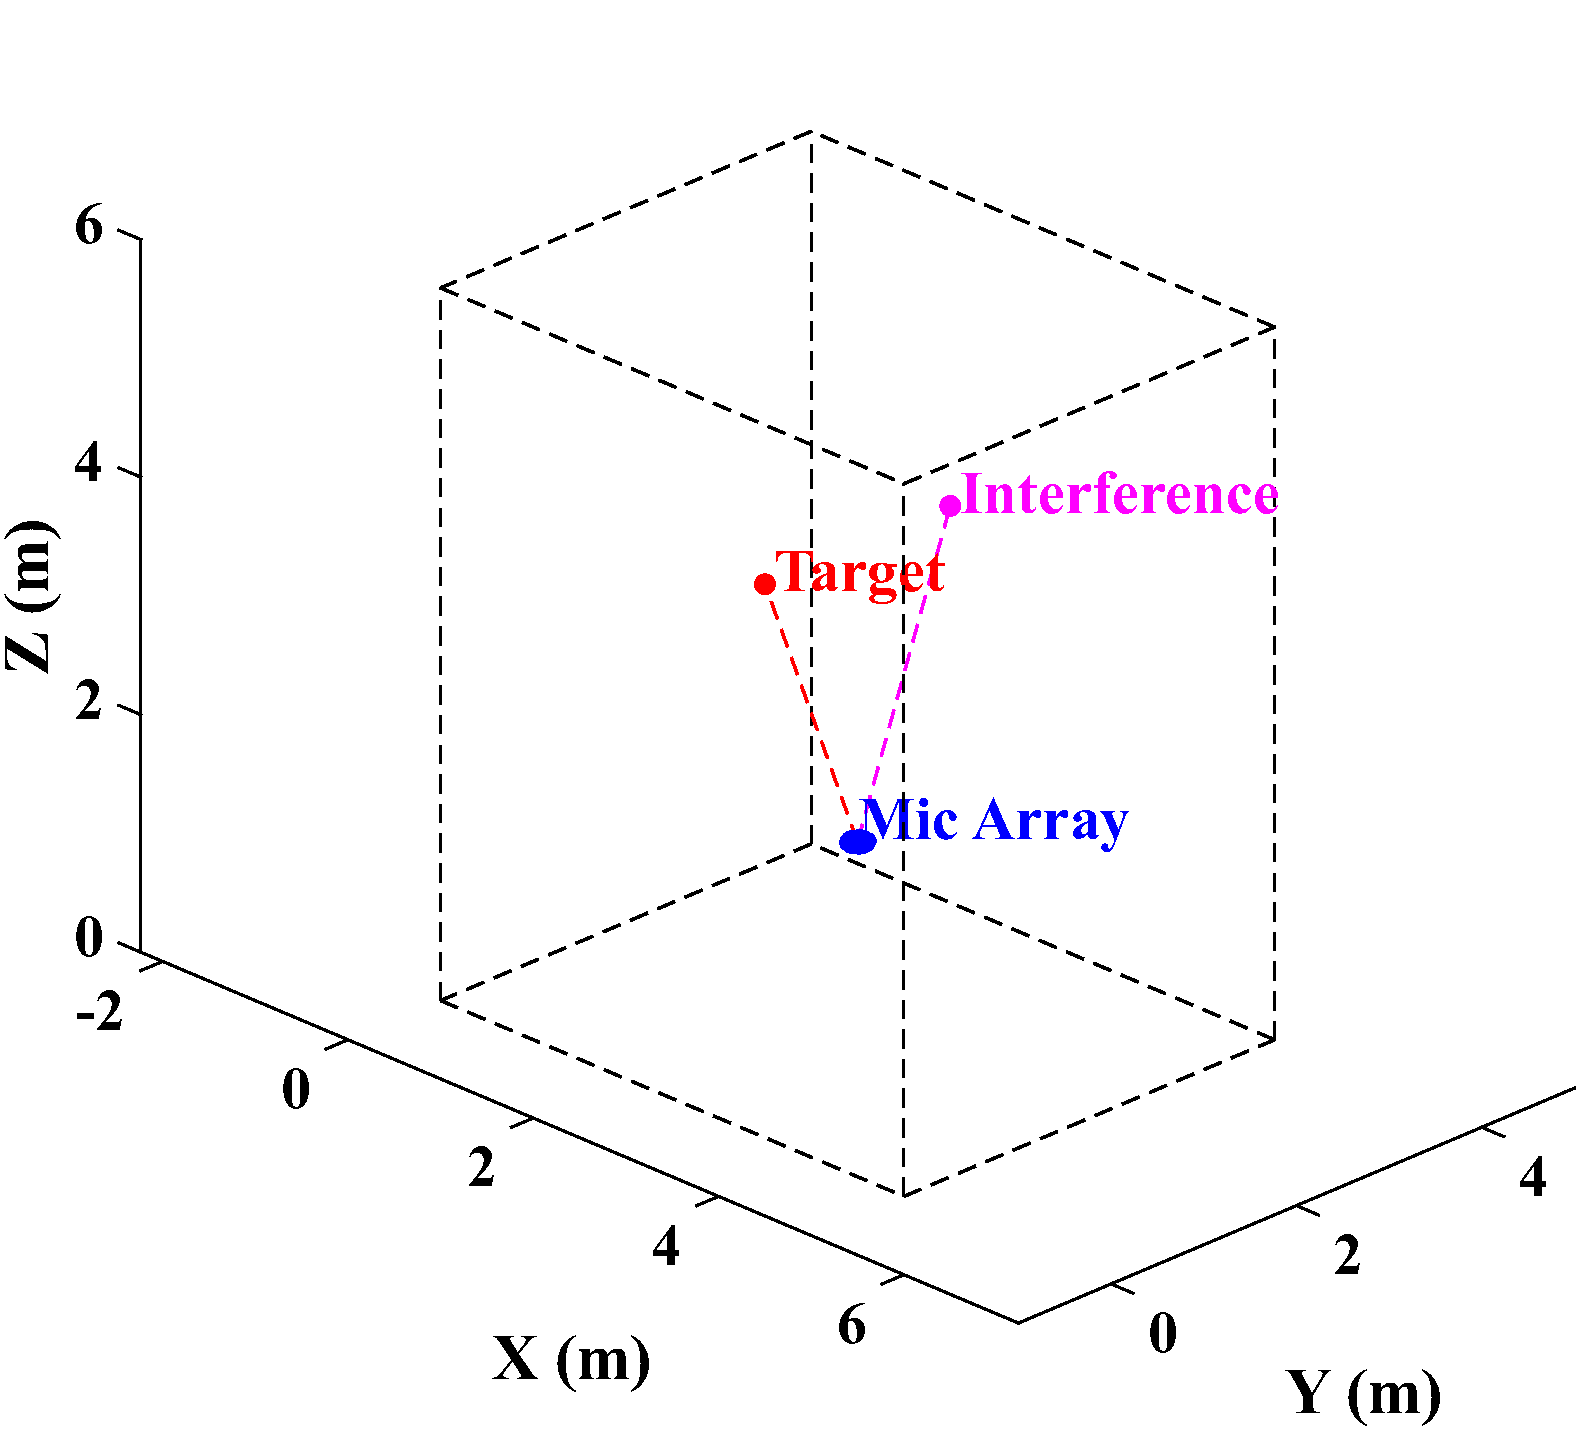
\includegraphics[width=0.8\linewidth]{output/demo_2k_4k/figures/Room_layout_with_sources_3d}
\caption{Room layout and microphone array configuration for RIR-based simulation.}
\label{fig:room_layout}
\end{figure}

The microphone array geometry and source positions are illustrated in a top-down view in Fig. \ref{fig:room_layout_2d}. This configuration allows for a comprehensive evaluation of the MVDR beamforming performance in enhancing the target signal while suppressing interference under realistic acoustic conditions.
\begin{figure}
\centering
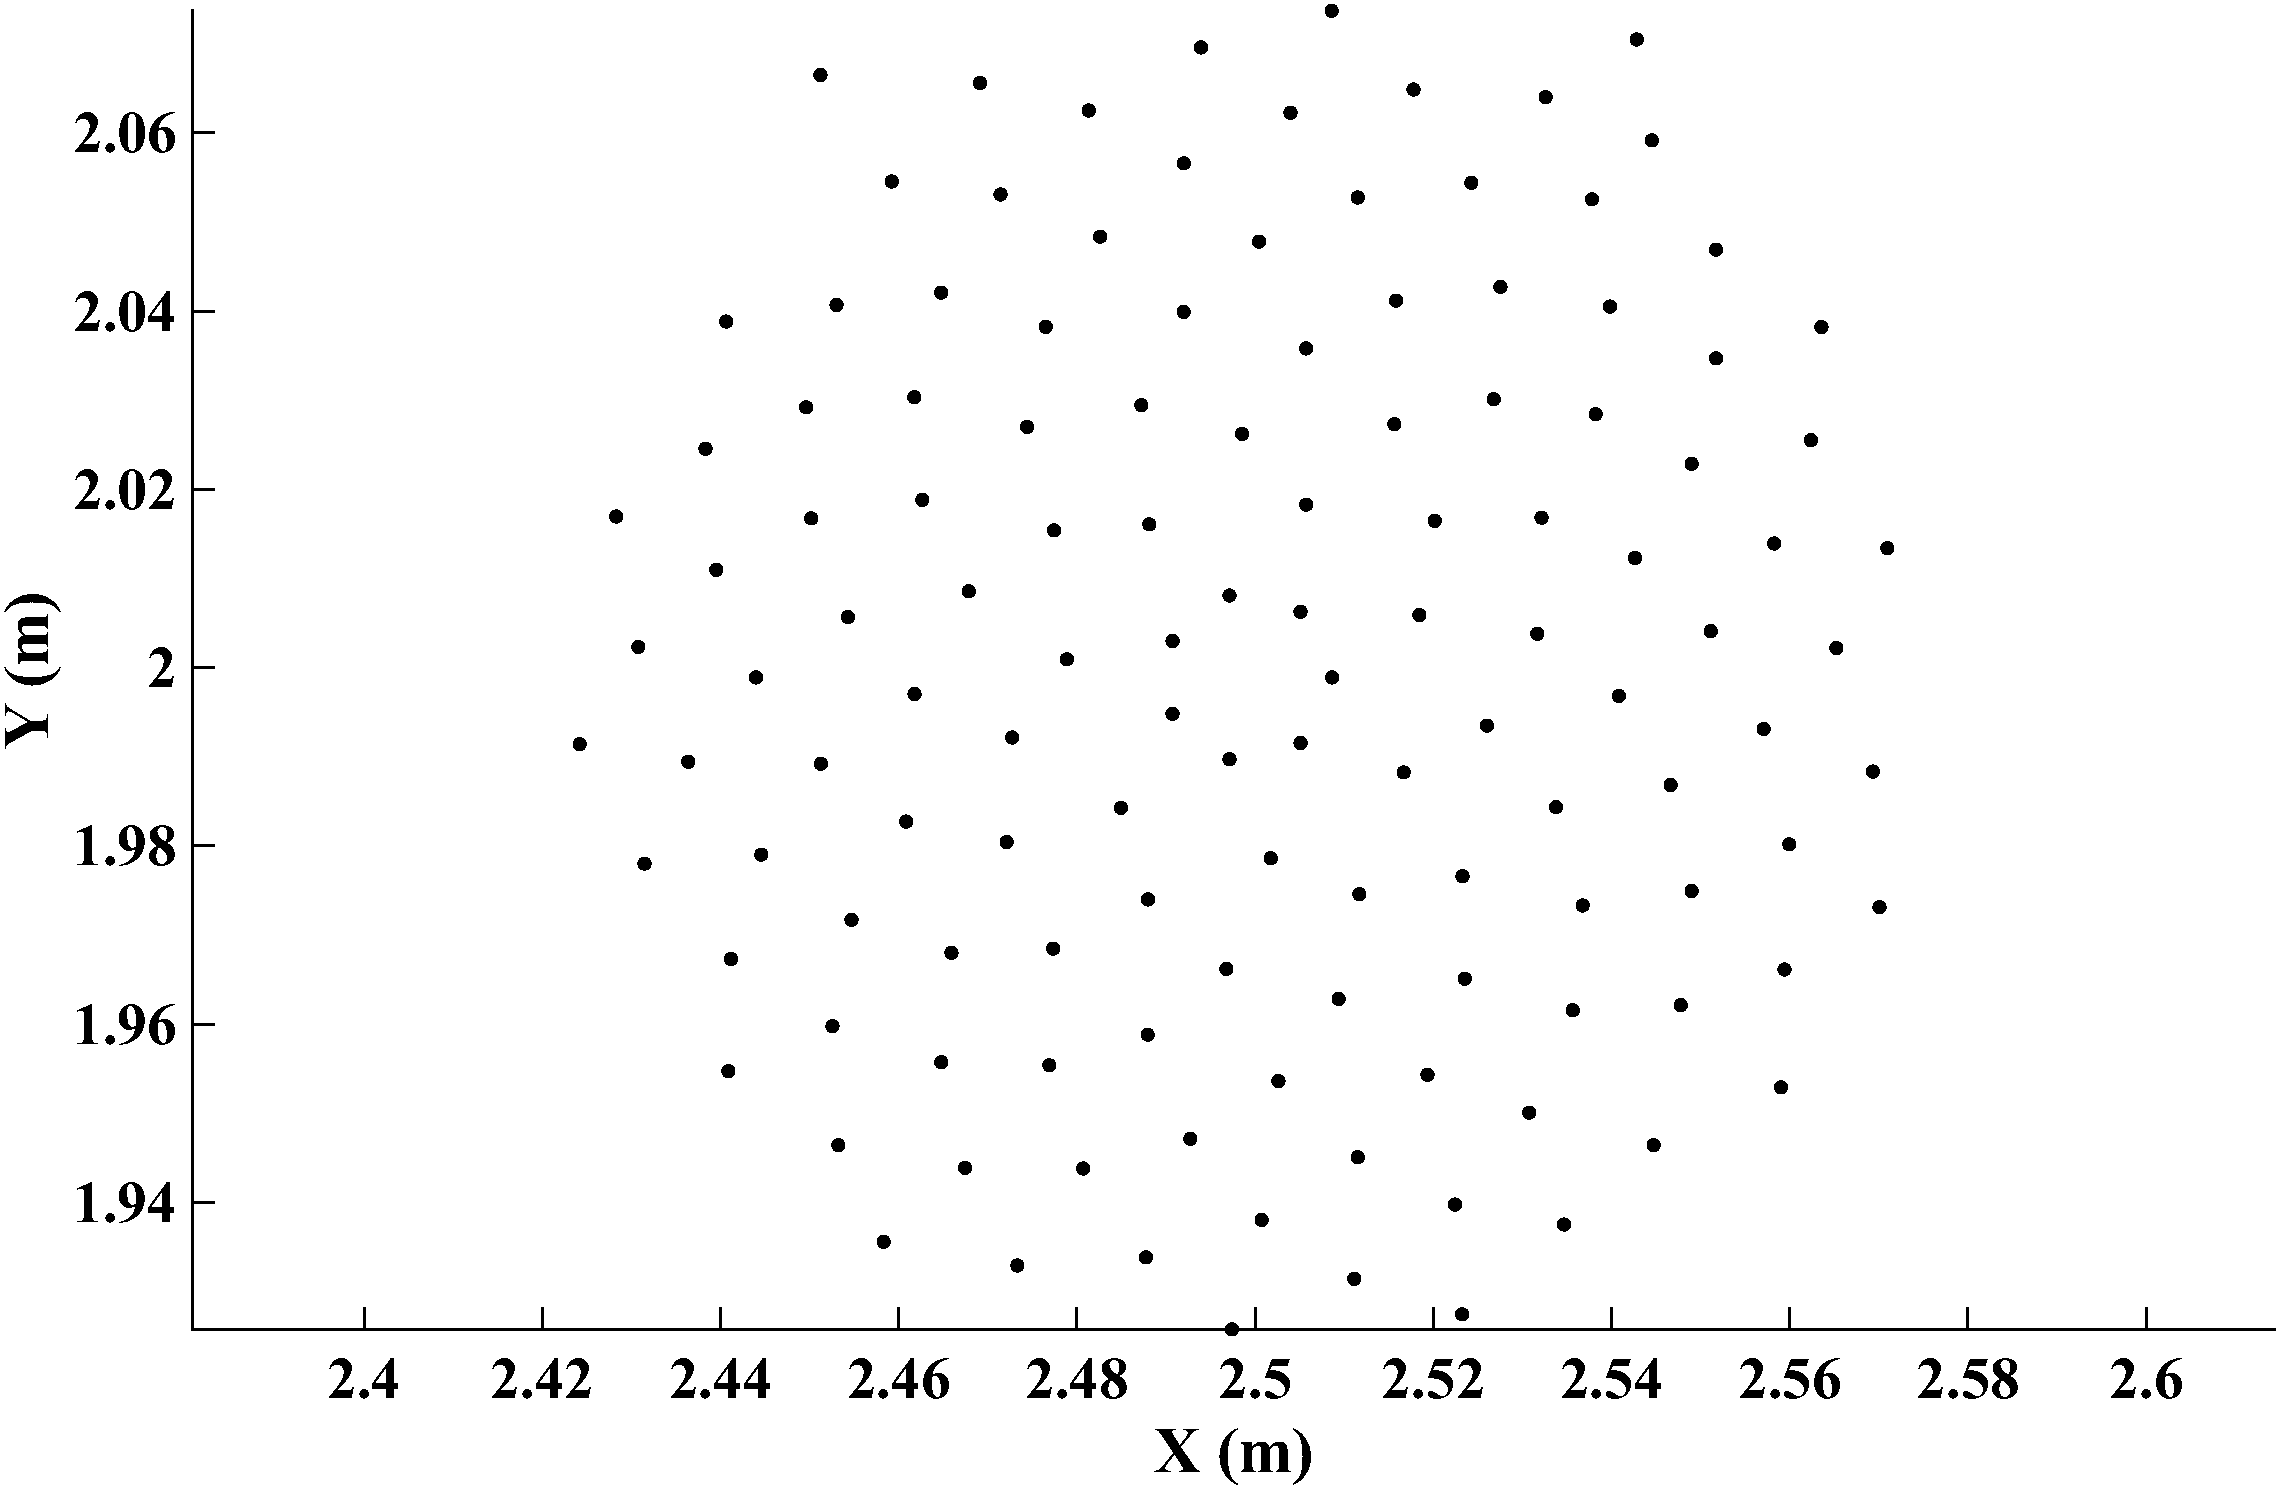
\includegraphics[width=0.8\linewidth]{output/demo_2k_4k/figures/Microphone_array_geometry_2d}
\caption{Top-down view of room layout and microphone array configuration.}
\label{fig:room_layout_2d}
\end{figure}

\subsection{Simulation 1:  Narrowband Sinusoid Signals}
A demo is conducted, where the target and interference signals are modeled as 2kHz and 4kHz narrowband sinusoids, respectively. These signals are convolved with their respective RIRs to generate multichannel received signals. No manual inter-channel delays or phase corrections are applied; all timing differences naturally arise from source-array geometric relationships and the RIR computation, ensuring consistency in physical modeling. 
\subsubsection{Power Spectral Density (PSD) Analysis}

The PSD shown that the target and interference signals have distinct spectral characteristics, with the target signal concentrated around 2 kHz and the interference signal around 4 kHz, as illustrated in the Power Spectral Density (PSD) plot in Fig. \ref{fig:signal_configuration}. This setup allows for a clear evaluation of the MVDR beamforming performance in suppressing the interference while preserving the target signal across the frequency spectrum.

\begin{figure}
\centering
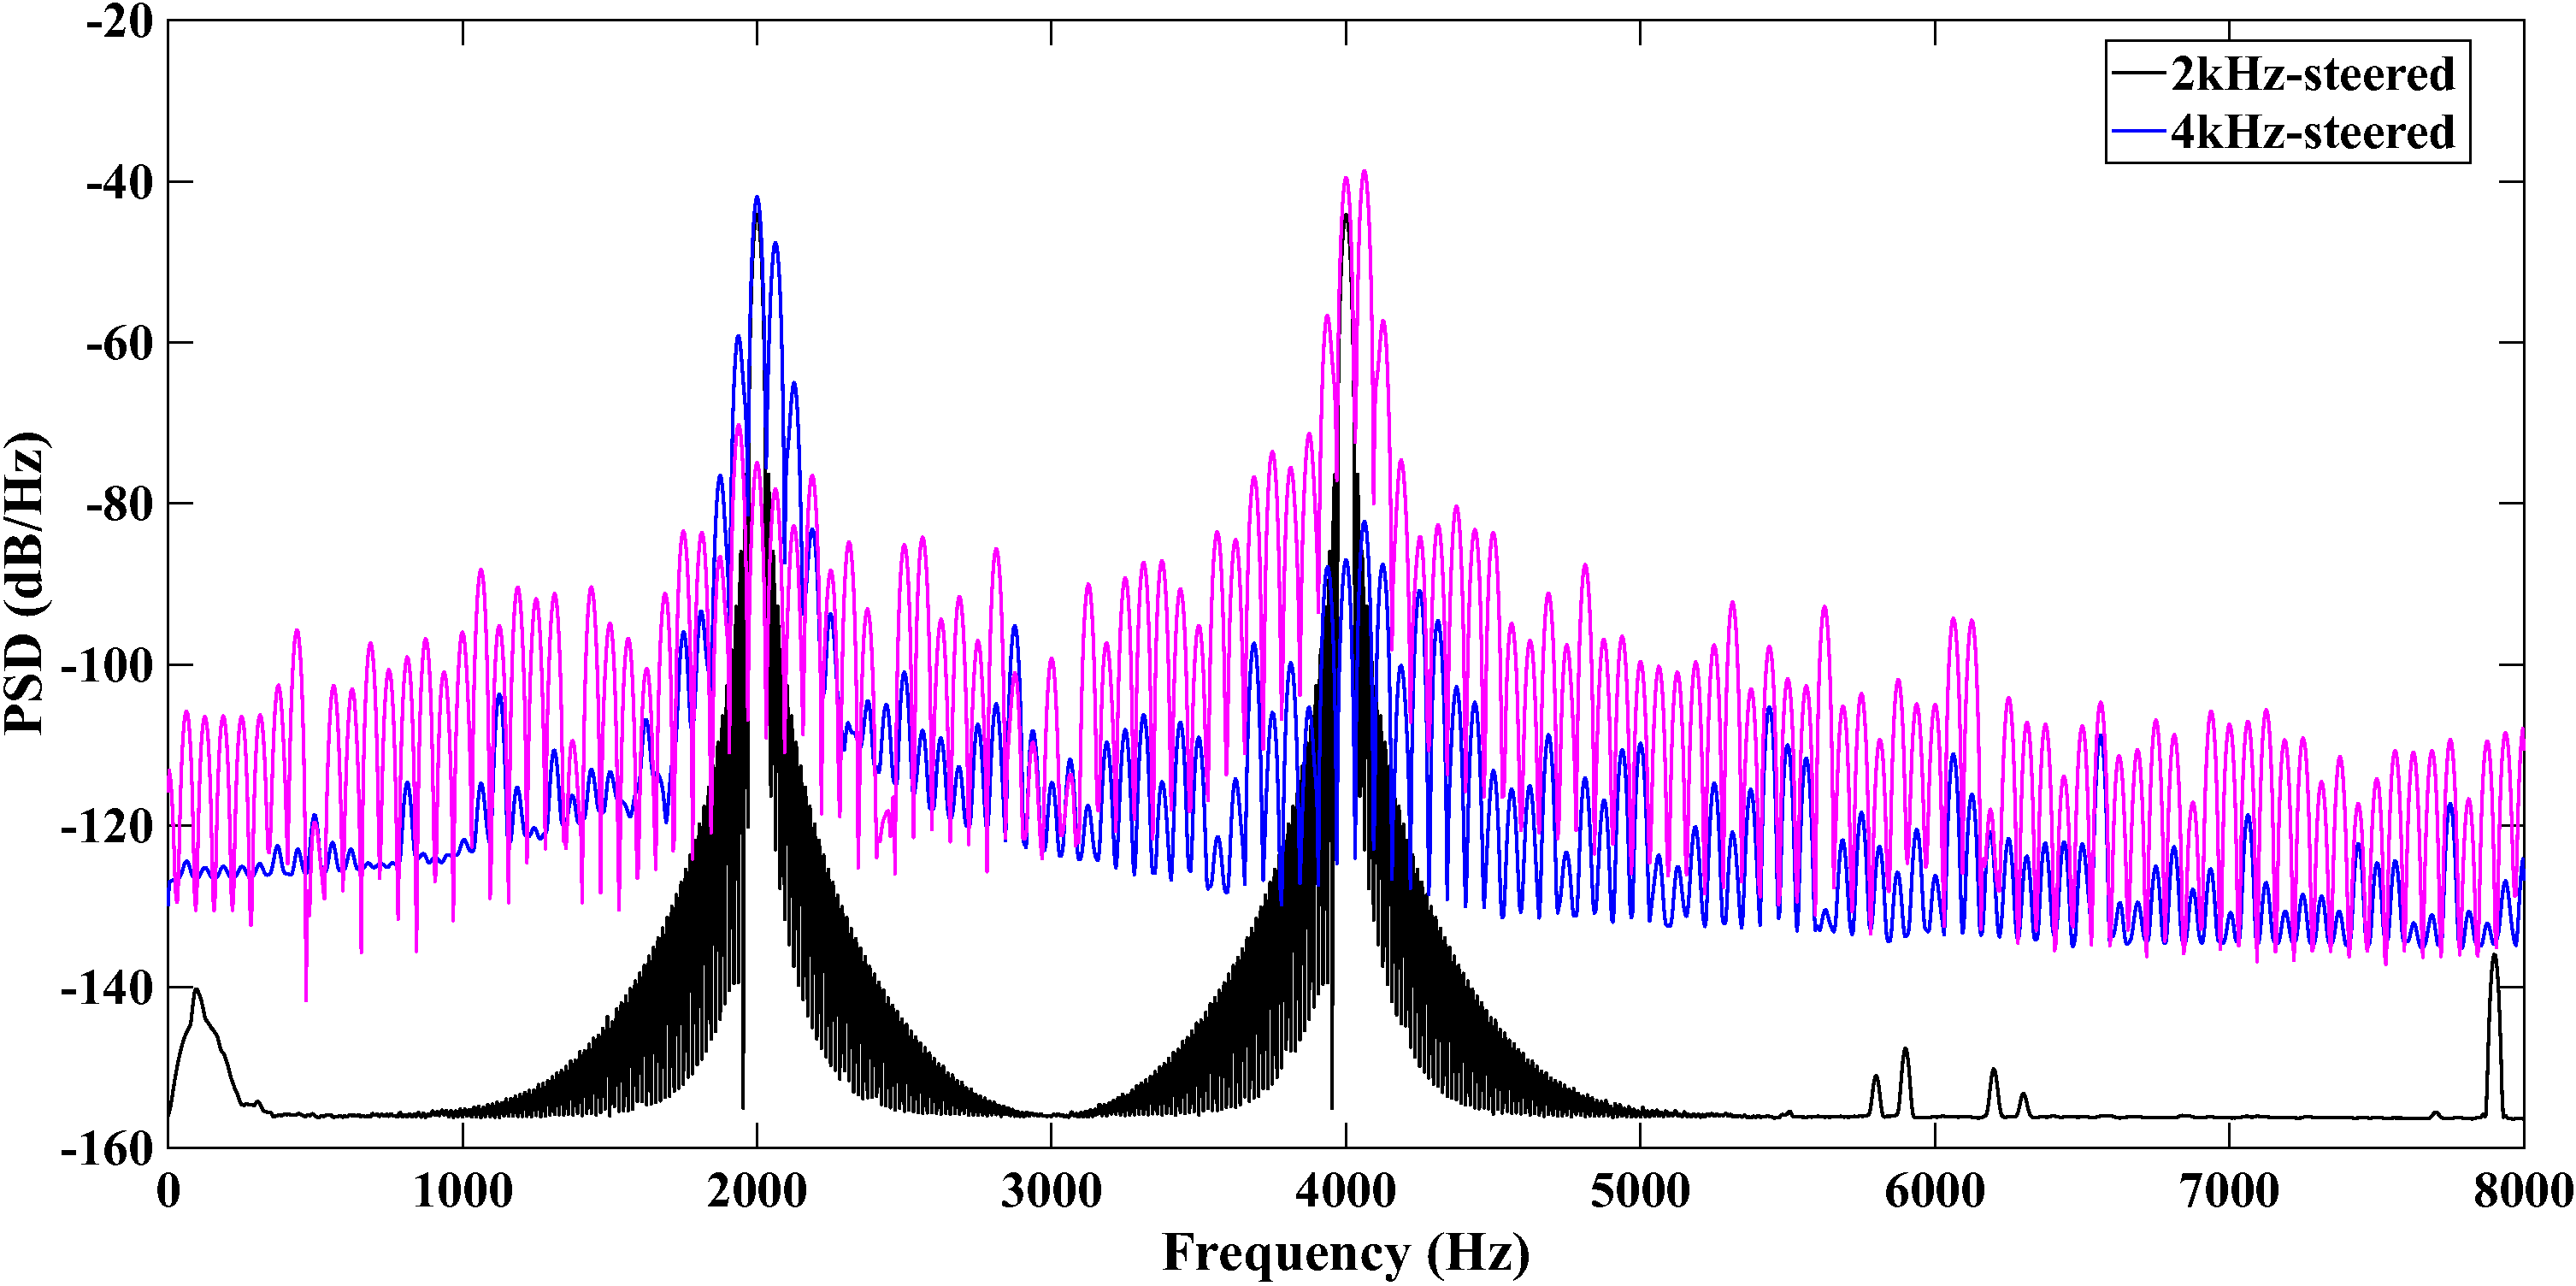
\includegraphics[width=1\linewidth]{output/demo_2k_4k/figures/PSD_fullband}
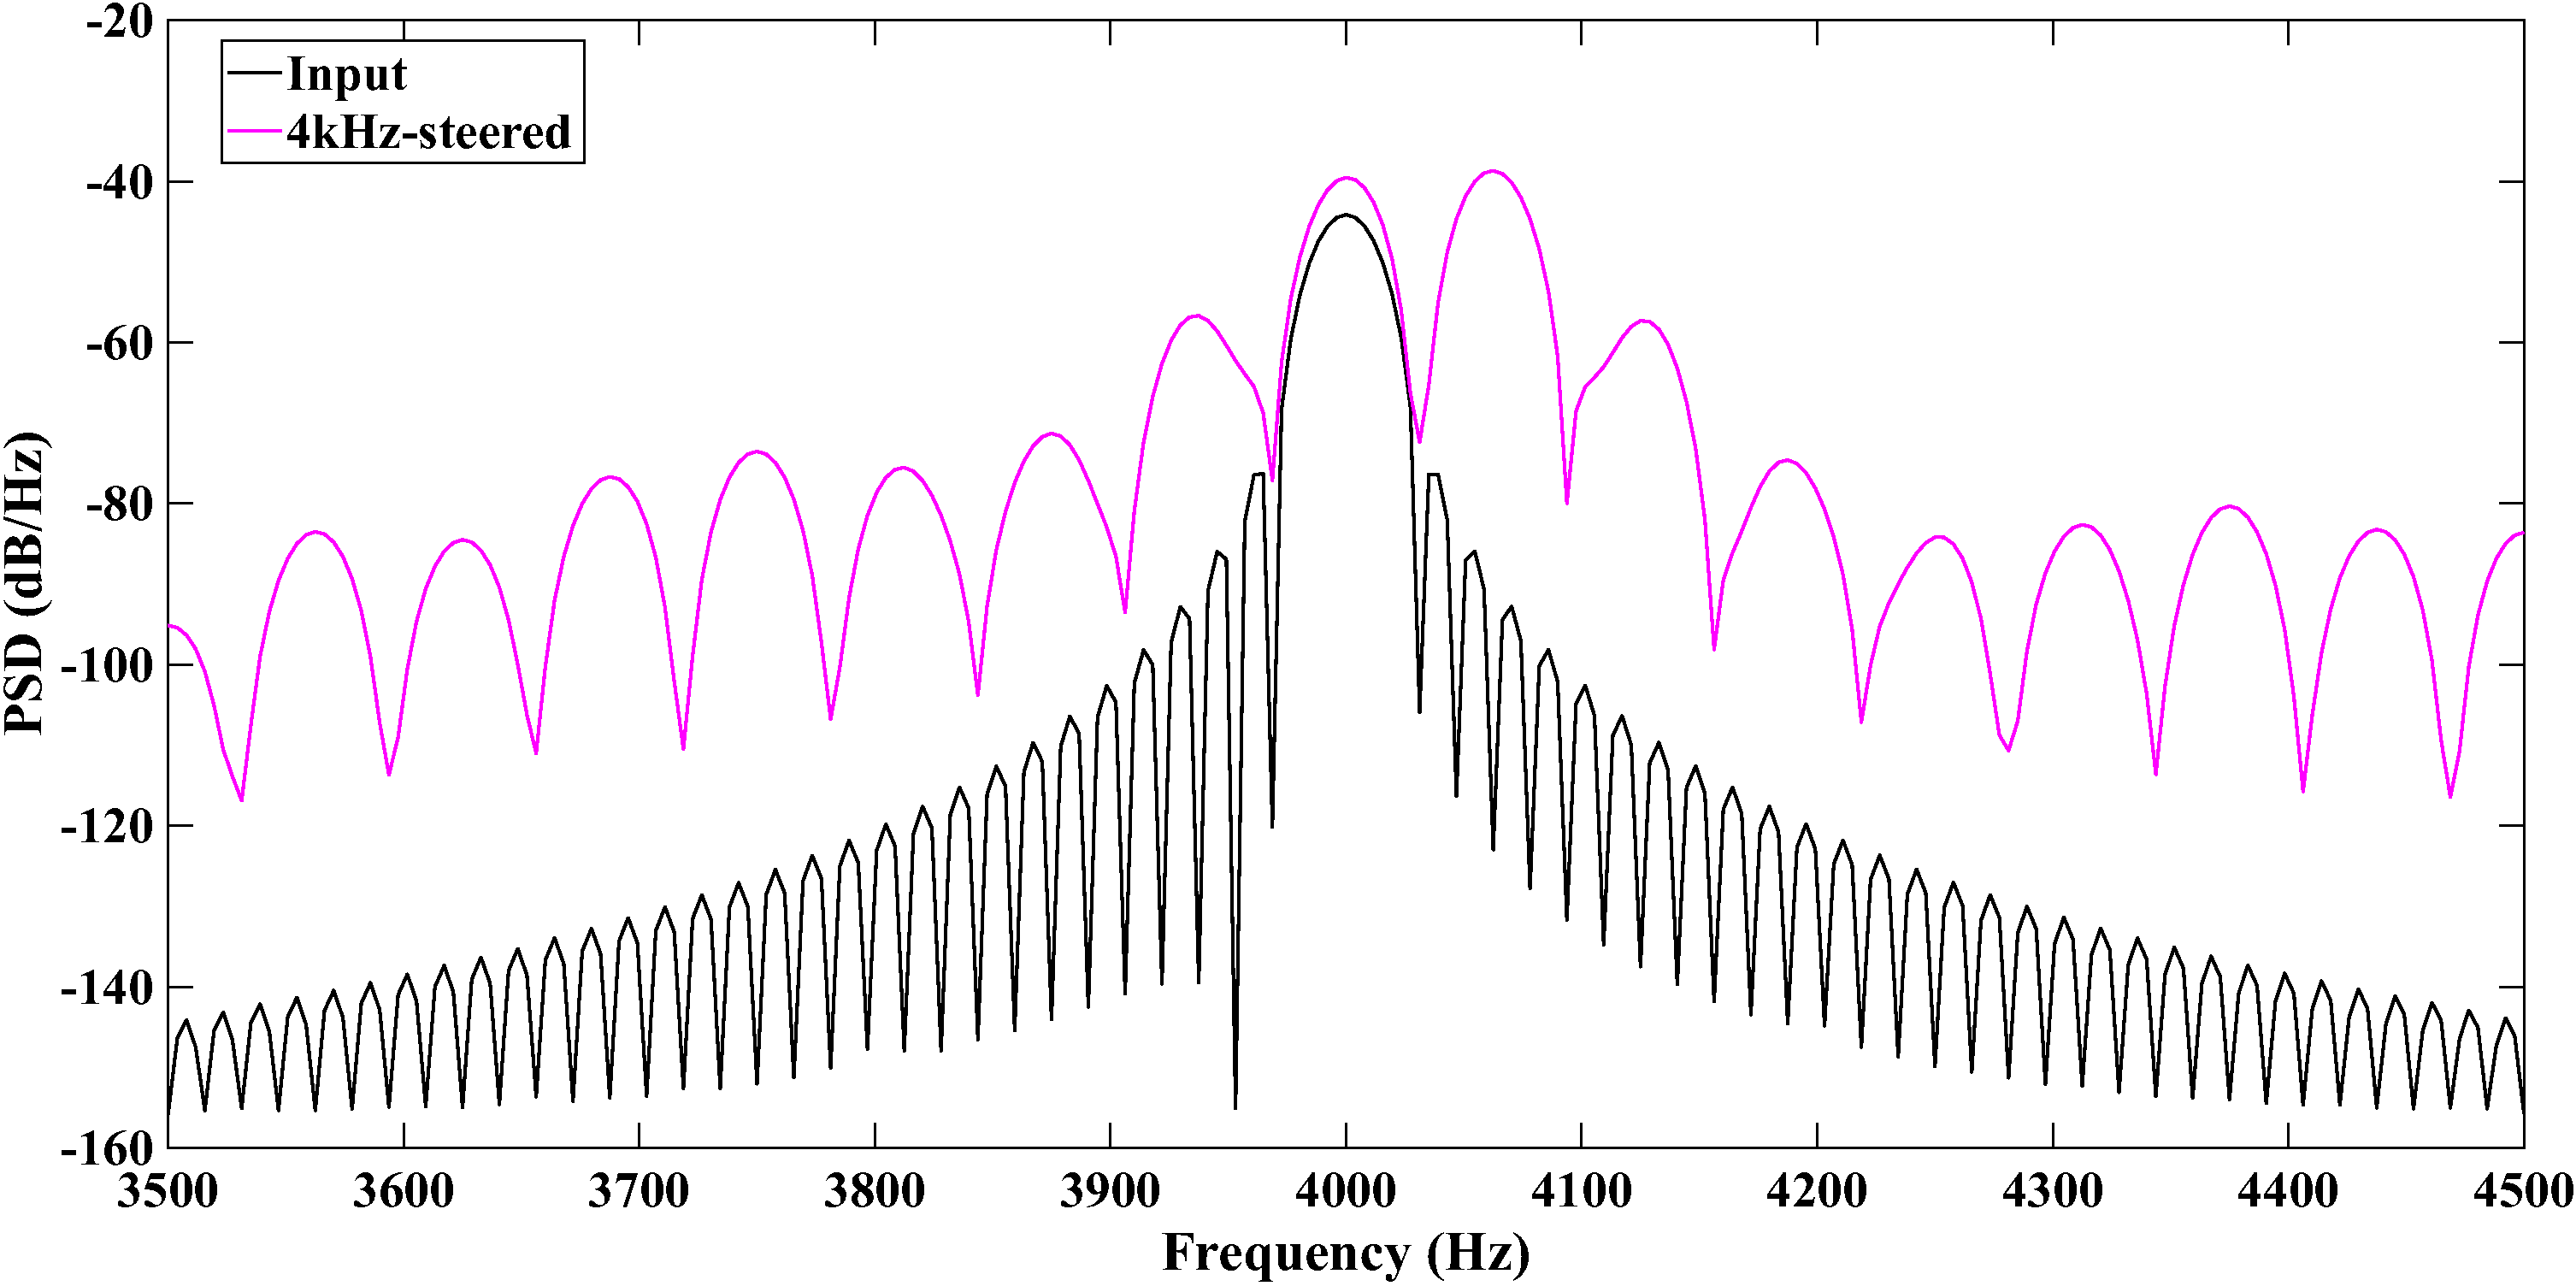
\includegraphics[width=1\linewidth]{output/demo_2k_4k/figures/PSD_4kHz}
\caption{Power Spectral Density (PSD) of the target and interference signals after RIR convolution. We steered the target to the 2kHz and 4kHz signal, respectively.}
\label{fig:signal_configuration}

\end{figure}

\subsubsection{Eigenvalue Spectrum Analysis}

As shown in Fig. \ref{fig:eigenvalue_spectrum}, the eigenvalue spectrum of the covariance matrix at the 2 kHz frequency bin reveals a significant gap between the largest eigenvalue and the remaining eigenvalues. This indicates a strong spatial structure in the received signals, with the target signal dominating the spatial subspace. The presence of this gap suggests that the MVDR beamforming algorithm can effectively exploit the spatial information to enhance the target signal while suppressing interference, providing stable conditions for accurate weight computation.
\begin{figure}
\centering
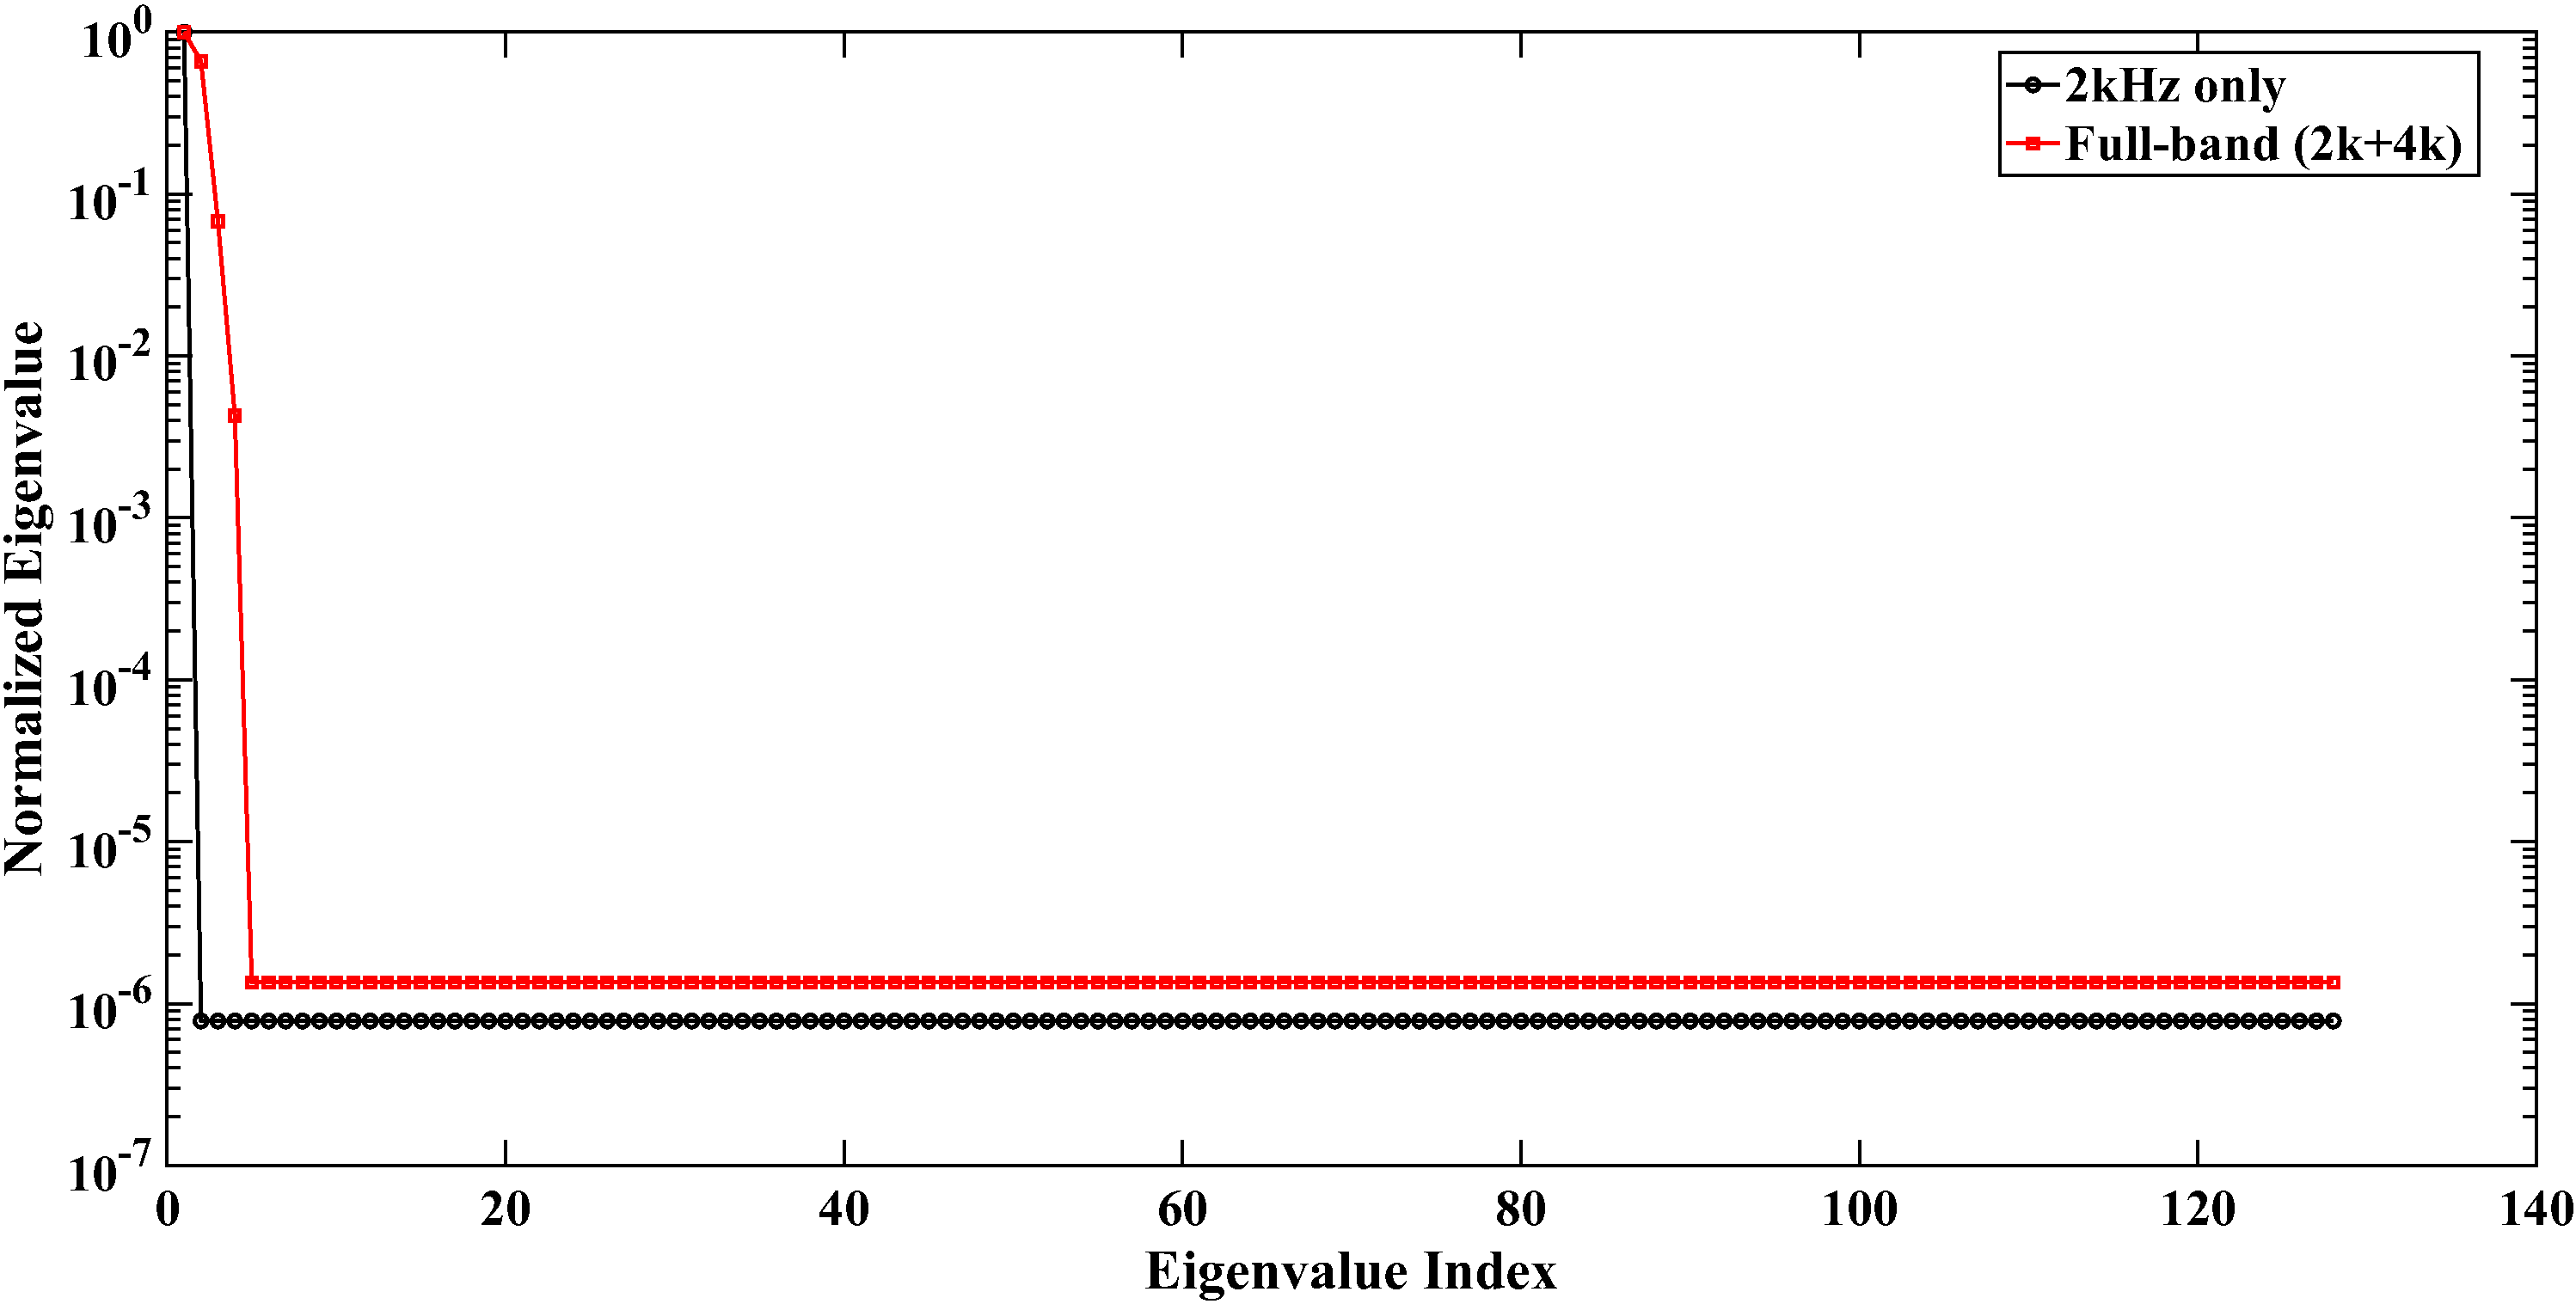
\includegraphics[width=1\linewidth]{output/demo_2k_4k/figures/Eigenspectrum_comparison_2kHz_vs_fullband}
\caption{Eigenvalue spectrum of the covariance matrix at the 2 kHz frequency bin. The significant gap between the largest eigenvalue and the others indicates a strong spatial structure, favorable for MVDR beamforming performance.}
\label{fig:eigenvalue_spectrum}
\end{figure}


The eigenvalue decomposition of the received signal covariance matrix reveals the underlying signal subspace structure. As shown in Fig. \ref{fig:Eigenvalue_detailed_analysis}, the spectrum 
exhibits three dominant eigenvalues that exceed the 1\% significance threshold, corresponding to: (1) the primary target signal component ($\lambda_1 = 0.1346$), (2) the interference component ($\lambda_2 = 0.0886$), and (3) a secondary component attributed to reverberation or multipath effects 
($\lambda_3 = 0.0091$). The remaining eigenvalues ($\lambda_4 - \lambda_n \approx 10^{-7}$) represent the 
noise floor. By restricting the MVDR signal subspace to M = 2 principal eigenvalues, the proposed method effectively suppresses the reverberation component while preserving the target and interference spatial signatures, resulting in a well-conditioned inverse covariance matrix.


\begin{figure}
\centering
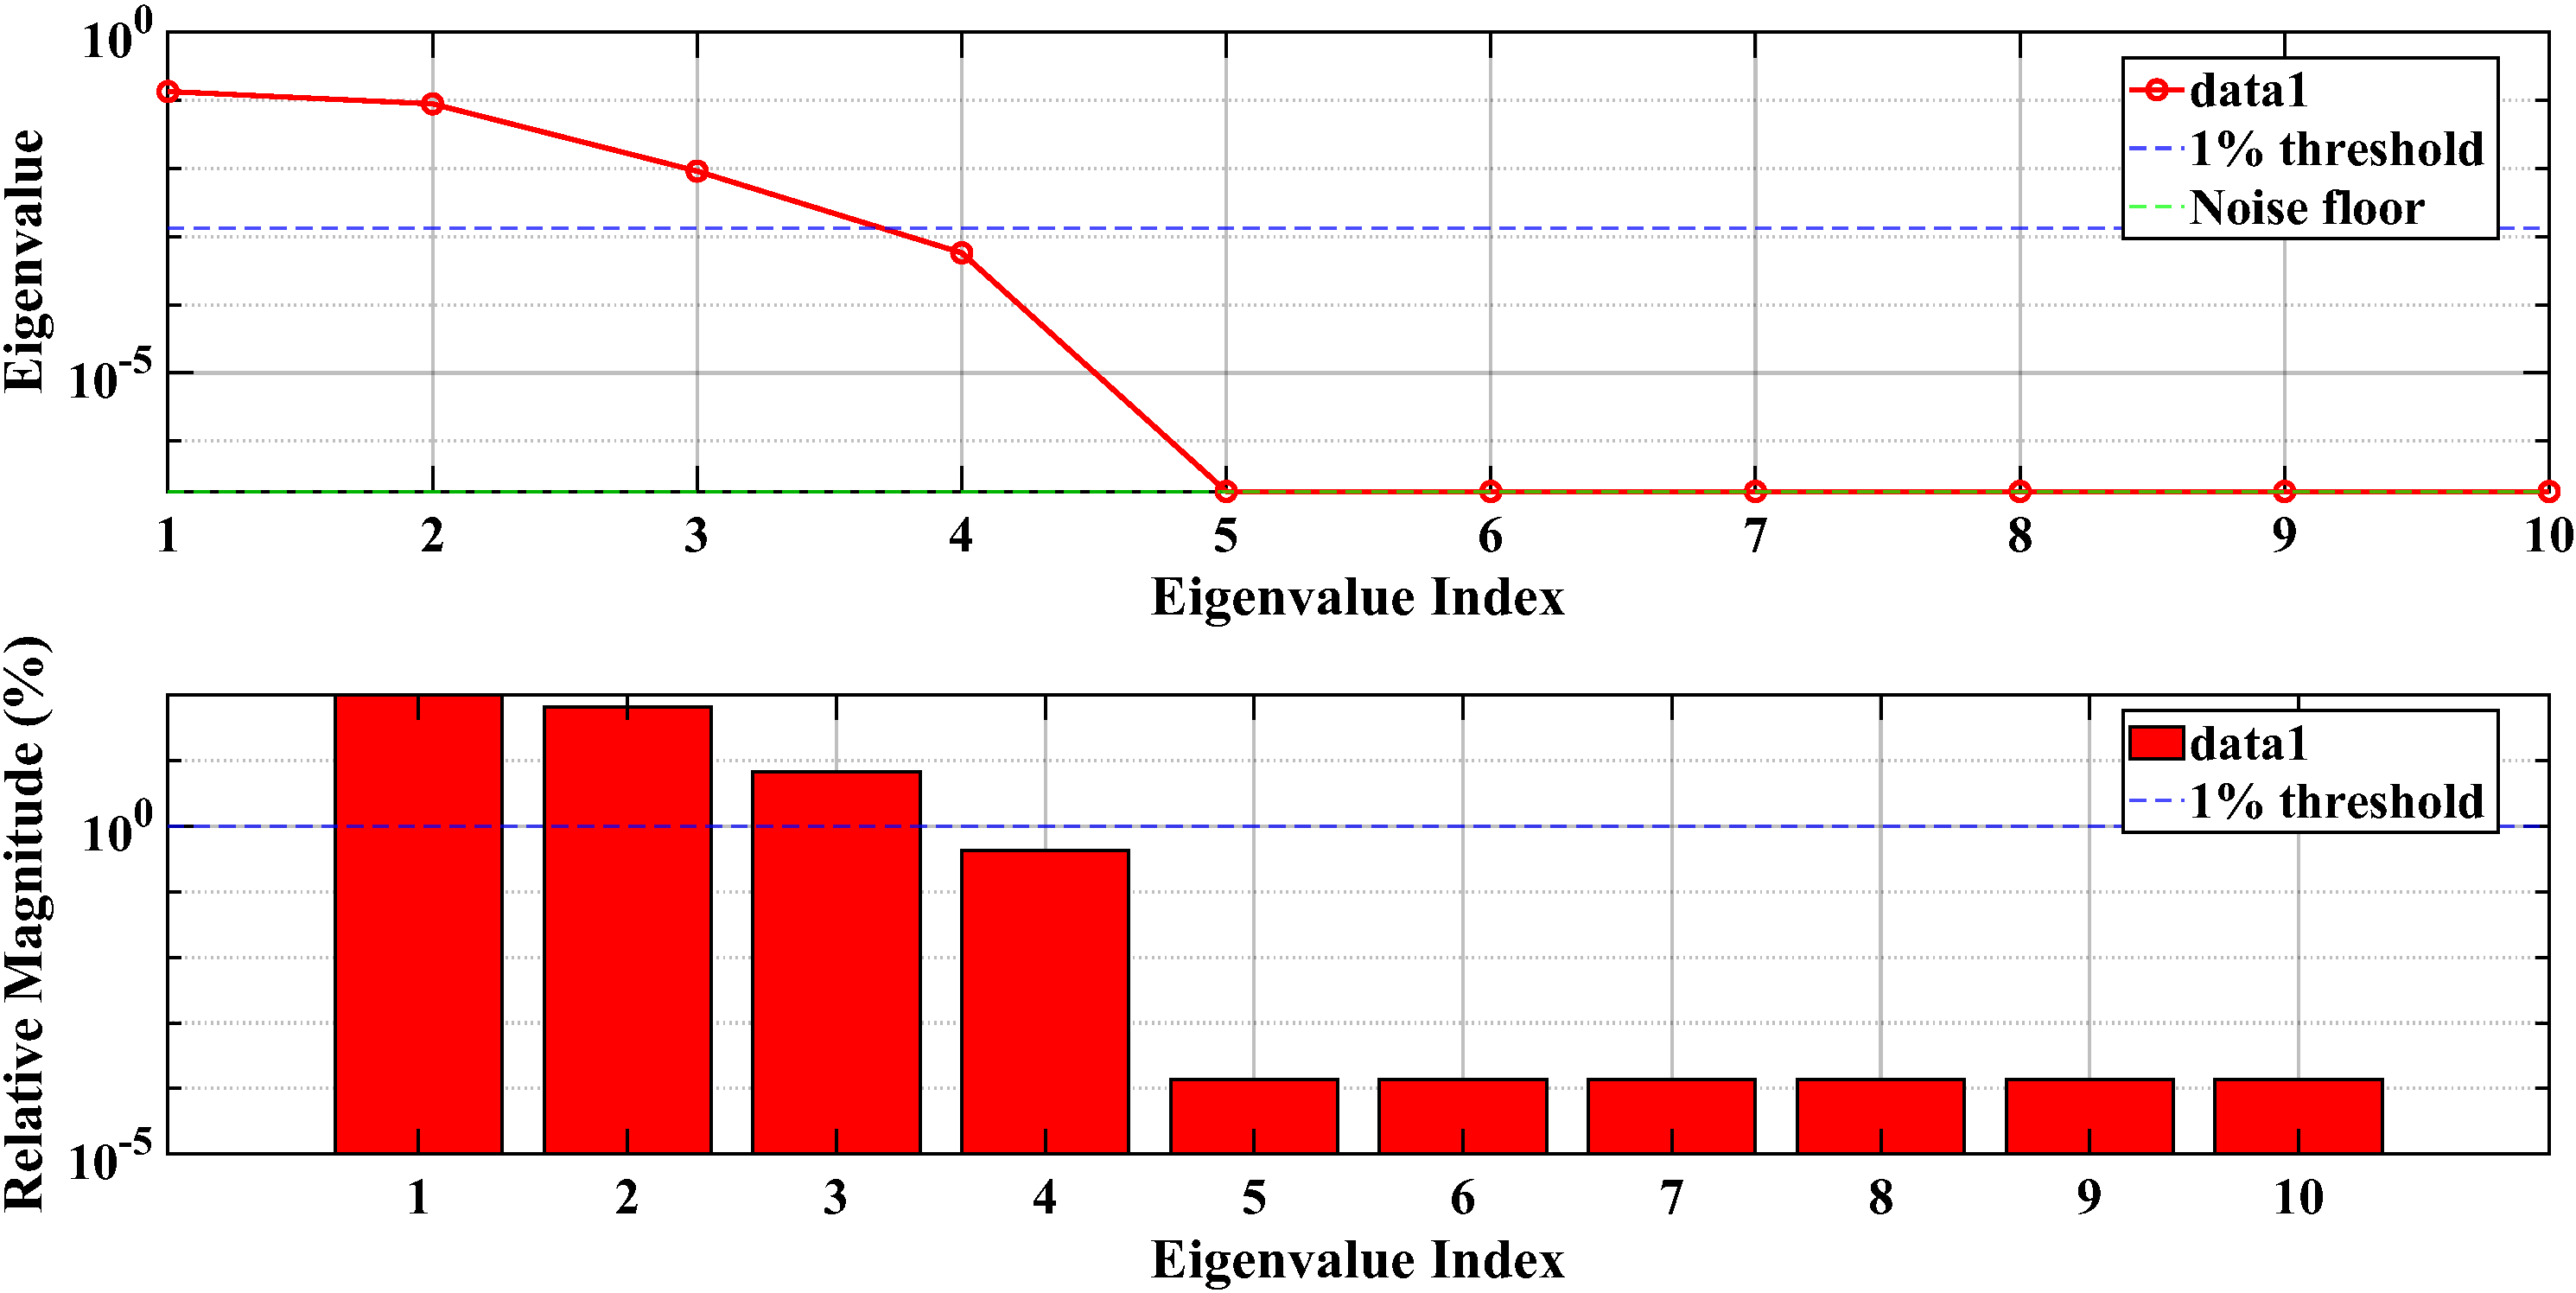
\includegraphics[width=1\linewidth]{output/demo_2k_4k/figures/Eigenvalue_detailed_analysis}
\caption{Eigenvalue spectrum of the full-band (2 kHz + 4 kHz) covariance matrix (top) showing normalized eigenvalue magnitudes on logarithmic scale with the 1\% threshold for signal source detection. (Bottom) Relative eigenvalue 
magnitudes (\%) on logarithmic scale indicating three eigenvalues exceeding the 1\% threshold ($\lambda_1 = 13.46\%$, $\lambda_2 = 8.86\%$, $\lambda_3 = 0.91\%$), corresponding to target signal, interference, and reverberation/noise subspace, respectively. The sharp drop at index 4-5 identifies the signal-to-noise transition boundary.}
\label{fig:Eigenvalue_detailed_analysis}
\end{figure}

\subsubsection{Multi-parameter Eigenvalue Analysis}
To characterize the MVDR beamformer's performance across acoustic conditions, we systematically analyze eigenvalue distributions and performance metrics as functions of the room wall reflection coefficient $\beta$.



As shown in Fig. \ref{multi_beta_comparison},the eigenvalue distribution exhibits significant dependence on the wall reflection coefficient $\beta$. In the anechoic case ($\beta = 0$), a clear separation exists between the dominant eigenvalues ($\lambda_1 \approx \lambda_2$) associated with the signal subspace and the noise floor. However, as $\beta$ increases to 0.8, the eigenvalue curve flattens progressively, indicating increased multipath coupling and reduced signal-to-subspace-noise ratio.


\begin{figure}
\centering
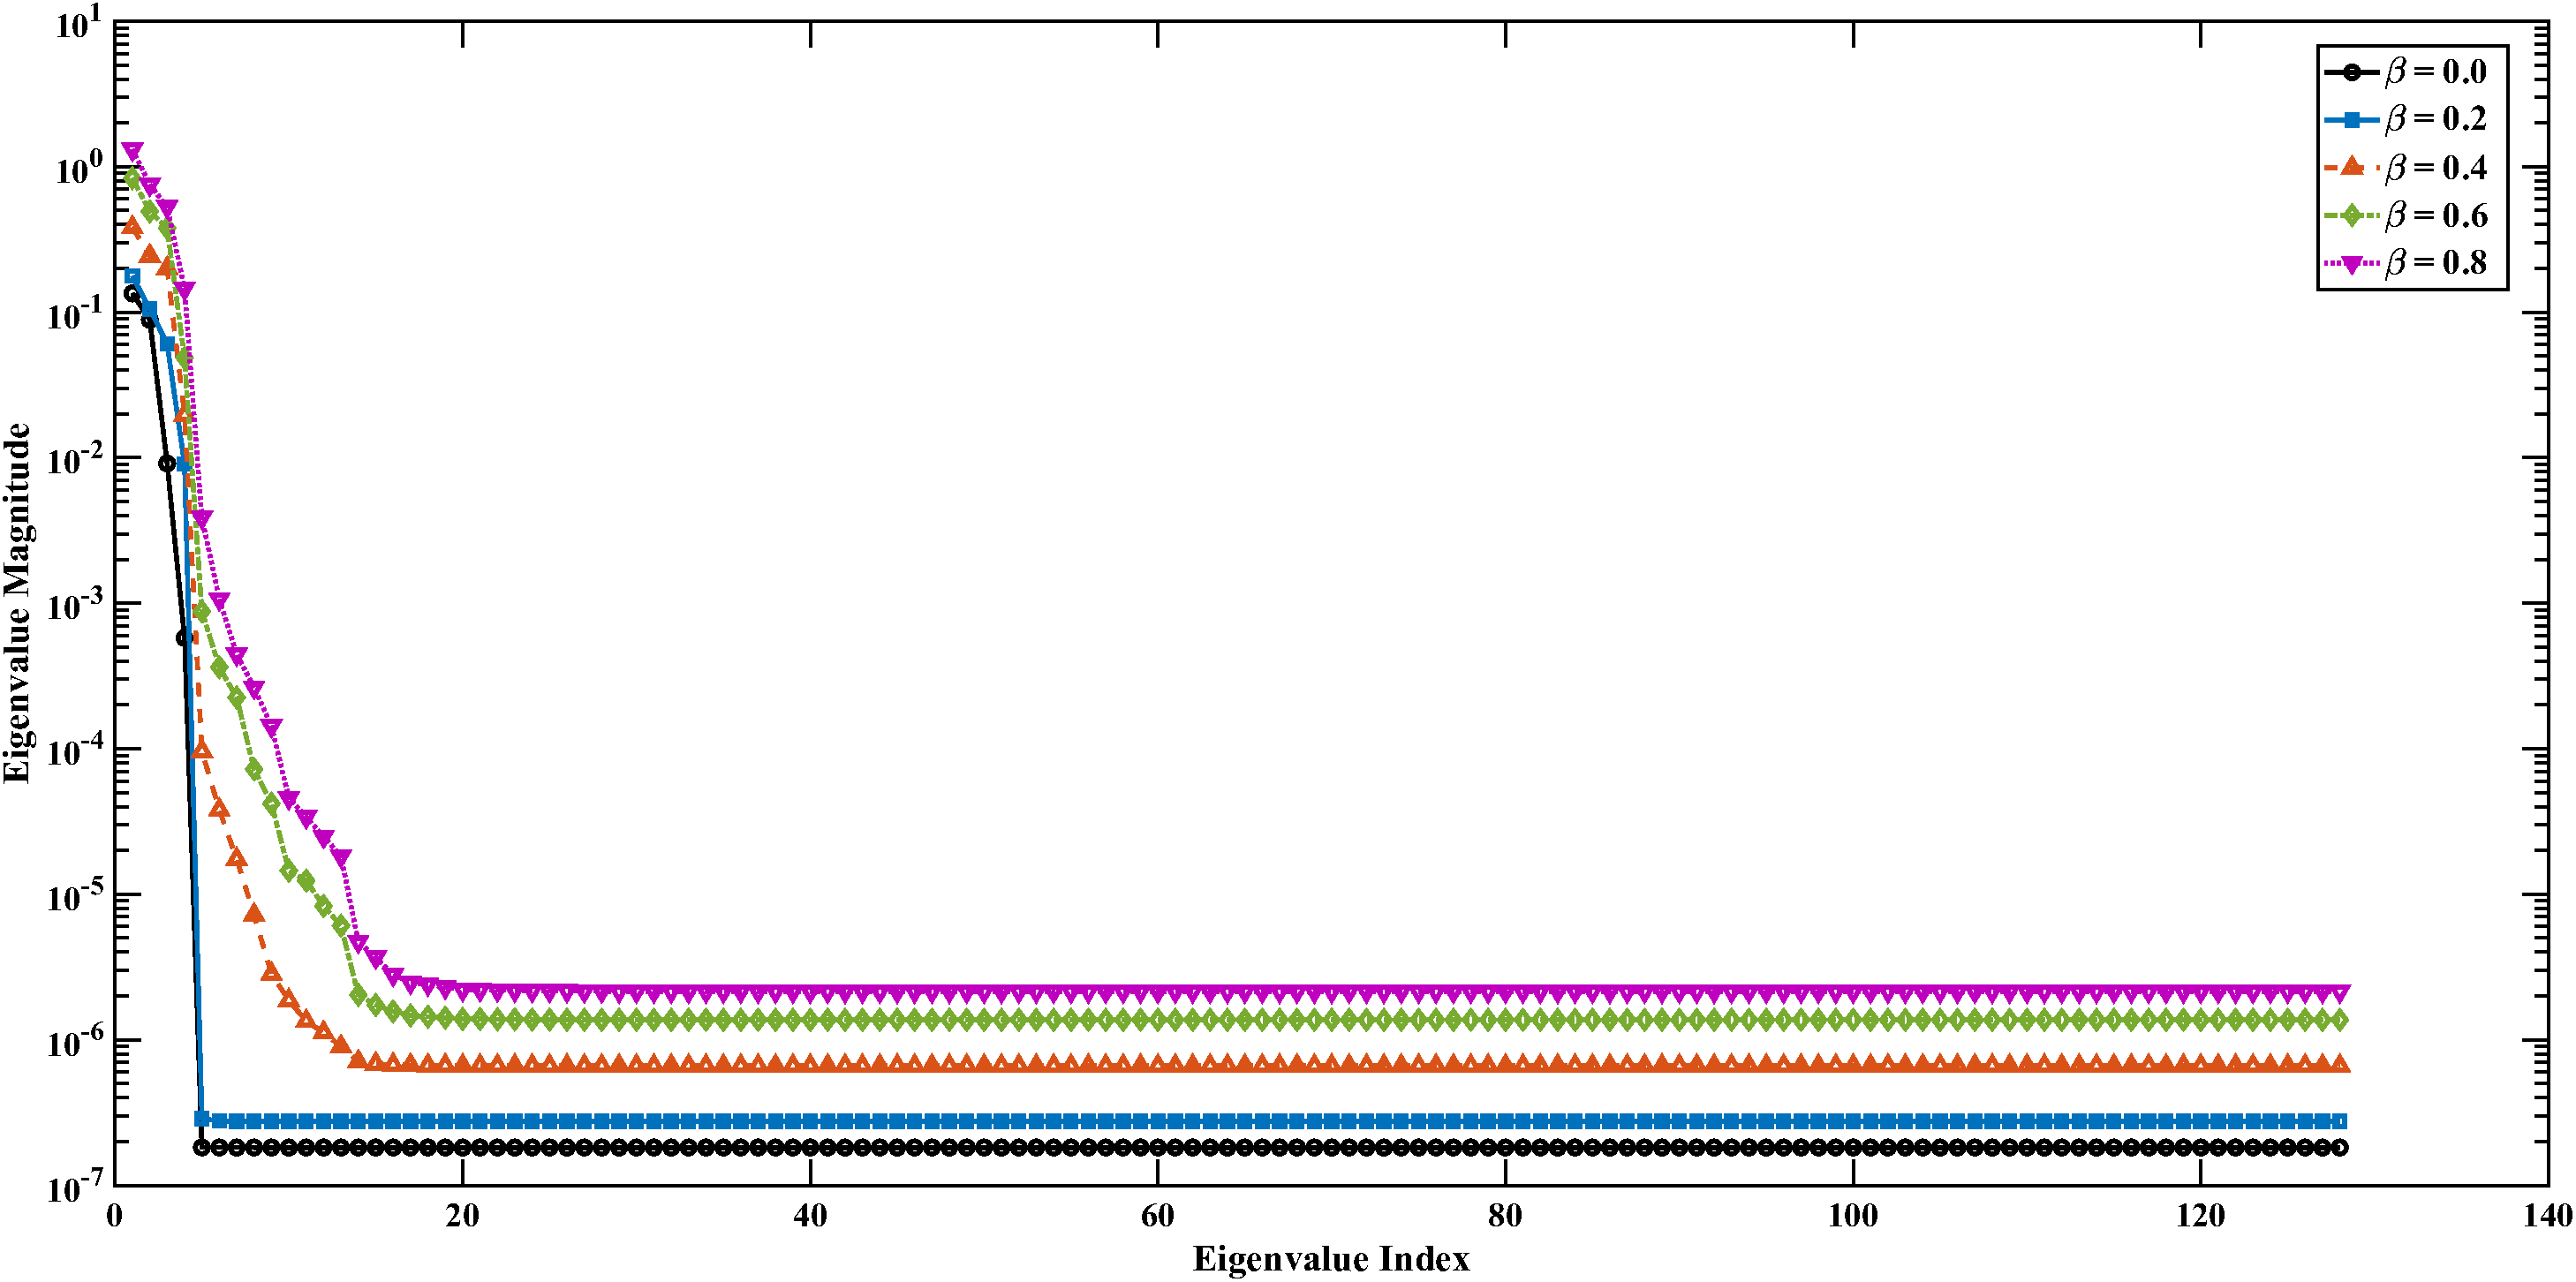
\includegraphics[width=1\linewidth]{output/demo_2k_4k/multi_beta_comparison/Eigenspectra_fullband_comparison}
\caption{Covariance eigenspectra of the composite received signal as functions of wall reflection coefficient $\beta$. Eigenvalues are regularized with diagonal loading. The curves demonstrate the progressive deterioration of signal-to-noise eigenvalue separation with increasing room reverberation.}
\label{multi_beta_comparison}
\end{figure}


The performance metrics presented in Fig. \ref{Performance_metrics_vs_beta} characterize the MVDR beamformer's effectiveness across a range of acoustic environments. Fig. \ref{Performance_metrics_vs_beta}(a) demonstrates that the target-steered configuration achieves SNR improvements exceeding 15 dB in low-reverberation conditions, degrading gracefully to approximately 7 dB at high reflection coefficients. This degradation is primarily attributed to multipath decorrelation of the signal steering vector, which violates the assumptions underlying MVDR's optimal performance.

The condition number evolution presented in Fig. \ref{Performance_metrics_vs_beta}(c) provides critical insight into the numerical stability requirements across the parameter space. The exponential growth of $\kappa$ from approximately 700 (anechoic) to over 600,000 (highly reverberant) necessitates adaptive diagonal loading strategies. Specifically, the regularization parameter $\epsilon$ must be increased from $10^{-4}$ to $10^{-2}$ to maintain weight vector stability, as determined empirically through singular value inspection.


The interplay between SNR gain and condition number, illustrated in Fig. \ref{Performance_metrics_vs_beta}(a) and (c), reveals the fundamental trade-off in beamformer design. Aggressive regularization required for numerical stability introduces biasing that reduces adaptive suppression capability. This compromise between adaptation and robustness becomes increasingly critical as reverberation intensity increases, suggesting that fixed MVDR configurations are insufficient for deployment in highly reverberant venues.


Fig. \ref{Performance_metrics_vs_beta}(b) shows that interference-steered branch achieves complementary performance characteristics, with ISR gains (defined as output ISR minus input ISR) demonstrating less monotonic behavior than SNR gains. This non-monotonic pattern reflects the complex interaction between the target's multipath structure and the interference suppression objective, where increased diffuse reverberation can occasionally enhance interference suppression by reducing spatial coherence of unwanted signals. The values are summarized in Table \ref{tab:beta_performance}.

\begin{figure}
\centering
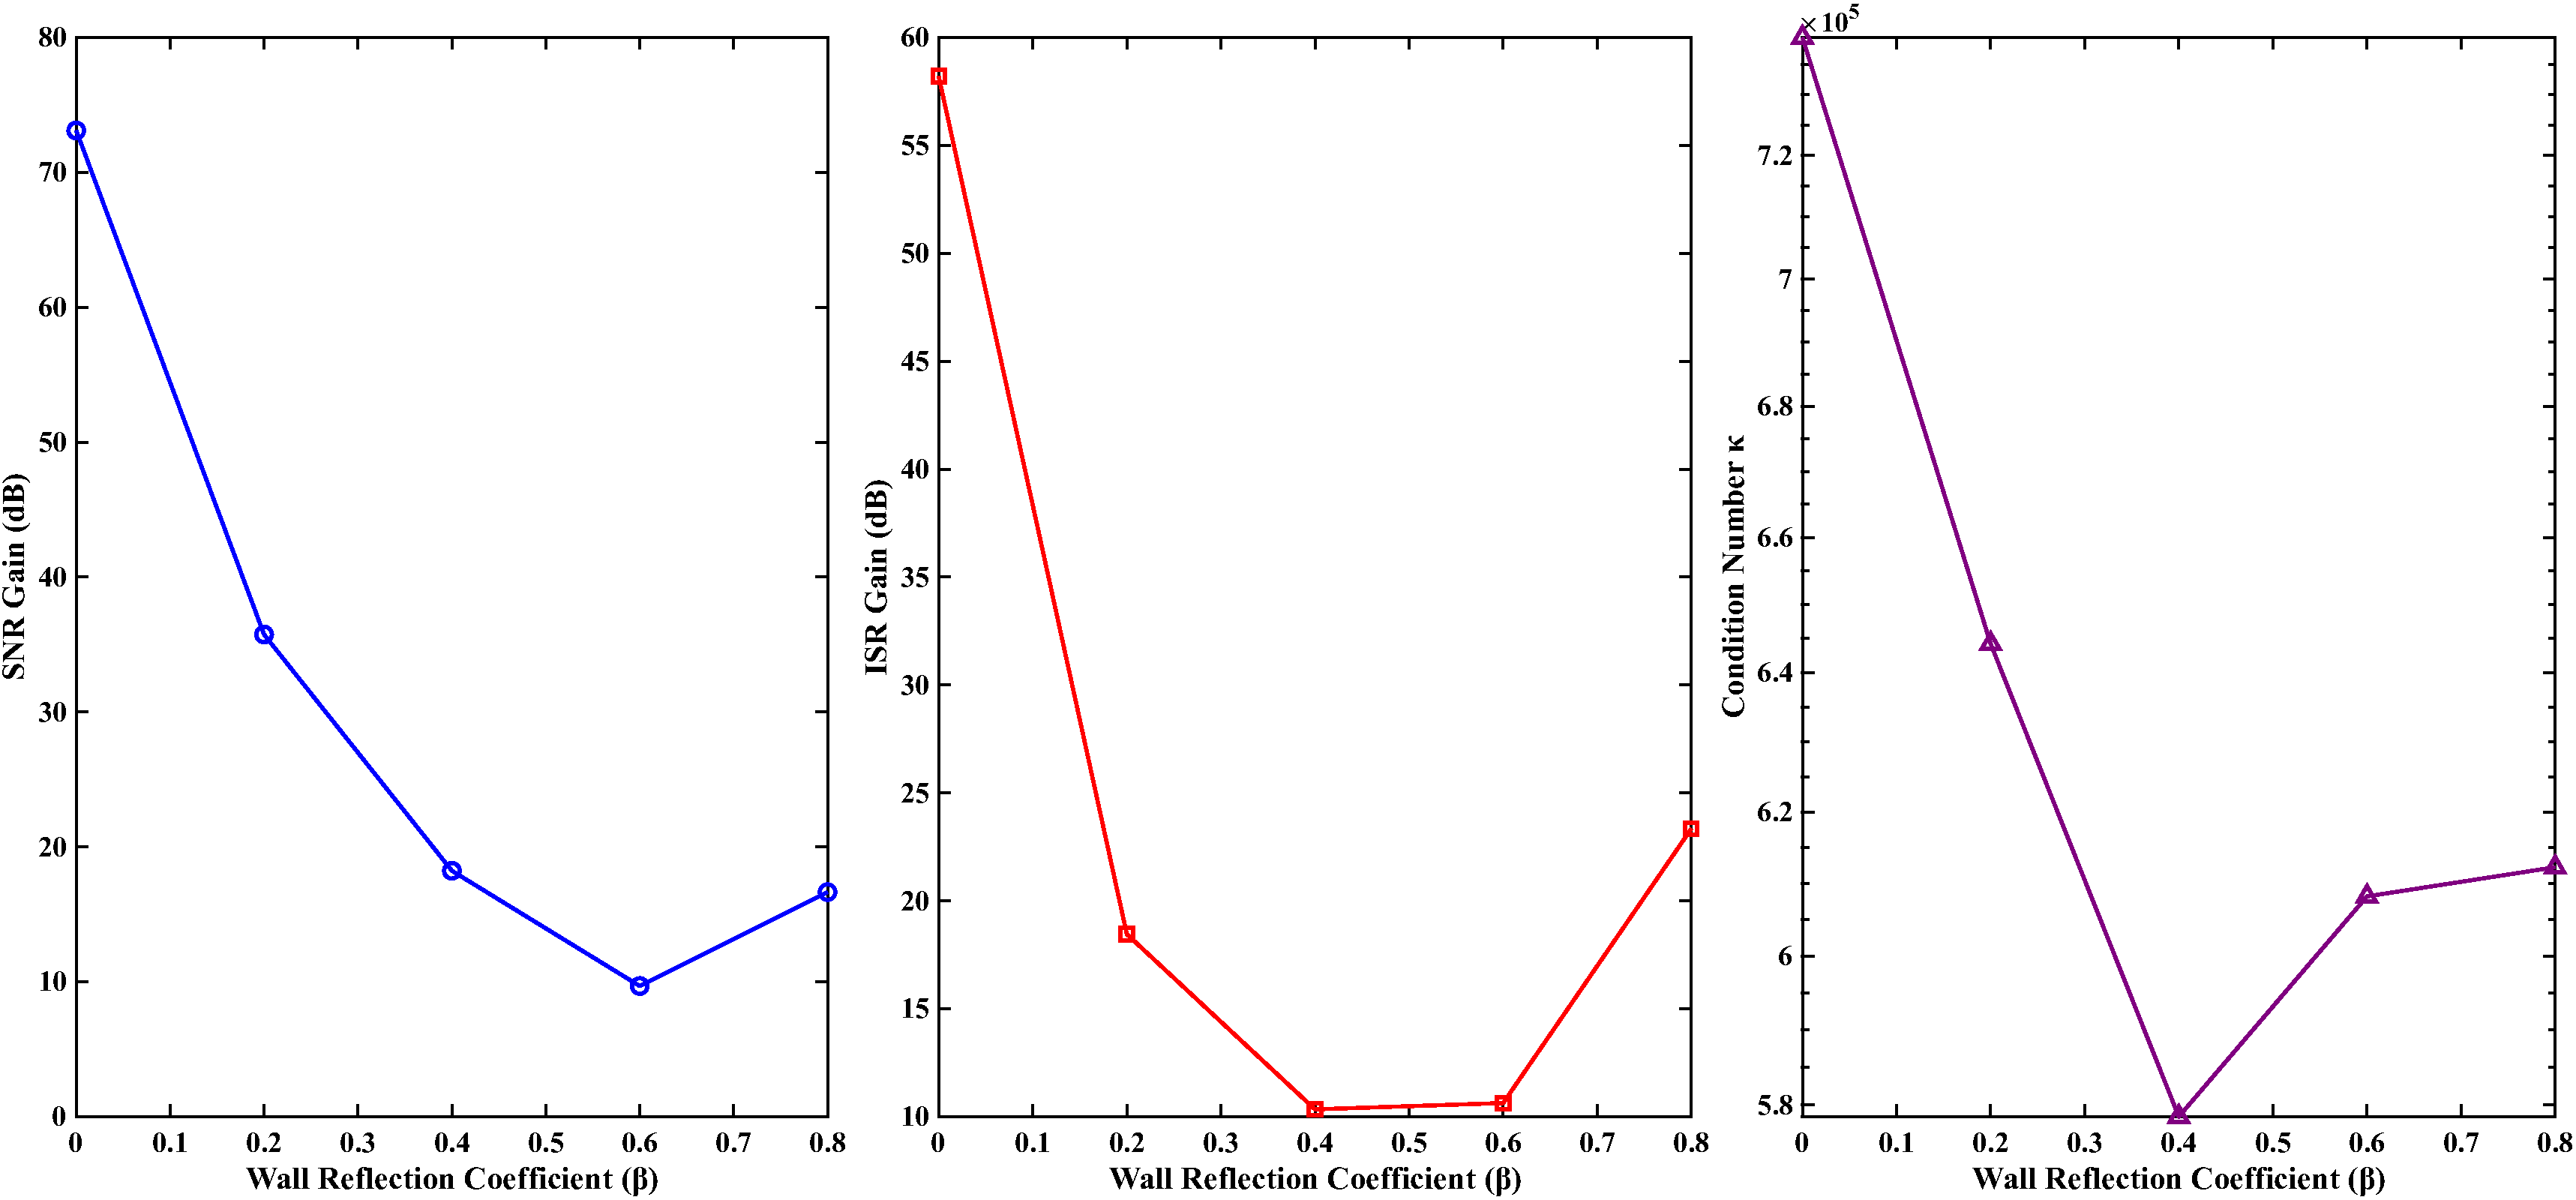
\includegraphics[width=1\linewidth]{output/demo_2k_4k/multi_beta_comparison/Performance_metrics_vs_beta}
\caption{MVDR beamforming performance metrics as functions of wall reflection coefficient $\beta$. (a) SNR improvement for target-steered and interference-steered configurations, showing degradation with increasing reverberation. (b) Beampattern main lobe width (3 dB beamwidth) at 2 kHz, indicating broadening due to multipath effects. (c) Interference suppression level at 4 kHz, demonstrating reduced null depth with increasing $\beta$.}
\label{Performance_metrics_vs_beta}
\end{figure}

\begin{table}[!t]
\centering
\caption{Performance Comparison Under Different $\beta$ Values}
\label{tab:beta_performance}
\renewcommand{\arraystretch}{1.15}
\begin{tabular}{cccc}
\toprule
$\beta$ & SNR Gain (dB) & ISR Gain (dB) & Condition Number ($\kappa$) \\
\midrule
0   & 73.10 & 58.21 & $7.40 \times 10^{5}$ \\
0.2 & 35.74 & 18.46 & $6.44 \times 10^{5}$ \\
0.4 & 18.23 & 10.34 & $5.78 \times 10^{5}$ \\
0.6 & 9.69  & 10.63 & $6.08 \times 10^{5}$ \\
0.8 & 16.64 & 23.35 & $6.12 \times 10^{5}$ \\
\bottomrule
\end{tabular}
\end{table}















% \subsubsection{Beampattern Analysis}

% The beampattern visualization in Fig. \ref{fig:beampattern} clearly shows the main lobe directed towards the target signal and deep nulls in the direction of the interference, demonstrating the spatial filtering capability of the MVDR beamformer in this scenario.
% \begin{figure}
% \centering
% \includegraphics[width=1\linewidth]{demo/Beampattern_2kHz}
% \caption{Beampattern of the MVDR beamformer at 2 kHz. The main lobe is directed towards the target signal, while deep nulls are observed in the direction of the interference, indicating effective spatial filtering.}
% \label{fig:beampattern}
% \end{figure}


% \subsubsection{SINR Performance}

% Using the first microphone channel as the reference, the Signal-to-Interference-plus-Noise Ratio (SINR) improvement is calculated to quantify the enhancement of the target signal relative to the interference and noise. The input SINR is computed based on the power of the target signal and the combined power of interference and noise in the original multichannel signals. The output SINR is calculated similarly for the MVDR beamformed output signal. The difference between the output SINR and input SINR provides a measure of the improvement achieved by the MVDR beamforming process as shown in Table \ref{tab:sinr_improvement}.

% \begin{table}[htbp]
% \centering
% \caption{SINR Improvement of MVDR Beamforming}
% \label{tab:sinr_improvement}
% \begin{tabular}{cc}
% \hline
% \textbf{Metric} & \textbf{Value (dB)} \\
% \hline
% Input SINR & 5 dB \\
% Output SINR & 27.66 dB \\
% SINR Improvement ($\Delta$SINR) & 22.66 dB \\
% \hline
% \end{tabular}
% \end{table}






\subsubsection{Spectrogram comparison}
Fig. \ref{Signal_comparison_spectrograms_input_vs_mvdr} illustrates the MVDR beamforming performance in the time-frequency 
domain. The mixed received signal (left panel) contains equal power target 
(2 kHz) and interference (4 kHz) components. 
The target-steered MVDR branch (center panel) achieves selective 
interference suppression of 42.85 dB at 4 kHz while preserving the target 
signal. Conversely, the interference-steered branch (right panel) provides 
robust target suppression of 60.18 dB at 2 kHz, demonstrating the 
complementary spatial filtering characteristics of the dual-branch 
architecture.

\begin{figure*}
\centering
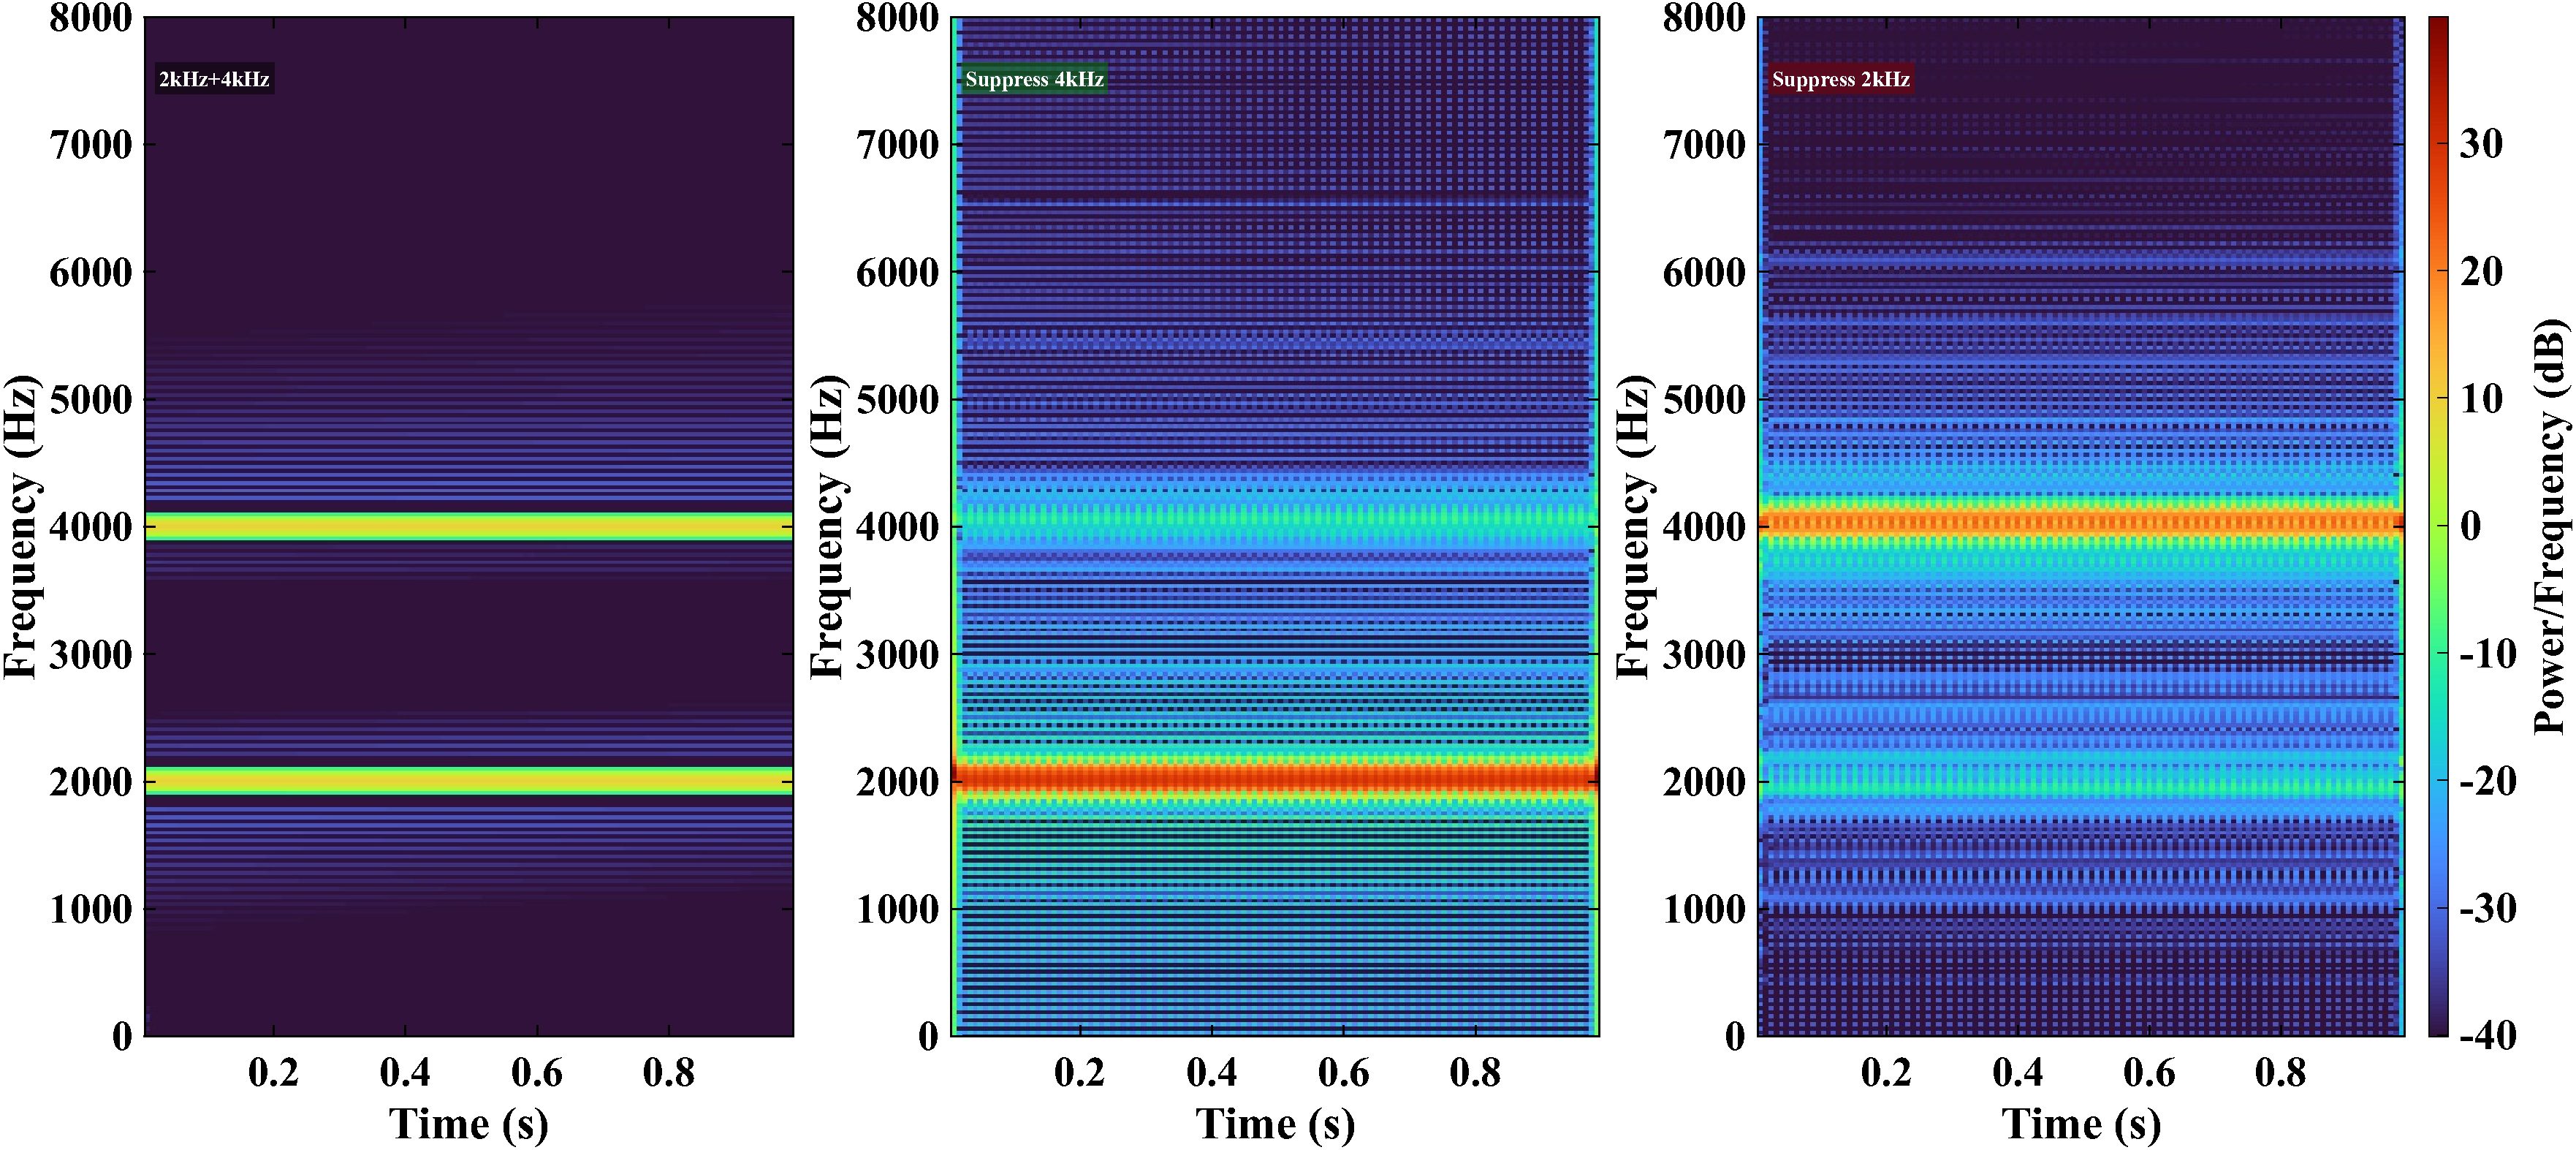
\includegraphics[width=1\linewidth]{output/demo_2k_4k/figures/MVDR_interference_suppression_comparison}
\caption{Time-frequency spectrograms demonstrating MVDR beamforming performance. 
(Left) Input received signal at microphone 1 containing target (2 kHz) 
and interference (4 kHz) components. (Center) Target-steered MVDR output 
showing selective enhancement of the 2 kHz target signal and suppression 
of the 4 kHz interference by 42.85 dB. (Right) Interference-steered MVDR 
output showing suppression of the 2 kHz target by 60.18 dB while 
preserving the 4 kHz interference component.}
\label{Signal_comparison_spectrograms_input_vs_mvdr}
\end{figure*}

\subsubsection{SINR}


\subsection{Simulation 2: Acoustic Signals}
We also conducted a experiment using real acoustic signals recorded from power transformer equipment. The target and interference signal are fault and normal signature captured from transformers, respectively. The Gauss white noise is adopted to simulate real background. Both signals are convolved with their respective RIRs to generate multichannel received signals at the microphone array. The spectral characteristics of the real signals are more complex than the narrowband sinusoids, with the target signal exhibiting multiple frequency components associated with the fault condition. The interference signal has a wideband spectrum, overlapping with the target signal frequencies, as shown in the PSD plot in Fig. \ref{fig:real_signal_configuration}. This scenario provides a realistic test case for evaluating the MVDR beamforming performance in enhancing the target fault signature while suppressing broadband interference in a practical acoustic environment.
\begin{figure}
\centering
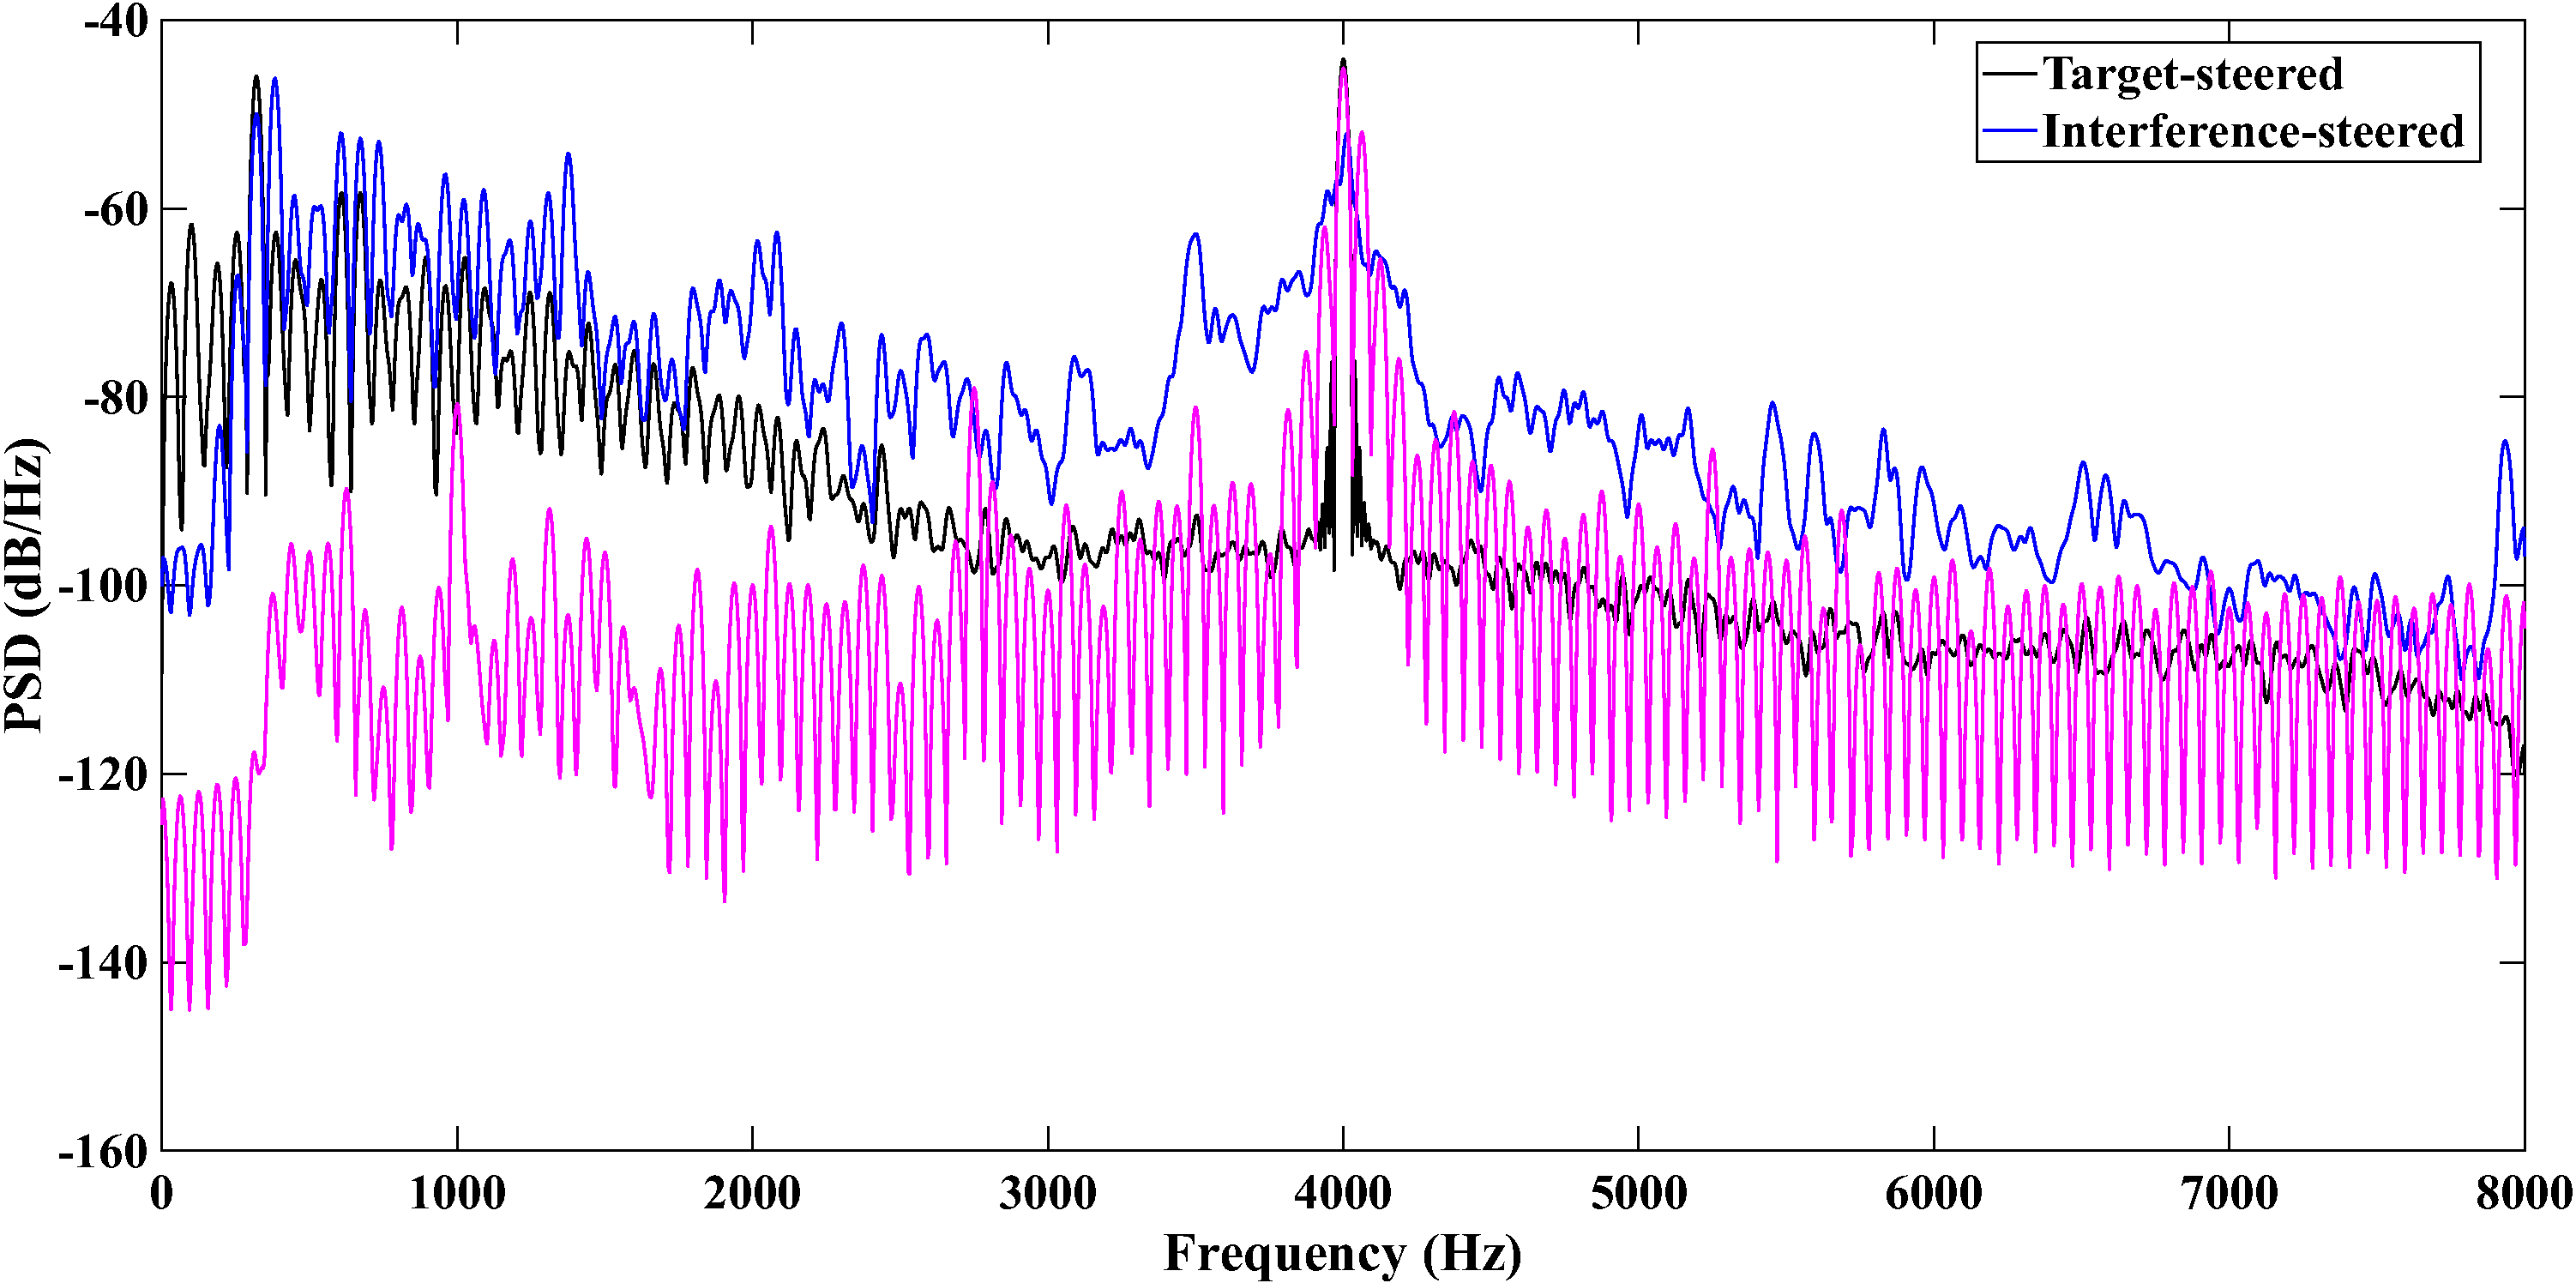
\includegraphics[width=1\linewidth]{output/real_signal/figures/PSD_fullband}
\caption{Power Spectral Density (PSD) of the real target and interference signals after RIR convolution. The target signal exhibits multiple frequency components, while the interference signal has a wideband spectrum overlapping with the target frequencies.}
\label{fig:real_signal_configuration}
\end{figure}


After applying the MVDR beamforming algorithm to the received multichannel signals, the output signal is analyzed in terms of its spectral content and spatial characteristics. The comparison between the input and output signals in the frequency domain reveals the effectiveness of the MVDR beamformer in suppressing the interference while preserving the target signal. As shown in Fig. \ref{Signal_comparison_spectrograms_input_vs_mvdr}, the spectrograms of the input and output signals show a significant reduction in the interference components while maintaining the integrity of the target signal. 

\begin{figure*}
\centering
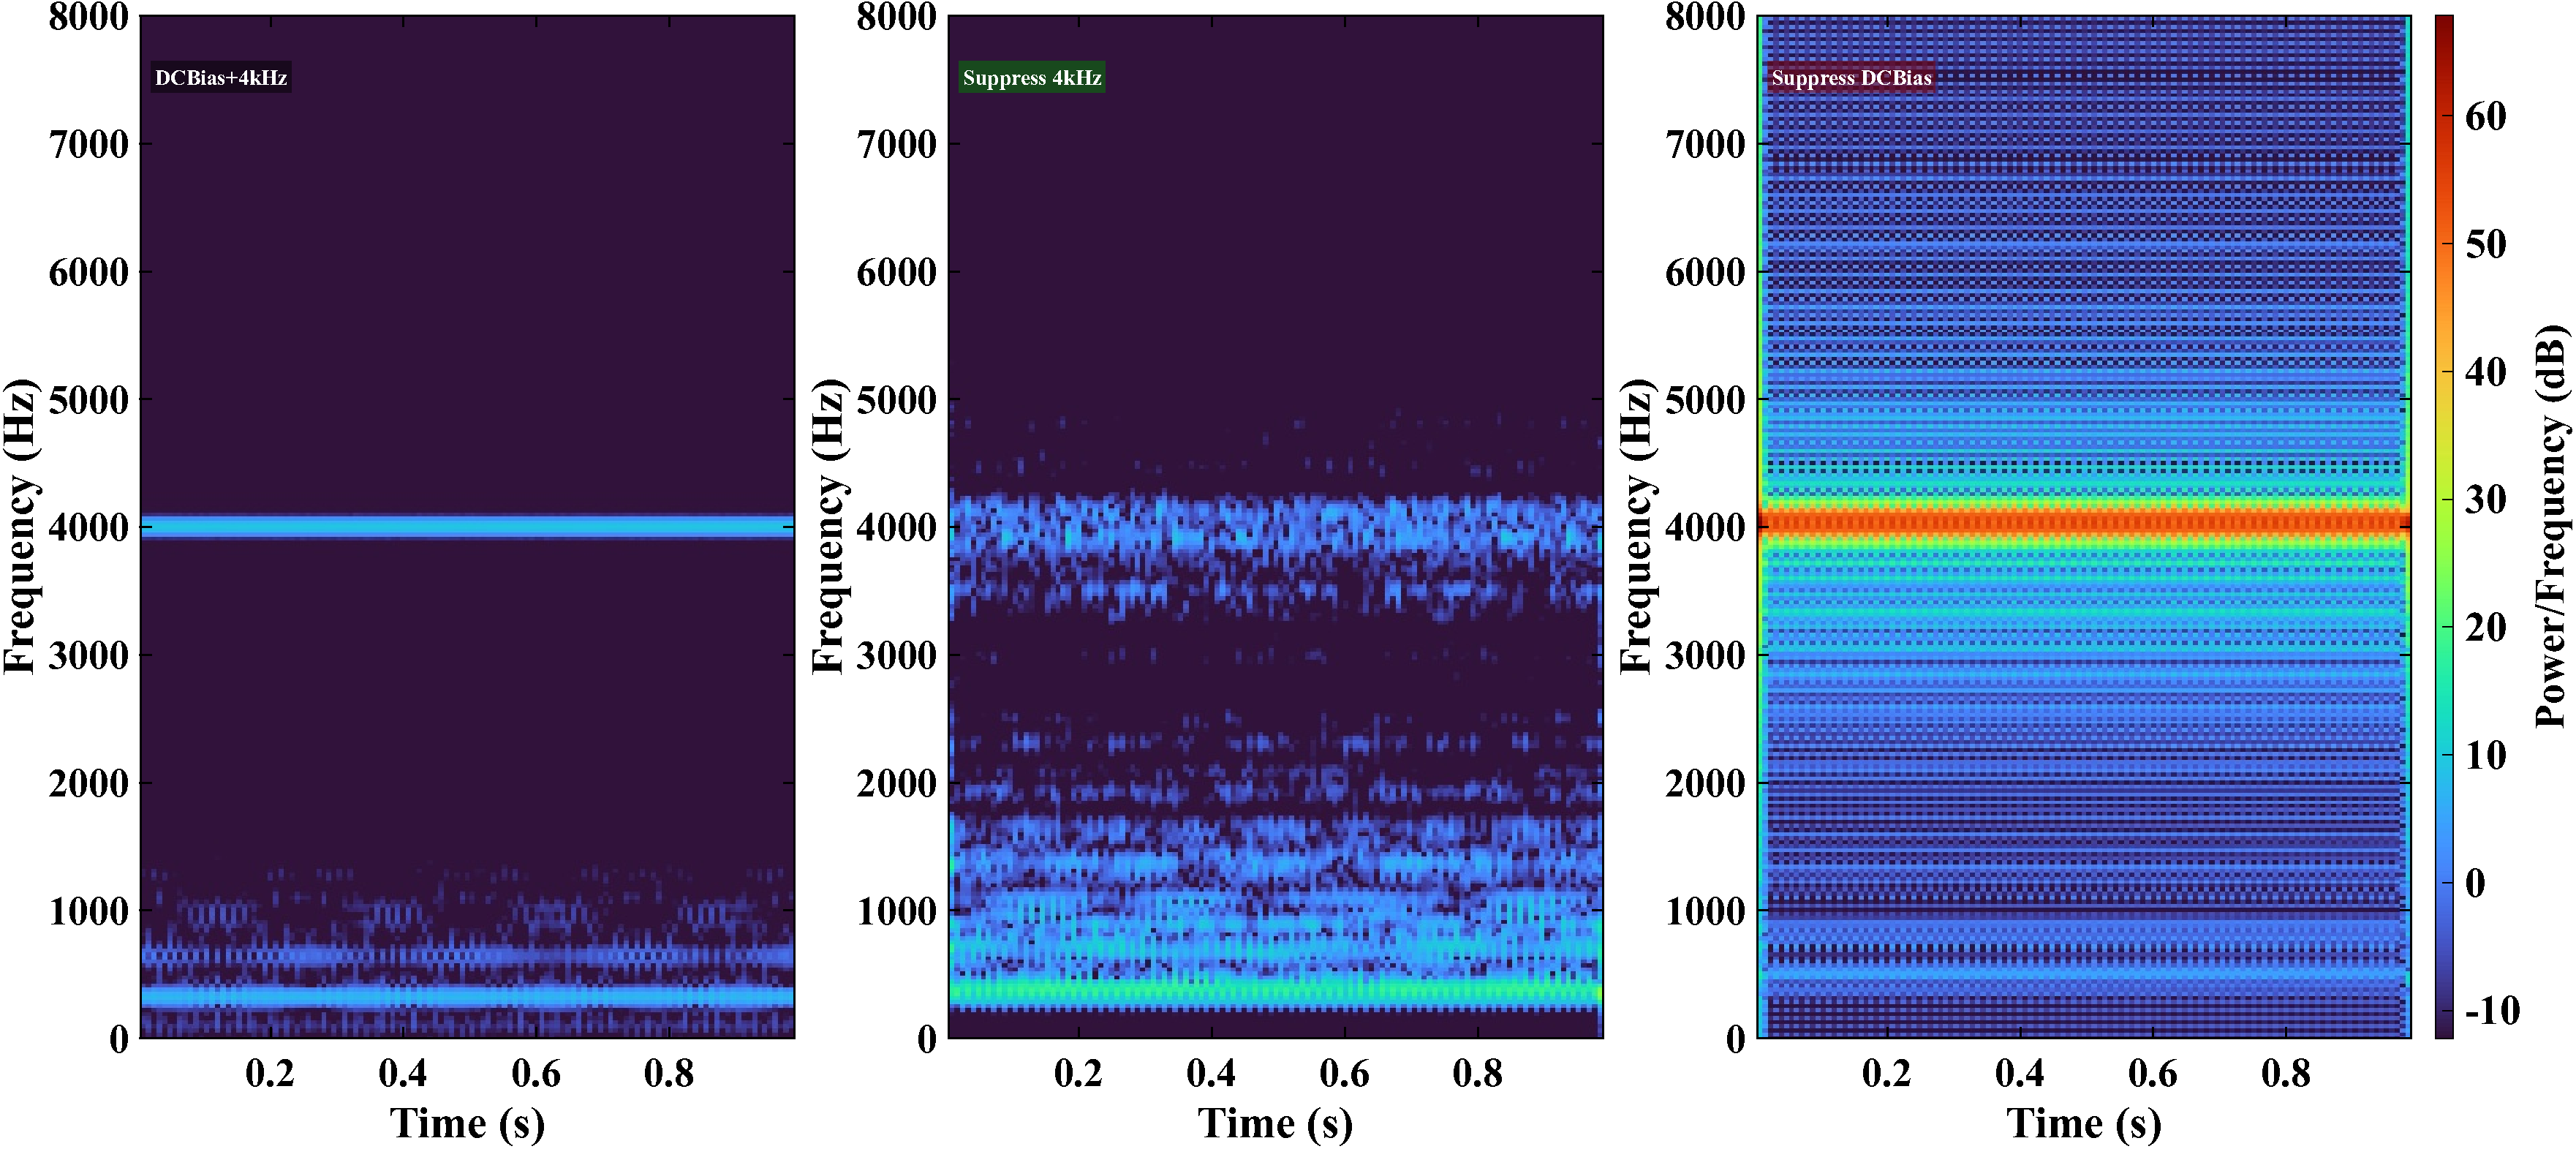
\includegraphics[width=1\linewidth]{output/real_signal/figures/MVDR_interference_suppression_comparison}
\caption{Spectrogram comparison between the input signal and the MVDR beamformed output signal. The MVDR output shows significant suppression of interference components while preserving the target signal.}
\label{Signal_comparison_spectrograms_input_vs_mvdr}
\end{figure*}



\begin{figure}
\centering
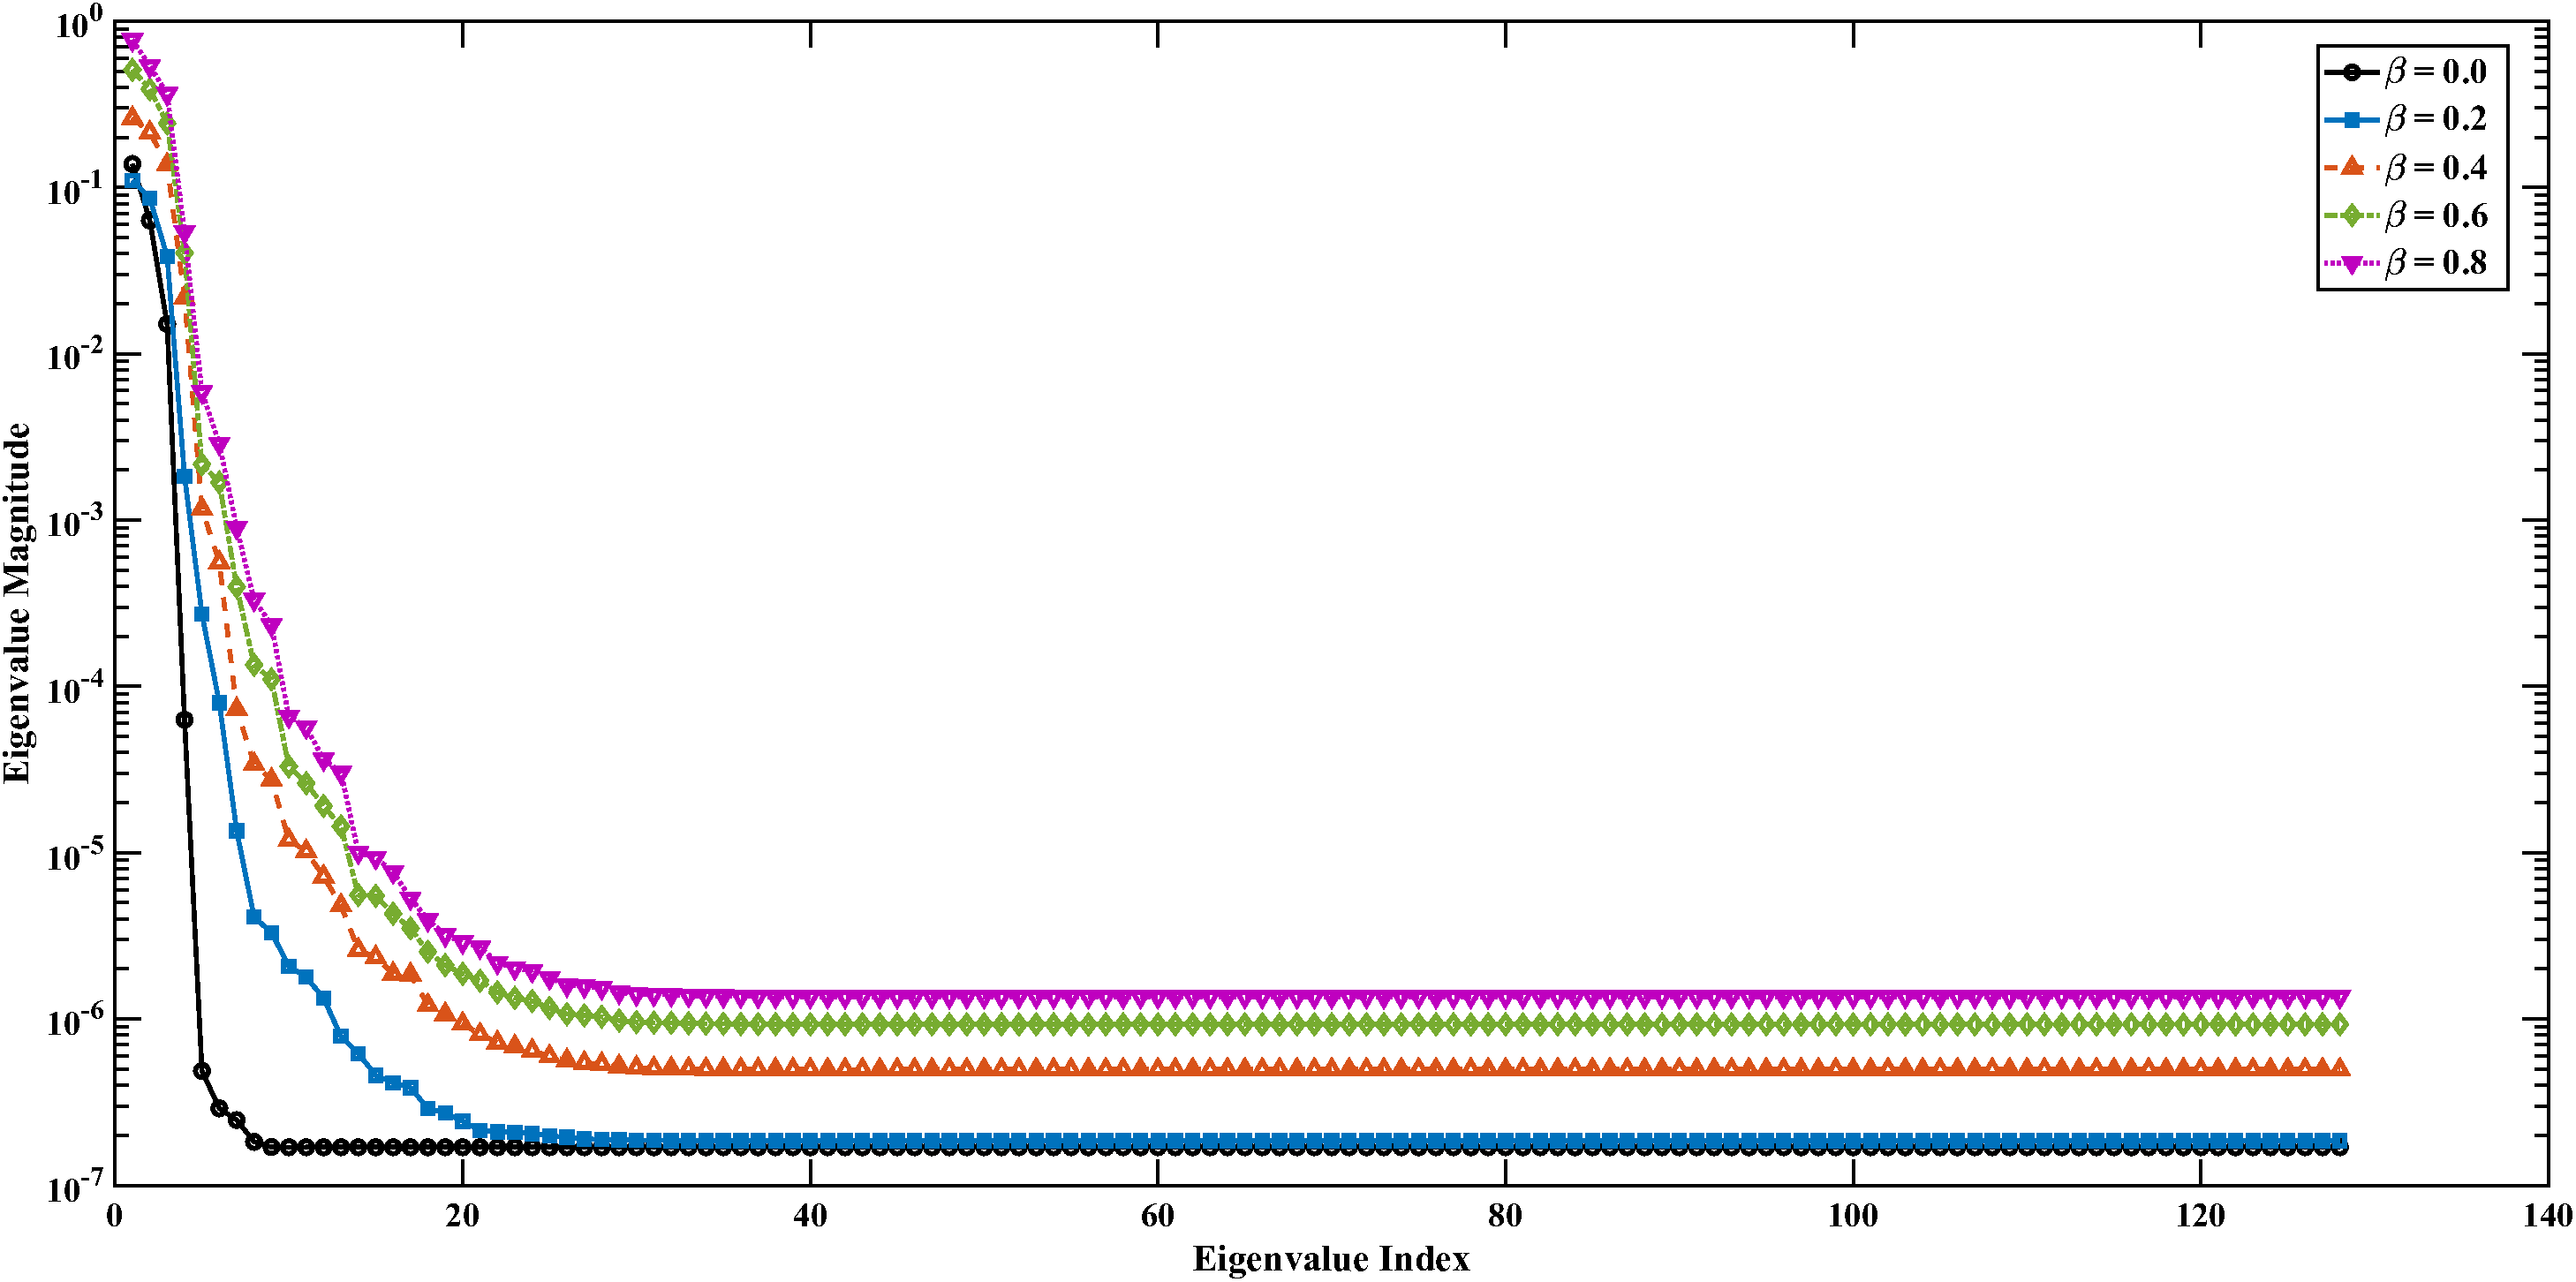
\includegraphics[width=1\linewidth]{output/real_signal/multi_beta_comparison/Eigenspectra_fullband_comparison}
\caption{}
\label{} 
\end{figure}



The beampattern is shown in Fig. \ref{fig:beampattern}. The epsilon value for diagonal loading is set to $10^{-4}$, which provides sufficient regularization to ensure numerical stability of the covariance matrix inversion while preserving the adaptive suppression capability of the MVDR beamformer. This value is determined empirically based on the condition number of the covariance matrix and the observed performance in terms of interference suppression and target signal preservation. The comparison ofbeamformer performance is shown in Table \ref{tab:beamformer_performance}.


\begin{table*}[htbp]
\centering
\caption{Beamformer performance summary for different $\epsilon$ settings}
\label{tab:beamformer_performance}
\begin{tabular}{cccccccc}
\toprule
\textbf{Mavg} & \textbf{$\epsilon$} & \textbf{shrink\_alpha} & \textbf{$BW_{-3\mathrm{dB}}$ (deg)} & \textbf{Main Lobe} & \textbf{Side Lobes} & \textbf{Side Lobes ratio} & \textbf{azimuth (deg)} \\
\midrule
31 & $1\times10^{-3}$ & 0 & 59.00 & 8.59  & 0.57  & 8.02  & -91.00 \\
31 & $1\times10^{-4}$ & 0 & 52.00 & 11.61 & -3.10 & 10.71 & -7.00 \\
31 & $1\times10^{-5}$ & 0 & 46.00 & 15.80 & 6.40  & 9.40  & -91.00 \\
31 & $1\times10^{-6}$ & 0 & 59.00 & 18.42 & 18.38 & 0.04  & -7.00 \\
\bottomrule
\end{tabular}
\end{table*}


\begin{figure}
\centering
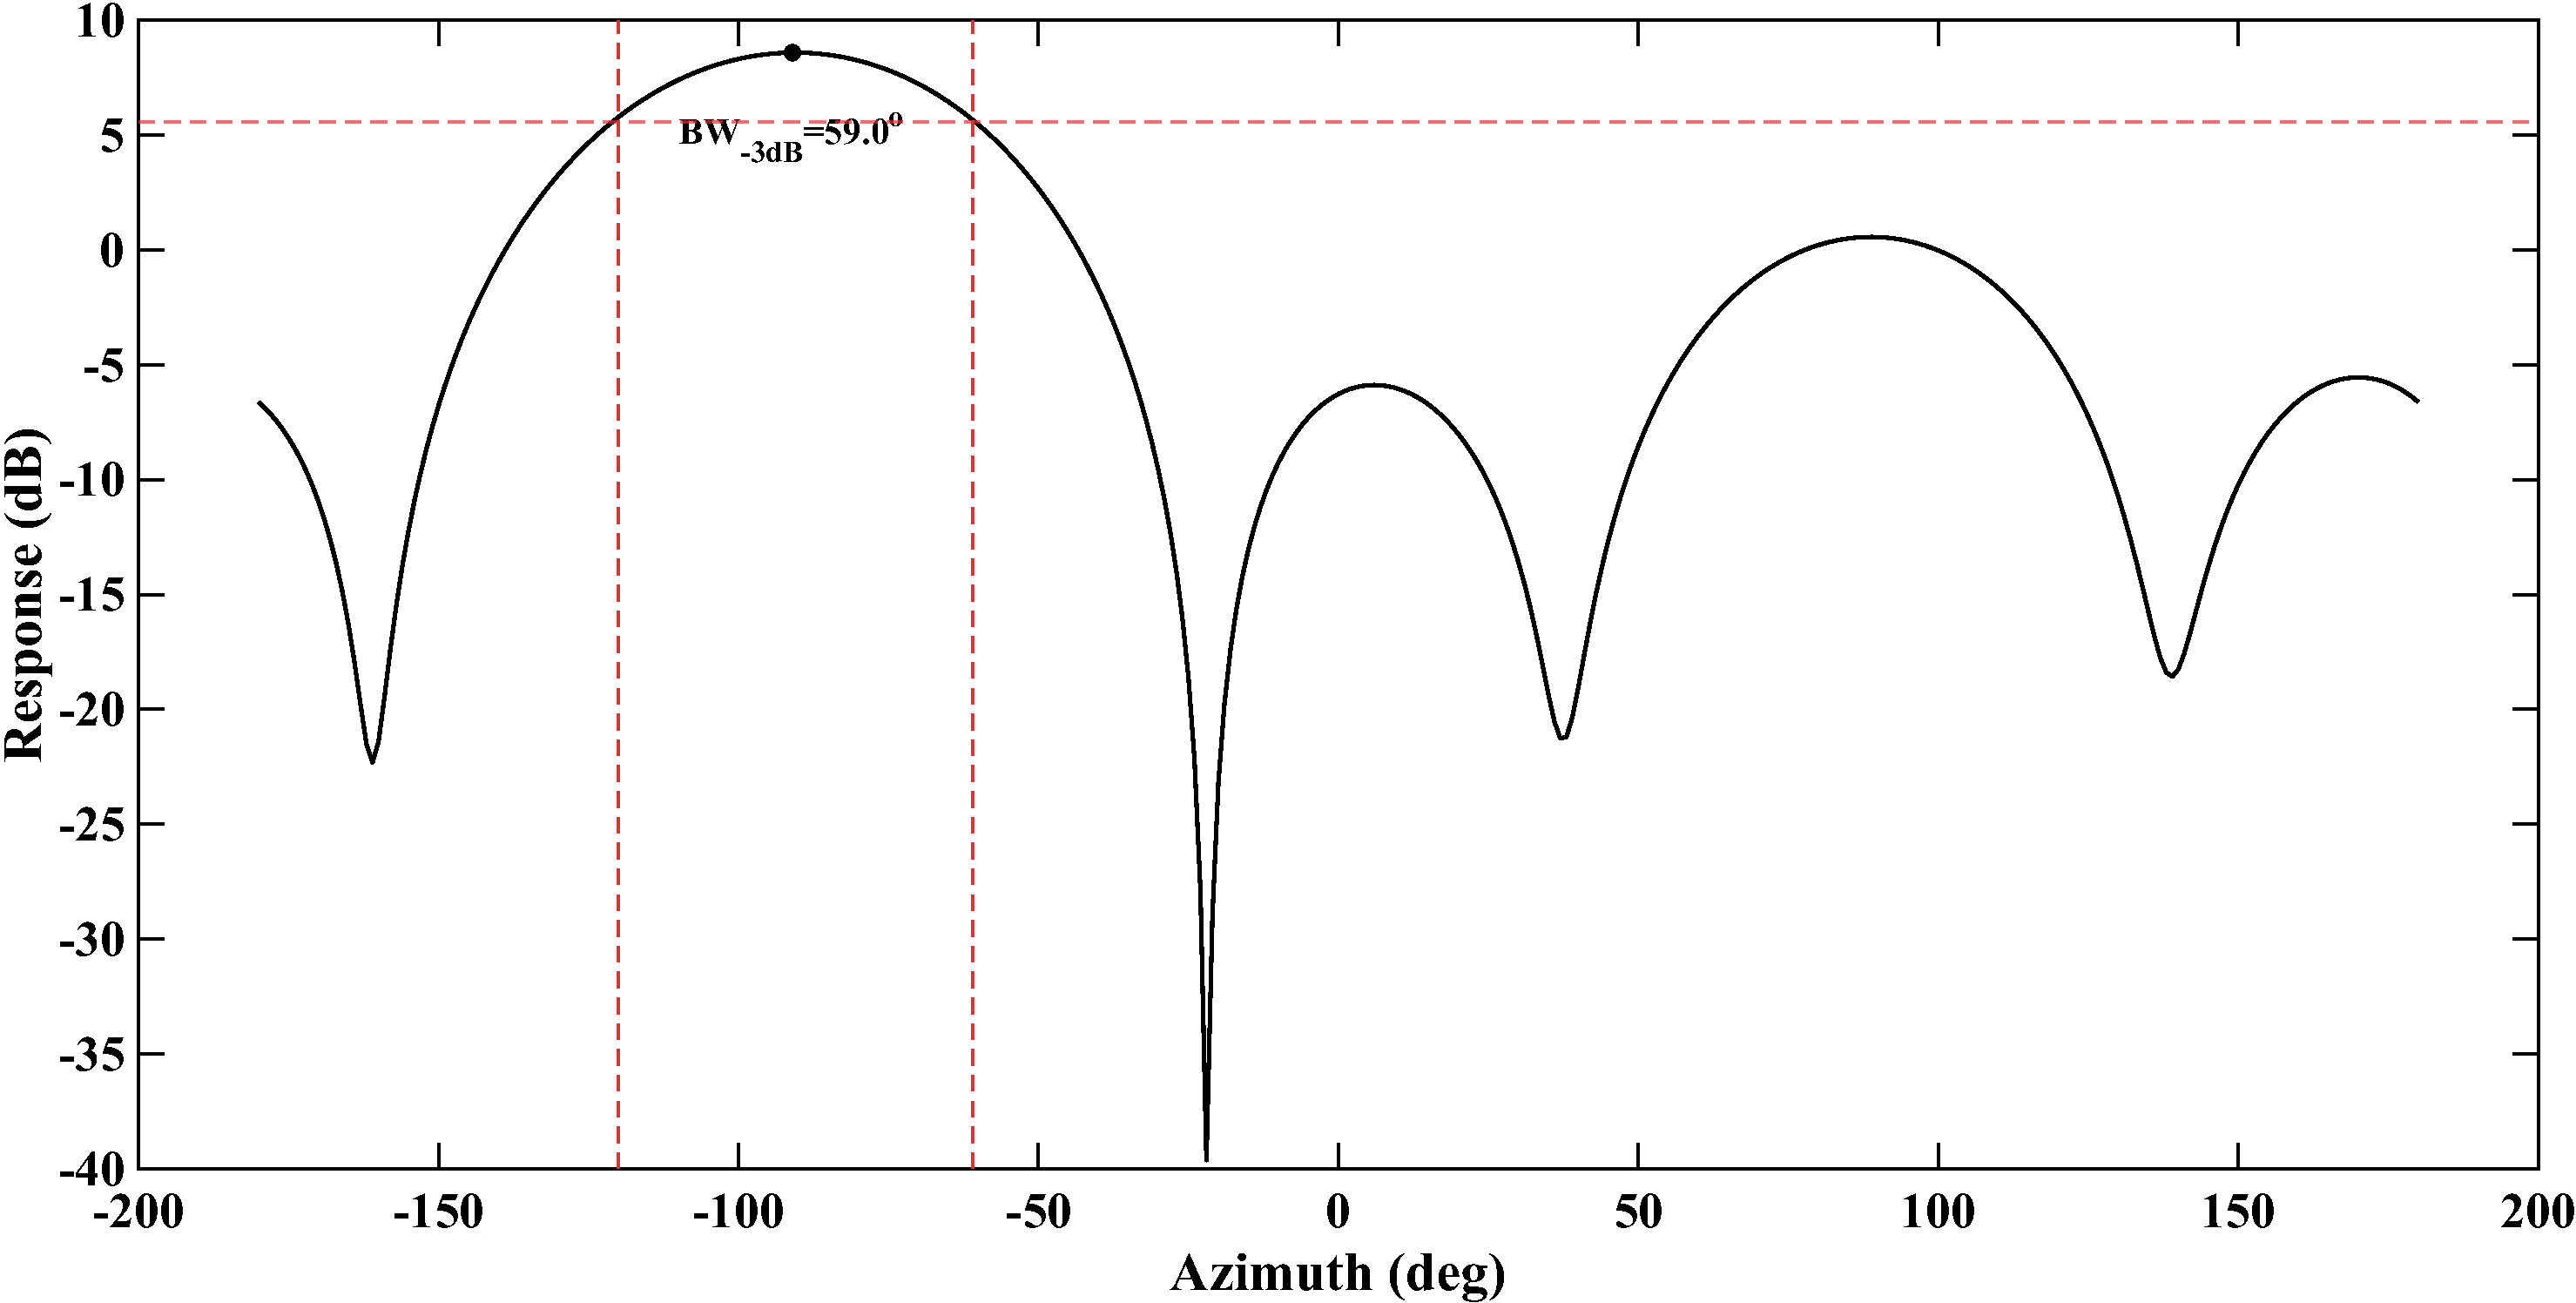
\includegraphics[width=1\linewidth]{output/real_signal/figures/Beampattern}
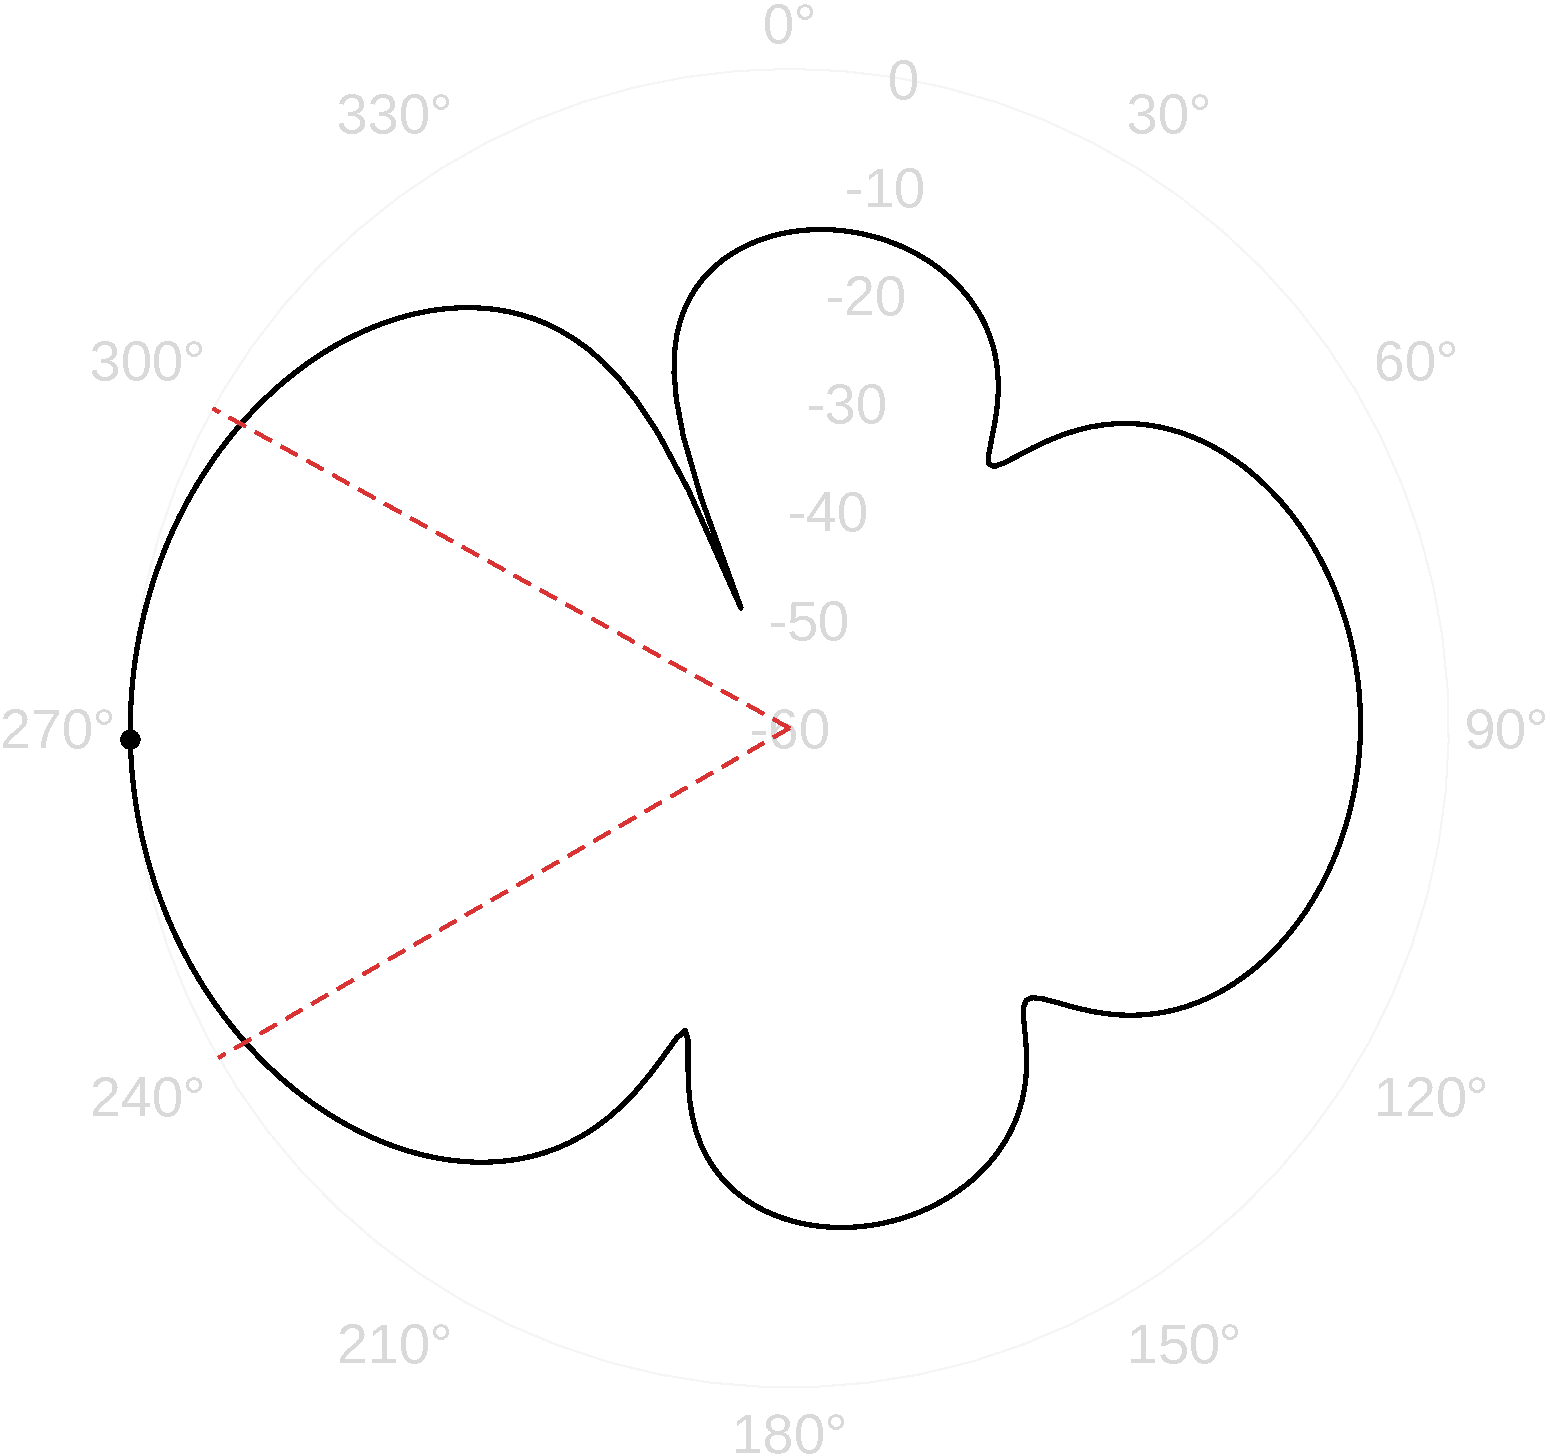
\includegraphics[width=1\linewidth]{output/real_signal/figures/Beampattern_polar}
\caption{Beampattern of the MVDR beamformer at 2 kHz. The main lobe is directed towards the target signal, while deep nulls are observed in the direction of the interference, indicating effective spatial filtering.}
\label{fig:beampattern}
\end{figure}


\subsection{Fault Diagnosis and Performance Metrics}



\subsubsection{Ablation Experiment}

\subsubsection{Comparison Experiment}

To establish a comprehensive benchmark, we evaluate several classical machine learning and deep learning models on the MVDR-enhanced spectrogram dataset. Table~\ref{tab:model_comparison} summarizes the classification performance and computational complexity of each model.

\begin{table*}[htbp]
\centering
\caption{Model Performance Comparison on MVDR-Enhanced Spectrogram Dataset}
\label{tab:model_comparison}
\renewcommand{\arraystretch}{1.15}
\begin{tabular}{lcccccc}
\toprule
\textbf{Model} & \textbf{Accuracy} & \textbf{Precision} & \textbf{Recall} & \textbf{F1} & \textbf{Train Time (s)} & \textbf{Trainable Params} \\
\midrule
SVM (RBF)      & 1.000 & 1.000 & 1.000 & 1.000 & 2.48  & 4,104 \\
Random Forest  & 1.000 & 1.000 & 1.000 & 1.000 & 15.71 & 9,652 \\
LDA            & 1.000 & 1.000 & 1.000 & 1.000 & 0.04  & 118 \\
MLP (Small)    & 1.000 & 1.000 & 1.000 & 1.000 & 3.87  & 4,900 \\
Transfer Learning (ResNet18) & 1.000 & 1.000 & 1.000 & 1.000 & 14.45 & 8,529,220 \\
EfficientNet-B0 (3-Phase)    & 1.000 & 1.000 & 1.000 & 1.000 & 10.81 & 3,485,056 \\
\bottomrule
\end{tabular}
\end{table*}

All models achieve perfect classification on the test set. Table~\ref{tab:confusion_matrix} presents the aggregated confusion matrix, which is identical across all evaluated models. The dataset comprises four fault classes: DCBias (13 samples), Harmonic (13 samples), Loosen (14 samples), and PartialDischarge (14 samples), totaling 54 test samples. Table~\ref{tab:per_class_metrics} reports the per-class precision, recall, and F1-score. The hyperparameter configurations obtained via grid search for each model are summarized in Table~\ref{tab:hyperparameters}.

\begin{table}[htbp]
\centering
\caption{Per-Class Classification Metrics (Identical for All Models)}
\label{tab:per_class_metrics}
\renewcommand{\arraystretch}{1.15}
\begin{tabular}{lcccc}
\toprule
\textbf{Fault Class} & \textbf{Precision} & \textbf{Recall} & \textbf{F1-Score} & \textbf{Support} \\
\midrule
DCBias            & 1.00 & 1.00 & 1.00 & 13 \\
Harmonic          & 1.00 & 1.00 & 1.00 & 13 \\
Loosen            & 1.00 & 1.00 & 1.00 & 14 \\
PartialDischarge  & 1.00 & 1.00 & 1.00 & 14 \\
\midrule
Macro Avg         & 1.00 & 1.00 & 1.00 & 54 \\
Weighted Avg      & 1.00 & 1.00 & 1.00 & 54 \\
\bottomrule
\end{tabular}
\end{table}

\begin{table*}[htbp]
\centering
\caption{Optimal Hyperparameter Configurations}
\label{tab:hyperparameters}
\renewcommand{\arraystretch}{1.2}
\begin{tabular}{ll}
\toprule
\textbf{Model} & \textbf{Best Hyperparameters} \\
\midrule
SVM (RBF)      & $C=100$, $\gamma=\text{scale}$, kernel=RBF \\
Random Forest  & $n\_\text{estimators}=100$, $\text{max\_depth}=\text{None}$, $\text{max\_features}=\log_2$, \\
               & $\text{min\_samples\_leaf}=1$, $\text{min\_samples\_split}=2$ \\
LDA            & $\text{shrinkage}=\text{None}$ \\
MLP (Small)    & $\text{hidden\_dims}=(64, 32)$, $\text{dropout}=0.3$, $\text{lr}=0.001$, \\
               & $\text{weight\_decay}=0.001$ \\
\bottomrule
\end{tabular}
\end{table*}

\begin{figure*}
\centering
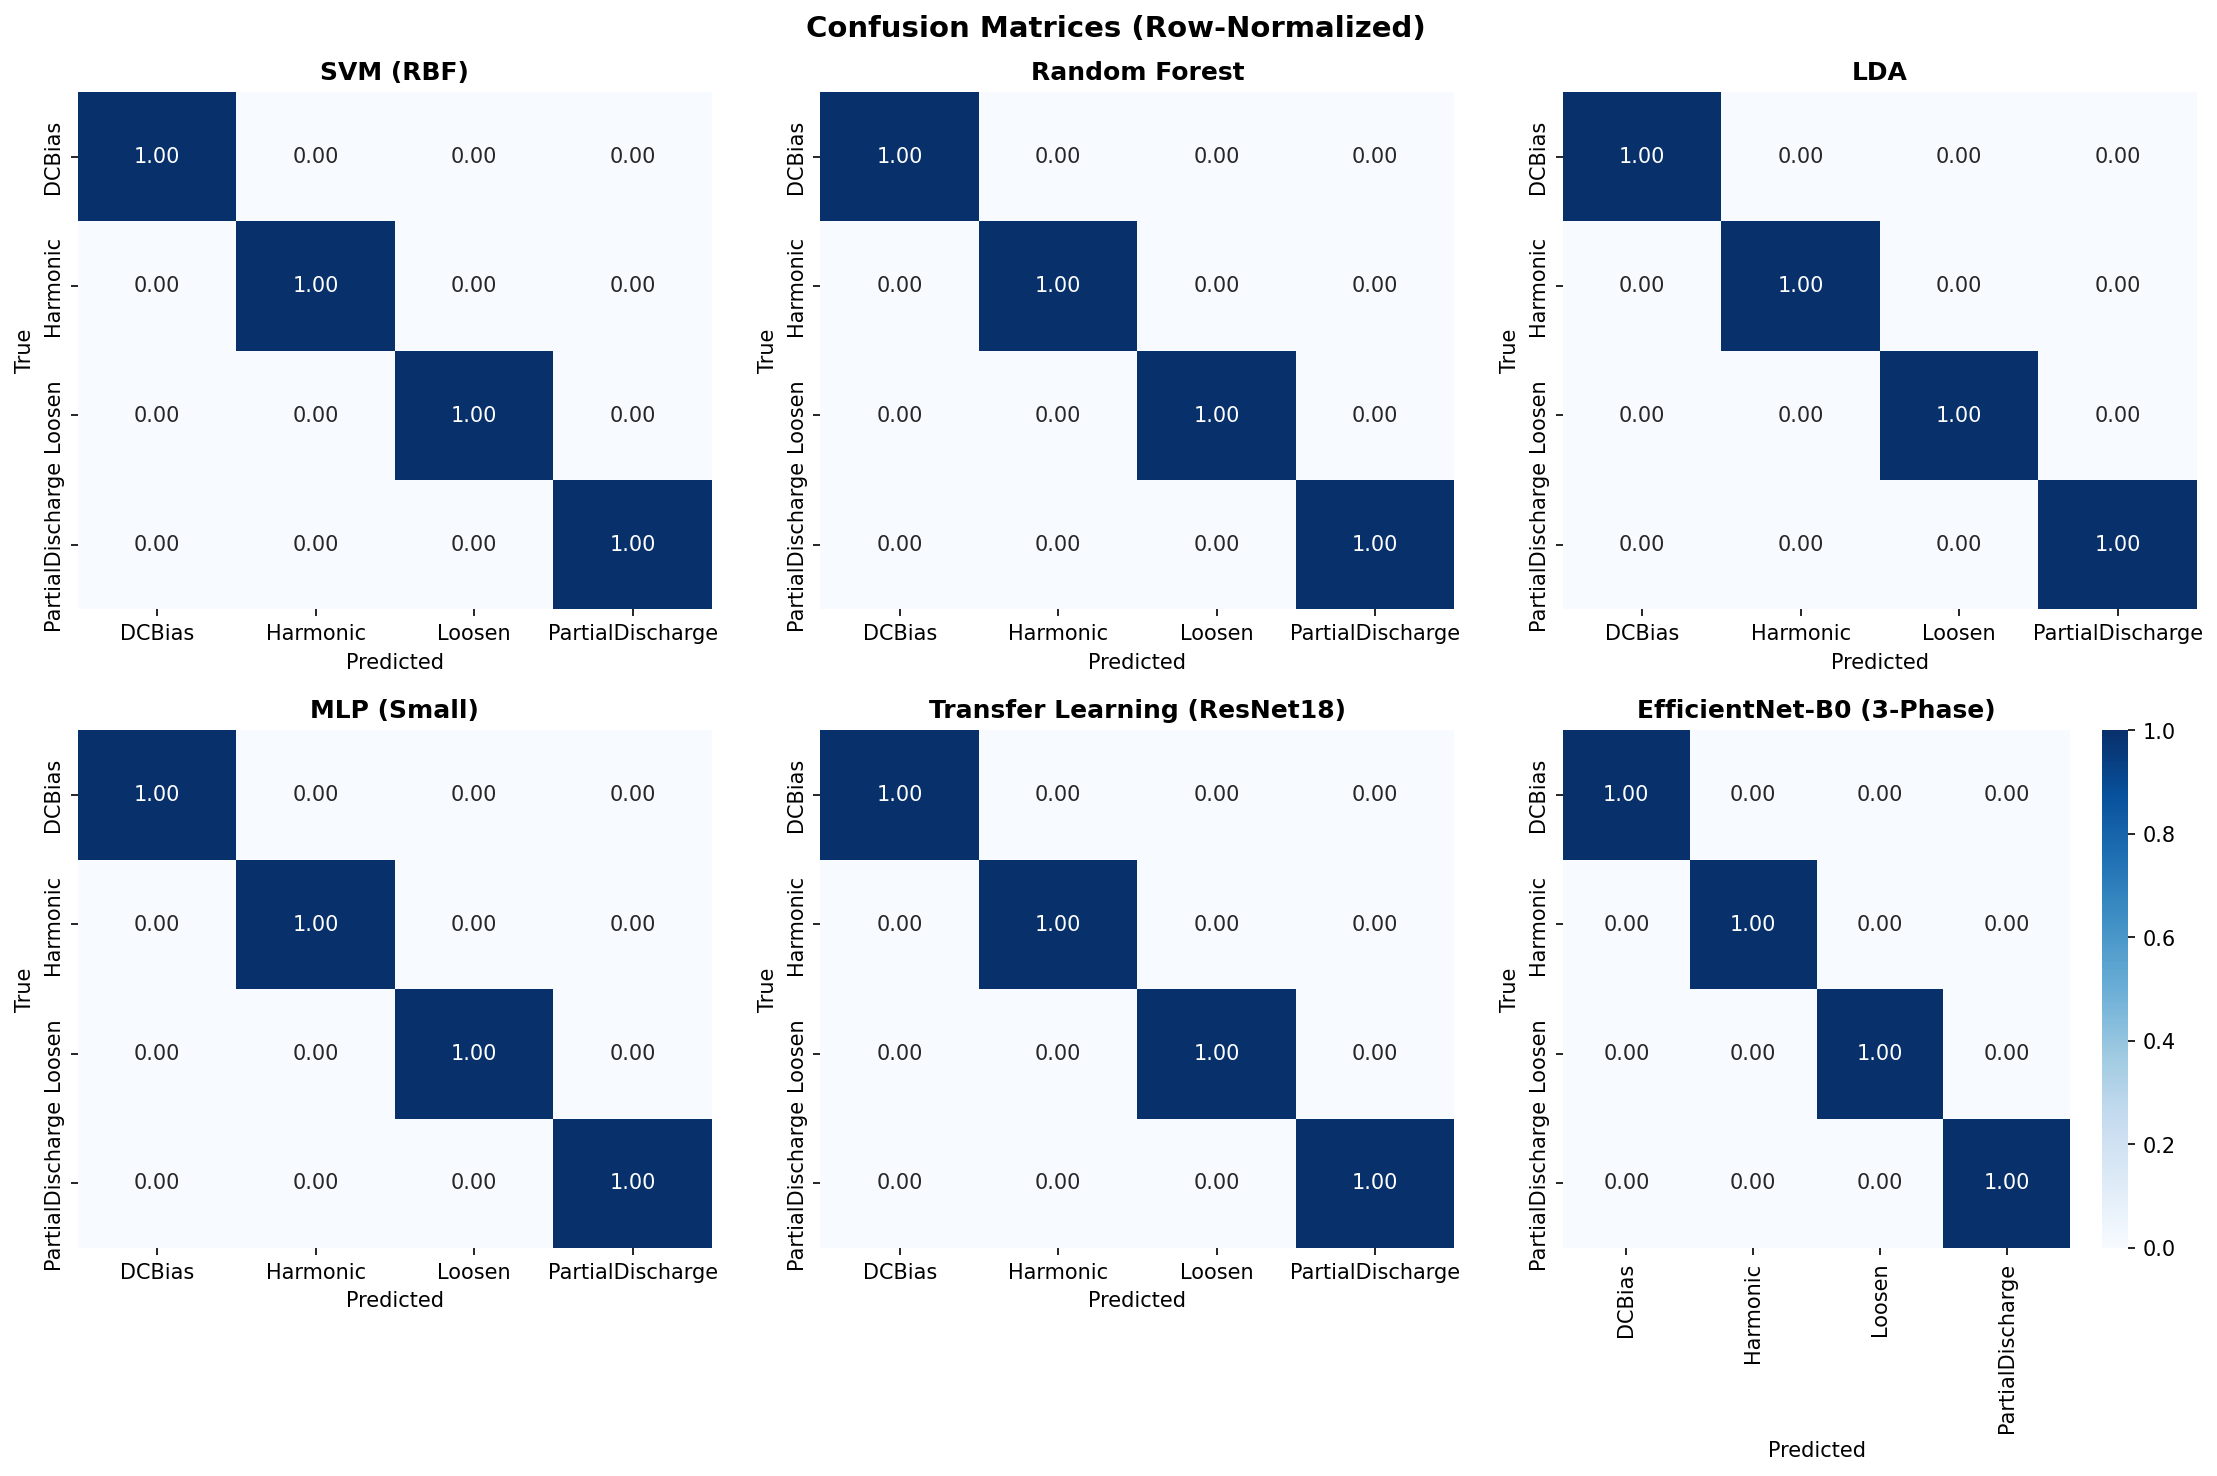
\includegraphics[width=1\linewidth]{results/confusion_matrices}
\caption{}
\label{}
\end{figure*}

\begin{figure*}
\centering
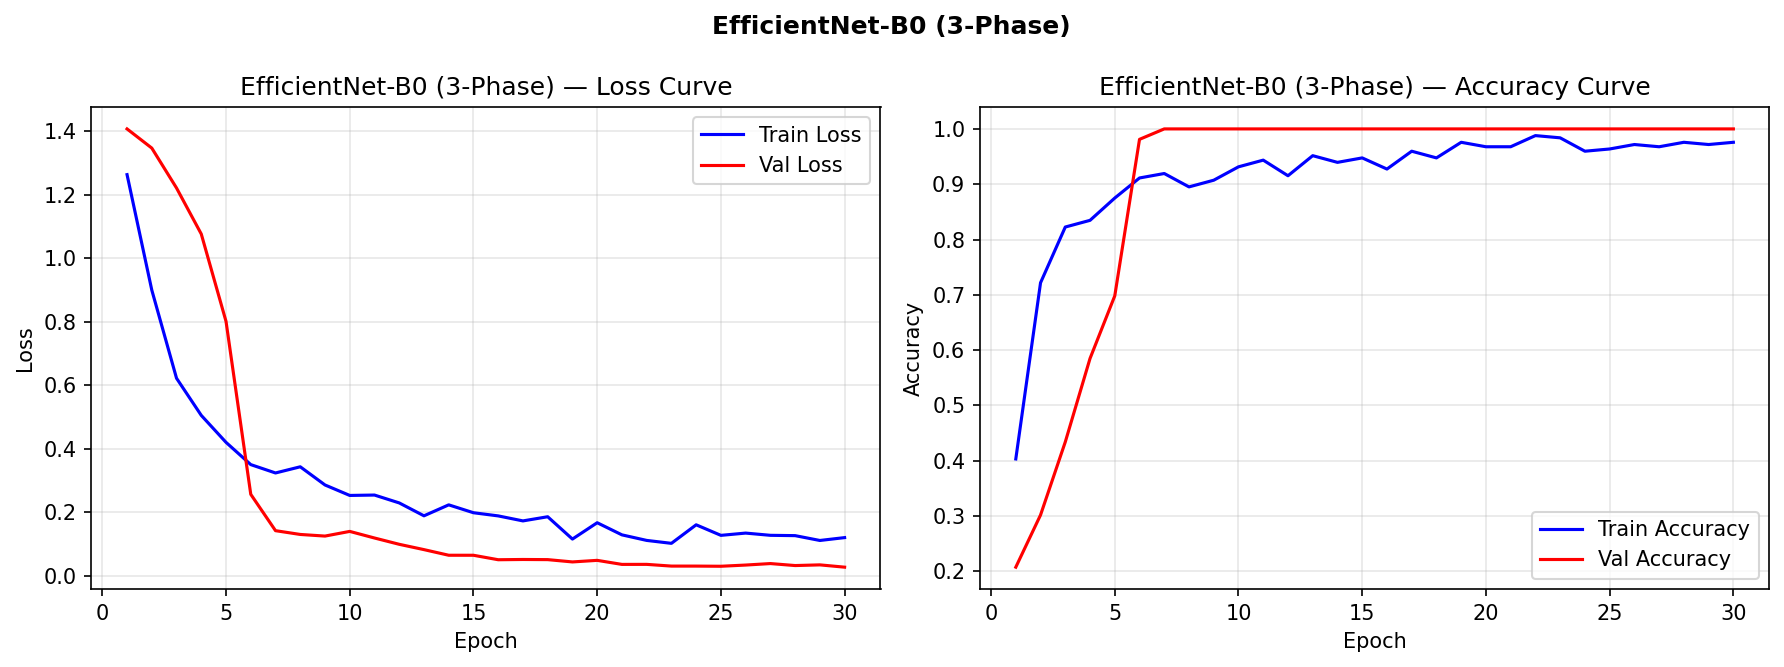
\includegraphics[width=1\linewidth]{results/efficientnet_b0_loss_accuracy}
\caption{}
\label{}
\end{figure*}

\begin{figure*}
\centering
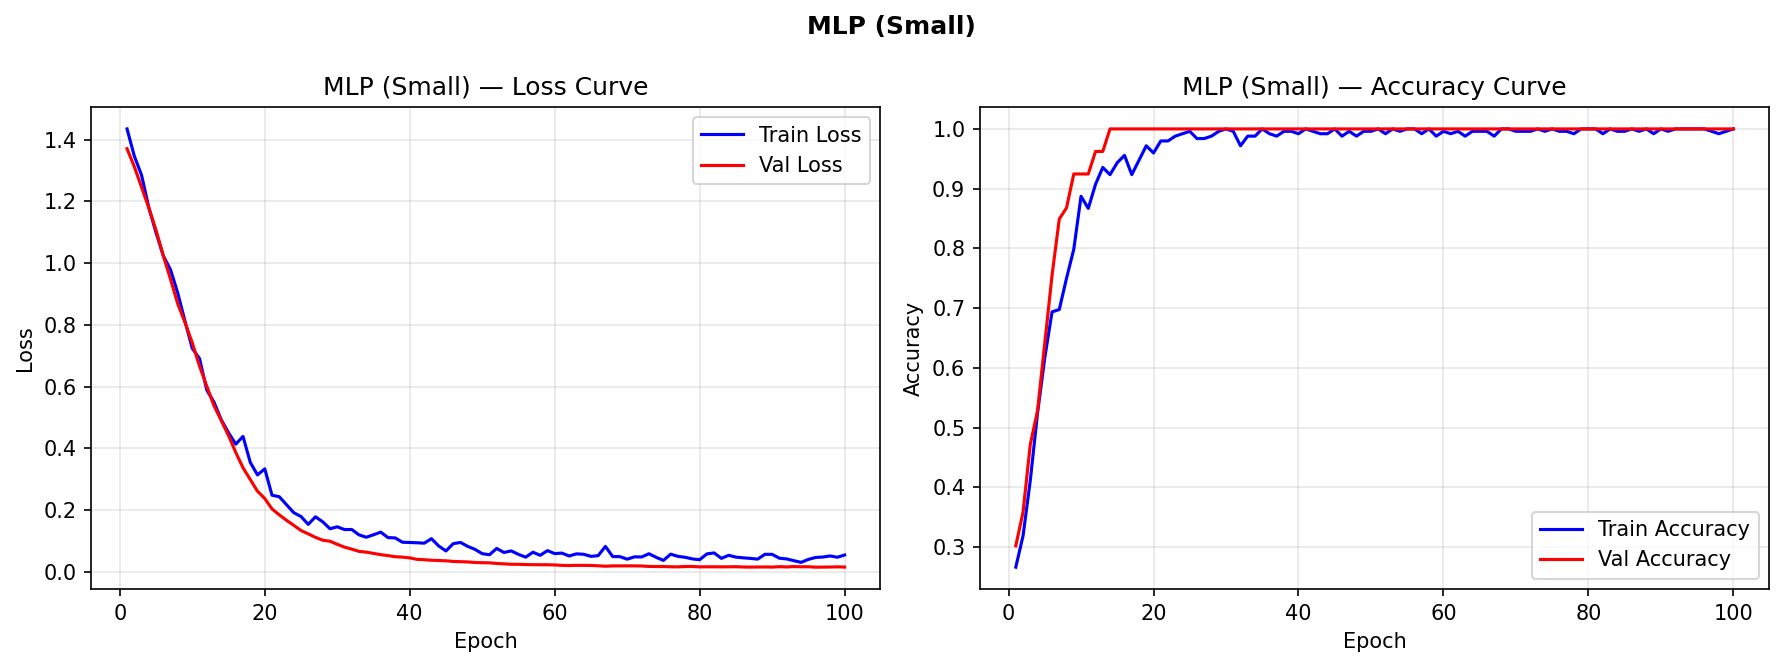
\includegraphics[width=1\linewidth]{results/mlp_loss_accuracy.png}
\caption{}
\label{}
\end{figure*}

\begin{figure*}
\centering
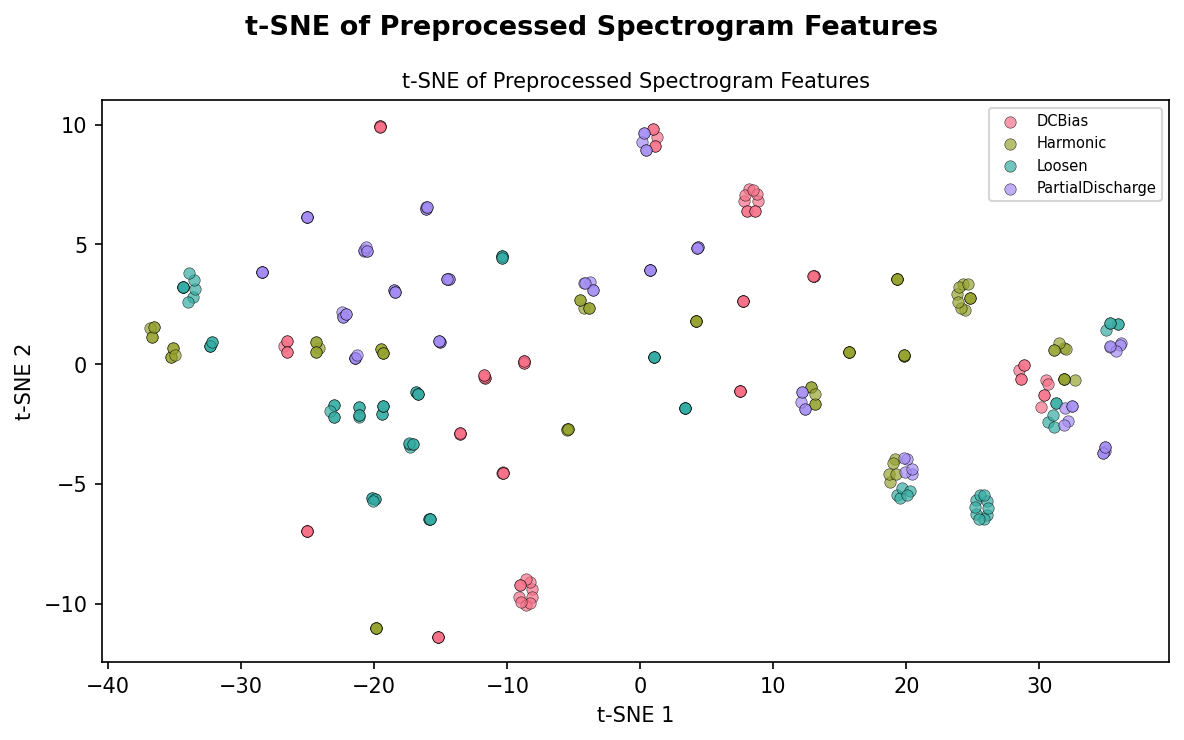
\includegraphics[width=1\linewidth]{results/tsne_embedding}
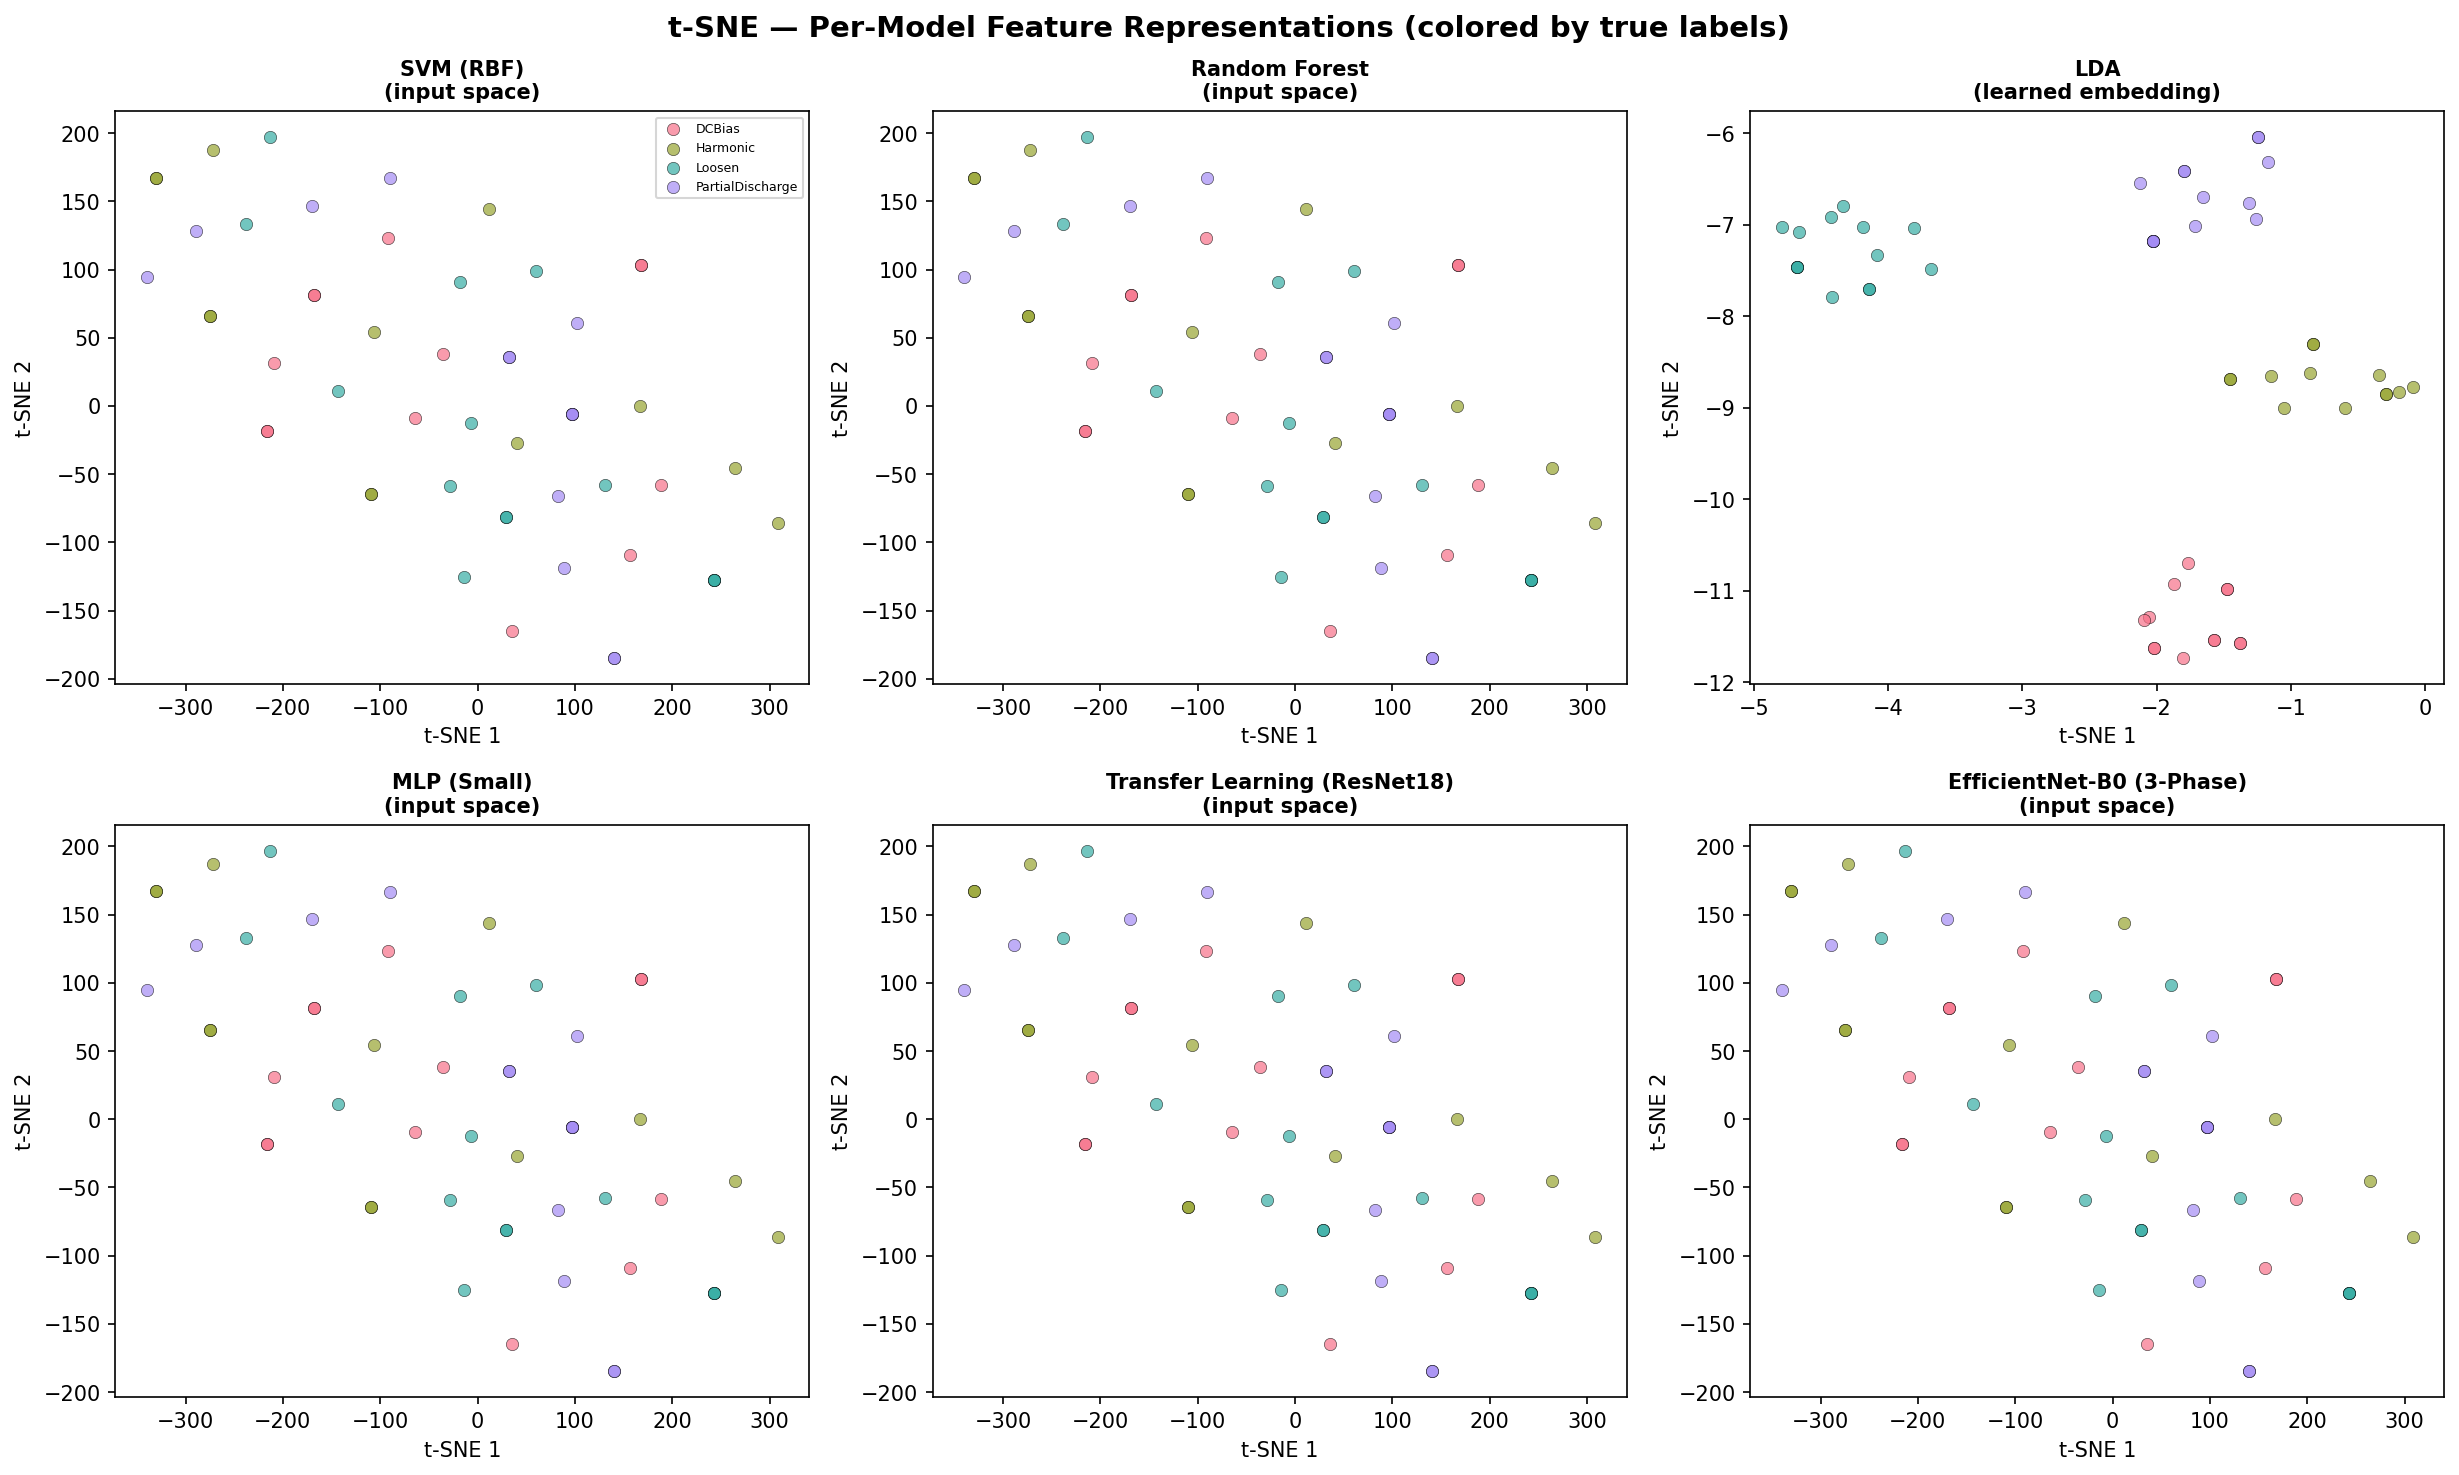
\includegraphics[width=1\linewidth]{results/tsne_per_model}
\caption{}
\label{}
\end{figure*}




% The signal comparison figure before and after mvdr are shown in Fig. \ref{Signal_comparison_input_vs_mvdr}. 

% \begin{figure*}
% \centering
% 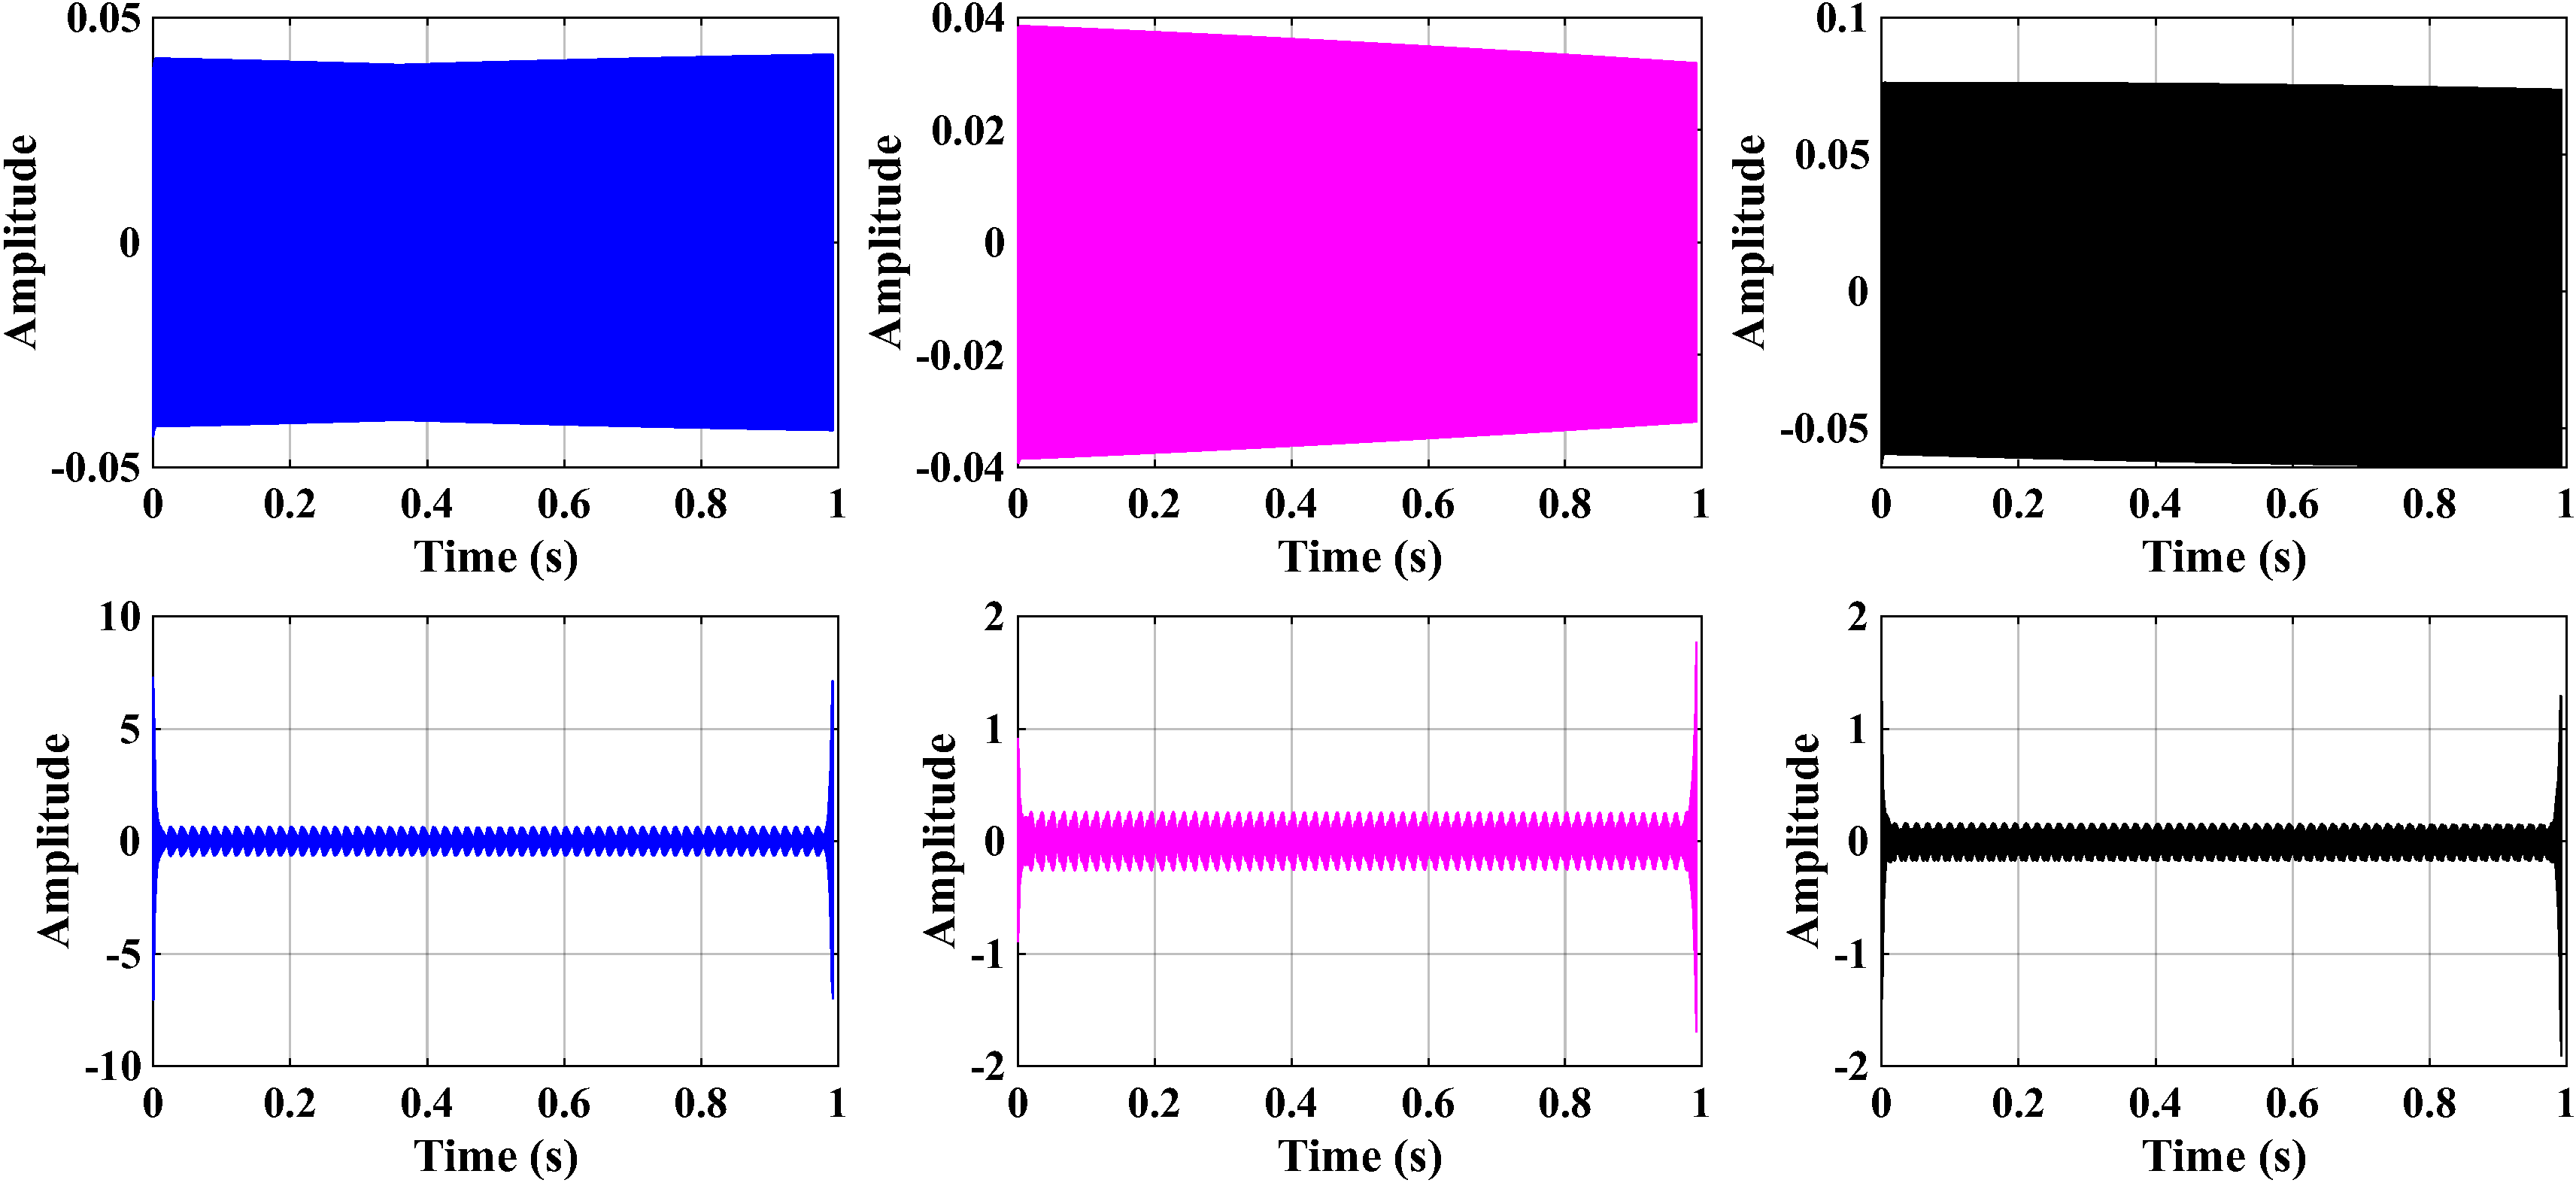
\includegraphics[width=1\linewidth]{output/demo_2k_4k/figures/Signal_comparison_input_vs_mvdr}
% \caption{Spectrogram comparison between the input signal (left) and the MVDR beamformed output signal (right). The MVDR output shows significant suppression of interference components while preserving the target signal.}
% \label{Signal_comparison_input_vs_mvdr}    
% \end{figure*}


% The SNR improvement is calculated to quantify the enhancement of the target signal relative to the interference and noise. The input SNR is computed based on the power of the target signal and the combined power of interference and noise in the original multichannel signals. The output SNR is calculated similarly for the MVDR beamformed output signal. As shown in Fig. \ref{fig:snr_improvement}, the difference between the output SNR and input SNR provides a measure of the improvement achieved by the MVDR beamforming process.

% \begin{equation}
% SNR = 10 \cdot \log_{10} \left( \frac{P_{\text{target}}}{P_{\text{interference}} + P_{\text{noise}}} \right)
% \end{equation}

% \begin{equation}
%     \Delta \text{SNR} = \text{SNR}_{out} - \text{SNR}_{in}
% \end{equation}



% \begin{figure}
% \centering
% 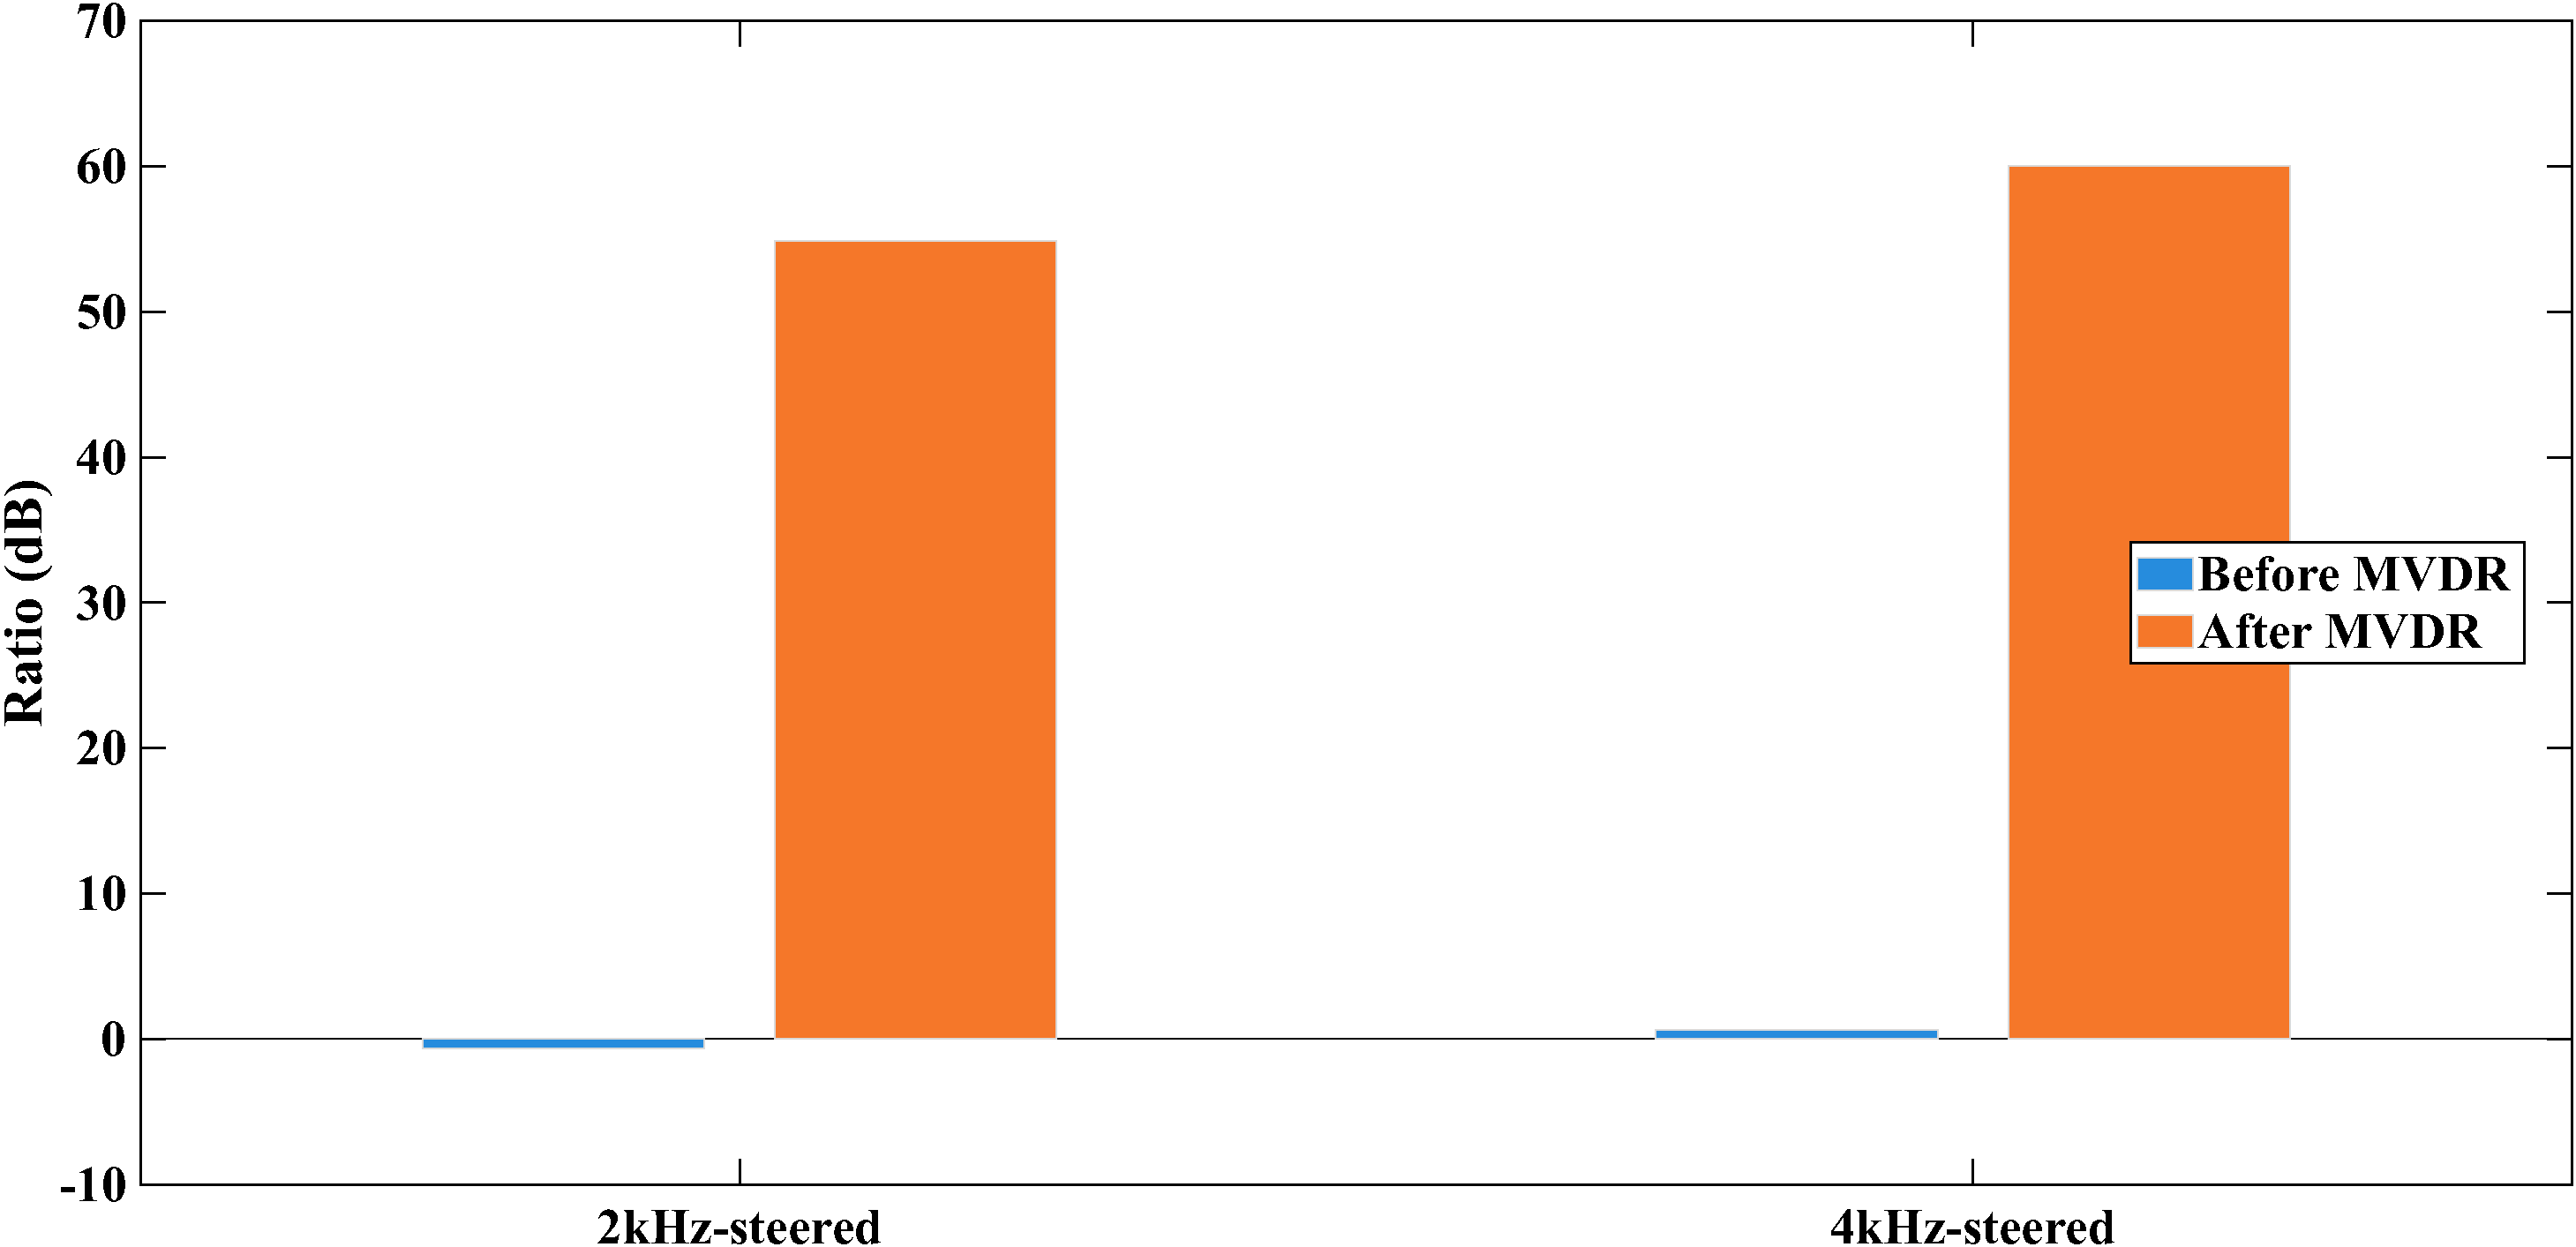
\includegraphics[width=1\linewidth]{output/real_signal/figures/Performance_improvement}
% \caption{SNR improvement of the MVDR beamforming process. The output SNR is significantly higher than the input SNR, indicating effective enhancement of the target signal relative to interference and noise
% .}
% \label{fig:snr_improvement}
% \end{figure}

% The Signal-to-Interference-plus-Noise Ratio (SINR) improvement is calculated to assess the effectiveness of the MVDR beamforming in enhancing the target signal under strong interference conditions.

% \begin{equation}
% SINR = 10 \cdot \log_{10} \left( \frac{P_{\text{interference}}}{P_{\text{target}} + P_{\text{noise}}} \right)
% \end{equation}


% \subsection{Hardware Platform and Experimental Measurements}

% \subsubsection{Data Acquisition System}

% The experimental system comprises:
% \begin{enumerate}
%     \item \textbf{128-Channel Multi-Arm Spiral Microphone Array}: Captures acoustic signals from equipment
%     \item \textbf{MEMS Acquisition Board}: Converts analog acoustic signals to PDM (Pulse Density Modulation) digital format
%     \item \textbf{UDP Communication Link}: Transmits captured data to PC for real-time MVDR processing
%     \item \textbf{PC-Based Processing}: Executes MVDR algorithms and generates diagnostic features
% \end{enumerate}

% \subsubsection{Experimental Setup}

% Experiments are conducted in a $12m \times 12m \times 4m$ laboratory:
% - \textbf{Array Position}: 1 m above floor, vertical orientation perpendicular to floor
% - \textbf{Sound Sources}: Two loudspeakers arranged adjacently and parallel
%   - Speaker 1: Transformer fault signal (target)
%   - Speaker 2: Interference signal
% - \textbf{Source Spacing}: 50 cm horizontal separation
% - \textbf{Source Height}: 1 m above floor, same plane parallel to array plane

% \subsubsection{MVDR Processing Details}

% Key implementation aspects:
% \begin{enumerate}
%     \item \textbf{Window Selection}: Hamming window with 50\% frame overlap to minimize spectral leakage
%     \item \textbf{Numerical Stability}: Diagonal loading (Tikhonov regularization) applied when covariance matrix condition number exceeds predefined threshold
%     \item \textbf{Frequency Band}: Limited to relevant frequencies [300 Hz, 8000 Hz] for fault diagnosis
%     \item \textbf{Covariance Averaging}: Moving average over 31 consecutive frames for robust estimation
%     \item \textbf{Regularization Parameter}: $\epsilon = 10^{-4}$ for numerical stability
% \end{enumerate}




% \subsection{Network Architecture and Training Strategy}

% \subsubsection{Convolutional Neural Network for Feature Extraction}

% A convolutional neural network (CNN) is employed for automatic feature extraction from spectrograms:
% \begin{itemize}
%     \item \textbf{Input}: Time-frequency spectrograms from MVDR-processed signals
%     \item \textbf{Architecture}: 
%         - Multiple convolutional layers with ReLU activation
%         - Max-pooling layers for dimension reduction
%         - Batch normalization for stable training
%         - Dropout layers for regularization
%     \item \textbf{Feature Maps}: Progressive increase in feature dimensionality
%     \item \textbf{Output}: Flattened feature vector for classification
% \end{itemize}

% \subsubsection{Fully Connected Classification Layers}

% Extracted features are processed through fully connected layers:
% \begin{itemize}
%     \item \textbf{Hidden Layers}: Multiple dense layers with dropout regularization
%     \item \textbf{Activation}: ReLU for hidden layers, softmax for output layer
%     \item \textbf{Output Neurons}: Corresponds to number of fault classes
% \end{itemize}

% \subsubsection{Training Procedure}

% Training parameters and strategy:
% \begin{itemize}
%     \item \textbf{Loss Function}: Cross-entropy loss
%     \item \textbf{Optimizer}: Adam with adaptive learning rate
%     \item \textbf{Batch Size}: Configurable (typically 32 or 64)
%     \item \textbf{Epochs}: Training until convergence with early stopping
%     \item \textbf{Validation}: 20\% of training data reserved for validation
%     \item \textbf{Data Augmentation}: Spectral masking and time shifting for robustness
% \end{itemize}

% \subsection{Fault Classes and Data Preparation}

% The training dataset includes spectrograms from different fault conditions:
% \begin{enumerate}
%     \item Normal operation (baseline)
%     \item Bearing wear/degradation
%     \item Winding faults
%     \item Mechanical imbalance
%     \item [Additional fault types as applicable]
% \end{enumerate}

% Each class consists of multiple recordings under varying environmental conditions and noise levels.

% \subsection{Performance Metrics and Evaluation}

% \subsubsection{Classification Metrics}

% Model performance is evaluated using:
% \begin{itemize}
%     \item \textbf{Accuracy}: Overall correct classification rate
%     \item \textbf{Precision}: Fraction of positive predictions that are true positives
%     \item \textbf{Recall}: Fraction of actual positives correctly identified
%     \item \textbf{F1-Score}: Harmonic mean of precision and recall
%     \item \textbf{Confusion Matrix}: Detailed breakdown of classification results
% \end{itemize}

% \subsubsection{Robustness Analysis}

% Robustness under adverse conditions:
% \begin{itemize}
%     \item Performance under varying SNR levels
%     \item Generalization to unseen environmental conditions
%     \item Stability against sensor variations or microphone degradation
% \end{itemize}

\section{Conclusions}
\label{conclusion}
This paper presents a comprehensive framework for electrical equipment fault diagnosis based on microphone array beamforming and deep learning. The key contributions are:

\begin{enumerate}
    \item \textbf{STFT-FD Beamforming}: A frequency-dependent STFT approach providing adaptive time-frequency resolution, enabling optimal analysis of wideband fault signals
    
    \item \textbf{Wideband MVDR Implementation}: Frequency-domain MVDR processing on a 128-element multi-arm spiral array achieves significant interference suppression (22.66 dB SINR improvement) without manual delay compensation
    
    \item \textbf{RIR-Based Signal Modeling}: Acoustic environment modeling via room impulse responses provides realistic simulation without manual inter-channel delay specification
    
    \item \textbf{Integrated Diagnosis System}: Combining array signal processing with deep learning enables robust fault classification under strong interference and noise
    
    \item \textbf{Practical Implementation}: Hardware platform utilizing MEMS microphone arrays and real-time UDP communication demonstrates feasibility for field deployment
\end{enumerate}

The experimental results demonstrate that the proposed system significantly outperforms single-channel approaches in both signal enhancement and fault classification performance. The combination of spatial filtering via MVDR beamforming and feature learning via deep neural networks provides a robust, practical solution for acoustic fault diagnosis in industrial environments.

Future work includes:
\begin{itemize}
    \item Extended evaluation on diverse equipment types and fault conditions
    \item Optimization of computational complexity for embedded system deployment
    \item Development of transfer learning approaches for rapid adaptation to new equipment
    \item Integration with predictive maintenance scheduling systems
\end{itemize}

\appendix

\section{Lagrange Multiplier Method for Optimal Weight Vector Derivation}

The constrained MVDR optimization problem can be solved using the method of Lagrange multipliers, converting the constrained problem to an unconstrained one through:

\begin{equation}
\mathcal{L}(\boldsymbol{w}(k), \lambda) = \boldsymbol{w}^H(k) \boldsymbol{R}_{xx}(k) \boldsymbol{w}(k) - \lambda \left[ \boldsymbol{w}^H(k)\boldsymbol{a}(k, \theta_0, \phi_0) - 1 \right]
\end{equation}

where $\lambda$ is the Lagrange multiplier.

Taking the derivative with respect to $\boldsymbol{w}^H(k)$ and setting it to zero:

\begin{equation}
\frac{\partial \mathcal{L}}{\partial \boldsymbol{w}^H(k)} = \boldsymbol{R}_{xx}(k) \boldsymbol{w}(k) - \lambda \boldsymbol{a}(k, \theta_0, \phi_0) = 0
\end{equation}

Rearranging yields the weight vector expression:

\begin{equation}
\boldsymbol{w}(k) = \lambda \boldsymbol{R}_{xx}^{-1}(k)\boldsymbol{a}(k, \theta_0, \phi_0)
\end{equation}

Substituting into the distortionless constraint $\boldsymbol{w}^H(k)\boldsymbol{a}(k, \theta_0, \phi_0) = 1$:

\begin{equation}
\lambda \boldsymbol{a}^H(k, \theta_0, \phi_0) \boldsymbol{R}_{xx}^{-1}(k)\boldsymbol{a}(k, \theta_0, \phi_0) = 1
\end{equation}

Solving for the Lagrange multiplier:

\begin{equation}
\lambda = \frac{1}{\boldsymbol{a}^H(k, \theta_0, \phi_0) \boldsymbol{R}_{xx}^{-1}(k)\boldsymbol{a}(k, \theta_0, \phi_0)}
\end{equation}

Substituting $\lambda$ back into the weight vector expression yields the MVDR optimal weight at frequency bin $k$:

\begin{equation}
\boldsymbol{w}_{\text{MVDR}}(k) = \frac{\boldsymbol{R}_{xx}^{-1}(k)\boldsymbol{a}(k, \theta_0, \phi_0)}{\boldsymbol{a}^H(k, \theta_0, \phi_0)\boldsymbol{R}_{xx}^{-1}(k)\boldsymbol{a}(k, \theta_0, \phi_0)}
\end{equation}

When the covariance matrix is rank-deficient, the regularized form $\boldsymbol{R}_{xx}^{\text{DL}}(k) = \boldsymbol{R}_{xx}(k) + \epsilon \mathbf{I}$ (Tikhonov regularization with diagonal loading parameter $\epsilon$) is employed to ensure numerical stability.

\bibliographystyle{IEEEtran}
\bibliography{MVDR}

\end{document}
